\chapter{Talen en Automaten}\label{chap:talenautomaten}

\section{Inleiding}


Informatici hebben veel te maken met programma's, en programma's
berekenen dikwijls bij een gegeven input een output. Dat moet heel
ruim opgevat worden: input kan een elektrisch signaal zijn dat een
temperatuursschommeling aanduidt, een karakter dat van het toetsenbord
komt, een programma, een gegevensbank ... en de bijbehorende output
kan dan een rij signalen zijn om klepopeningen te regelen, een
aangepast document, een bestand met foutenboodschappen, een display
met gevraagde gegevens ...


Vanuit praktisch standpunt zijn bovenstaande voorbeelden heel
verschillend en als we te veel naar de details van de voorbeelden
kijken, dan missen we veel, want er is een kader dat abstractie van
vele details maakt en waarin elk van die voorbeelden te beschrijven
valt: het gaat steeds om een mapping van elementen die uit een
inputdomein komen, naar een element uit een outputdomein. Die domeinen
zijn altijd discreet, maar soms wel onbegrensd groot.  Vanuit
theoretisch standpunt zijn programma's dus altijd terug te brengen tot
functies van (een deel van) $\N$ naar (een deel van) $\N$.  


Als het inputdomein klein is, dan is de functie niet erg interessant:
je kan een tabel aanleggen en de functiewaarde voor een gegeven input
berekenen is een simpele lookup.\footnote{Tabulatie is in deze context
een interessante dynamische implementatietechniek, zowel in
functioneel (inclusief OO) als in logisch programmeren (waar relaties
worden gespecifieerd i.p.v. functies). Wil je meer weten, vraag !}


Als het inputdomein groot is, of niet a priori bekend, dan is het
voordien tabuleren van de functie niet mogelijk, en is het beter van
te doen alsof het inputdomein oneindig groot is.  

Het outputdomein moet minstens twee elementen bevatten om een
interessante functie te verkrijgen. Die twee elementen zouden {\em ja,
nee} kunnen zijn en laten toe om {\em beslissingsproblemen} te
beschrijven: problemen waarbij je wil weten of een input voldoet aan
een bepaalde eigenschap, zoals {\em is dit programma syntactisch
correct?}, of nog {\em is vandaag een goede dag om te beleggen in
FCW?} \footnote{Ja !}  ...  

Als het outputdomein meer dan twee, maar wel eindig veel elementen
bevat, dan is het gemakkelijk om door een rij ja-nee vragen over de
input, de juiste output te verkrijgen. Stel dat je wil berekenen op
welke dag van de week je best in FCW belegt, dan stel je de volgende
ja-nee vragen: {\em is maandag de beste dag om in FCW te beleggen
?}, {\em is dinsdag de beste dag om in FCW te beleggen?}, 
{\em is woensdag de beste dag om in FCW te beleggen?}, ...
Van de eindige outputdomeinen, zijn dus alleen die met juist twee
waarden echt interessant.


Als het outputdomein oneindig groot is, dan kunnen we dat niet zomaar
reduceren naar een eindige rij functies met eindig outputdomein.


We besluiten dat er maar twee soorten interessante functies bestaan:
functies met signatuur $\N \rightarrow\{ja,nee\}$ en functies met
signatuur $\N \rightarrow \N$. 

Laat ons nog eens naar die eerste klasse kijken: er is een zekere
structuur en semantiek geassocieerd met het outputdomein, maar het
inputdomein is zeer generisch. $\N$ staat immers voor een willekeurige
aftelbare oneindige verzameling: een andere aftelbare oneindige
verzameling zou net zo goed kunnen dienen. Verder: als we elementen
van $\N$ noteren, dan gebruiken we (bijvoorbeeld) de tien decimale
cijfers en vormen daarmee strings (rijen van decimale cijfers), maar
we hadden net zo goed in een andere basis kunnen werken, bijvoorbeeld
binair, of hexadecimaal, of op nog totaal andere manier de elementen
van $\N$ voorstellen: excess-3, ...  Die voorstellingswijzen hebben
gemeen dat ze gebruik maken van een eindig aantal symbolen, dat de
voorstelling uniek is en dat als je twee voorstellingen (van twee
gelijke of verschillende) getallen achter elkaar plaatst, je de
voorstelling krijgt van een nieuw getal.  De eindige verzameling van
symbolen noemen we een alfabet, en gelijk welke eindige rij symbolen
stelt een getal voor. Stel met $\Sigma$ een eindig alfabet voor, en
met $\Sigma^*$ alle eindige rijen van symbolen uit $\Sigma$. Dan
hebben we nu juist zowat verantwoord dat we functies zullen bekijken
met signatuur $\Sigma^* \rightarrow \{ja,nee\}$. Een functie $F$ van
die klasse wordt nu helemaal bepaald door de verzameling symboolrijen
$s$ waarvoor geldt dat $F(s) = ja$ en we kunnen i.p.v. zulke functies
te bekijken, net zo goed naar deelverzameling $V$ van $\Sigma^*$
kijken met de bijbehorende vraag {\em behoort een gegeven s tot
$V$}. Het is belangrijk om te beseffen dat we geen echt grotere
klasse van functies beschouwen dan $\N \rightarrow\{ja,nee\}$, maar
ook dat het dikwijls beter is om beslissingsproblemen op meer
natuurlijke manier te beschrijven, t.t.z. vanuit het standpunt van
delen van $\Sigma^*$. Bijna alle theorie i.v.m. berekenbaarheid zal
geformuleerd worden in dit kader.  

De tweede klasse functies met signatuur ($\N \rightarrow \N$) zullen
iets minder aan bod komen, maar ze zijn natuurlijk heel belangrijk.

\newpage
\paragraph{Zelf doen:}
\begin{itemize}
\item[]

De inleiding maakt vereenvoudigingen of veronderstellingen waarmee je
misschien niet akkoord gaat, of die op zijn minst argumentatie
vereisen. Zoek mogelijke {\em gaten} in de inleiding, bedenk
alternatieven, argumenteer voor en tegen ...

Beschrijf een beslissingsprobleem dat je al kende met behulp van
een alfabet en een deelverzameling die de oplossing van het probleem
is. Doe dat voor een probleem met cijfers en getallen, een probleem
met letters en woorden, ... Zorg dat je telkens een probleem kiest
waarvoor de deelverzameling eindig is, en eentje waarvoor de
deelverzameling oneindig is. Wat als je ja/nee omkeert?

\end{itemize}

\section{Wat is een taal?}


De inleiding motiveert om beslissingsproblemen te bekijken. Een
beslissingsprobleem komt overeen met een deelverzameling van de rijen (ook
strings genoemd) die je kan maken met elementen uit een alfabet
$\Sigma$.  Zulk een deelverzameling noemen we een {\em taal} over
$\Sigma$. Elementen uit de taal noemen we {\em woorden} of {\em
strings}. Een alfabet heeft altijd een eindig aantal elementen.

\grijs{\begin{definitie} String over een alfabet $\Sigma$\\
{\rm
Een {\bf string} over een alfabet $\Sigma$ is een opeenvolging van
nul, \'{e}\'{e}n of meer elementen van $\Sigma$
}
\end{definitie}}

Het is duidelijk dat als we twee strings $x$ en $y$ achter elkaar
zetten, we een nieuwe string krijgen. We noteren die met $xy$.


\grijs{\begin{definitie} Taal L over een alfabet $\Sigma$\\
{\rm
Een {\bf taal} $L$ over een alfabet $\Sigma$ is een verzameling van
eindige strings over $\Sigma$
}
\end{definitie}}

Een taal kan eindig zijn of oneindig. Als een taal L oneindig is, is L
dan aftelbaar?\footnote{als je niet meer weet wat aftelbaar is, zoek
het op}

Om een taal vast te leggen moet je een beschrijving geven van elk
element van de taal. Bijvoorbeeld: de taal van even getallen (over een
alfabet van decimale cijfers) bevat juist alle getallen die eindigen
op een 0, 2, 4, 6 of 8. Een ander voorbeeld: elk woord dat rijmt op
fantastisch. Of nog: elke ...

Een beschrijving van elk element van een taal is liefst eindig, zelfs
als de taal oneindig is.


Een beschrijving van elk element van een taal kan je (meestal)
gebruiken om na te gaan of een string tot de taal behoort, maar
(meestal) ook om elk element van de taal te construeren of genereren.
Let hier goed op de {\em (meestal)}: daarover komen later vragen.

Als de beschrijving van een taal eenvoudig is, dan verwachten we dat
de taal eenvoudig is - maar hebben we wel een goed beeld van wat
eenvoudig is? 

Hier zijn nog wat vragen om je over te bezinnen en waarop in deze
cursus antwoorden worden aangereikt:

\begin{itemize}
\item 
Bestaat er een formalisme om taalbeschrijvingen te noteren?

\item 
Geeft dat formalisme aanleiding tot het (automatisch) afleiden van
testers en generators van de taal?

\item 
Bestaan er talen die niet in een formalisme kunnen gevat worden?

\item
Wat is de goede notie van testen? En genereren?

\item
Zijn sommige talen inherent gemakkelijker dan andere om te

beschrijven/testen/genereren?

\end{itemize}

Tenslotte is er de vraag:

\begin{itemize}
\item[] Waarom moet een universitaire informaticus dit kennen?
\end{itemize}


\paragraph{Zelf doen:}
\begin{itemize}
\item[]

Kan je een beschrijving van de even getallen gebruiken om alle even
getallen te genereren?

Alle woorden rijmend op fantastisch?

Hoe zit het met testen?

Verzin zelf een taal, een beschrijving van die taal en gebruik die
beschrijving om te testen of een gegeven string tot de taal behoort,
en ook om alle strings van de taal te genereren. Hoe extravaganter de
taal is, hoe beter.

Zie je in je voorbeelden een verband tussen hoe eenvoudig het is om je
taal te beschrijven en testen of te genereren?

Heb je al een gevoel voor de andere vragen die hiervoor gesteld werden?
\end{itemize}

\newpage
\section{Een algebra van talen}

Een algebra - of algebraische structuur - is een verzameling met
daarop een aantal inwendige operaties: dikwijls binaire operaties,
maar unair of met grotere ariteit kan ook. Zo wordt de verzameling van
alle talen over een alfabet $\Sigma$ een algebra als we als operaties
unie, doorsnede, complement ... defini\"eren. Meer concreet:
%
als $L_1$ en $L_2$ twee talen zijn, dan is

\begin{itemize}
\item de unie ervan een taal: $L_1 \cup L_2$
\item de doorsnede ervan een taal: $L_1 \cap L_2$
\item het complement ervan een taal: $\overline{L_1}$
\end{itemize}

Daarmee kan je nog andere operaties maken.

Een nieuwe manier om uit twee talen een taal te maken is {\em
concatenatie}:

\grijs{\begin{definitie} Concatenatie van twee talen\\
{\rm
Gegeven twee talen $L_1$ en $L_2$ over hetzelfde alfabet $\Sigma$, dan
noteren we de concatenatie van $L_1$ en $L_2$ als $L_1L_2$ en
defini\"eren we: \\
$L_1L_2 = \{xy | x \in L_1, y \in L_2\}$
}
\end{definitie}}

We hebben geen haakjes gezet rond de concatenatie van talen, want het
is duidelijk dat concatenatie associatief is, t.t.z.
%
$(L_1L_2)L_3 = L_1(L_2L_3)$


Als we $L$ n keer concateneren met zichzelf, noteren we dat door $L^n$.
$L^0$ bevat alleen de lege string die we noteren door $\epsilon$.

Tenslotte defini\"eren we nog een operatie die toelaat om oneindige
talen te construeren vanuit een eindige taal:

\grijs{\begin{definitie} $L^*$ - de Kleene {\bf ster} van een taal $L$\\
{\rm

$~~~~~~~~~~~~~~~~~~~~~~~L^* = \cup_{n=0}^\infty L^n$
}
\end{definitie}}

Als afkorting voor $LL^*$ wordt $L^+$ gebruikt.

Met die notatie kunnen we nu een taal $L$ defini\"eren als een
deelverzameling van $\Sigma^*$, of equivalent daarmee
%
$ L \in {\cal P}(\Sigma^*)$

\paragraph{Zelf doen:} zoek nieuwe operaties die van een taal een (mogelijke nieuwe) taal maken.

\newpage

\section{Talen beschrijven}


In de wiskunde gebruikt men verzamelingennotatie om verzamelingen te
beschrijven. Bijvoorbeeld:

\begin{vb}
Met $\Sigma = \{x,y,z\}$:
\begin{itemize}
\item 
$\Sigma^* = \{a_1a_2a_3...a_n|a_i \in \Sigma, n \in \N \}$
\item 
$L = \{a_1a_2a_3...a_n|a_1 = y, n \in \N, \forall i > 1: a_i \in \Sigma\}$

L is de verzameling van strings die met y beginnen.
\end{itemize}
\end{vb}




Ook informele beschrijvingen kunnen, zolang ze maar ondubbelzinnig
zijn zodat elk {\em ding} een element is of niet:

\begin{vb}
~~
\begin{itemize}
\item 
$H(n) = \{P | P~is~een~Javaprogramma~en~P~stopt~na~hoogstens~n~seconden~bij~input~n\}$
\item 
$Prime = \{n|n \in \N, n~is~een~priemgetal\}$
\end{itemize}
\end{vb}

Die laatste is ook informeel, maar er zit natuurlijk een definitie van
priemgetal achter die formeel kan uitgeschreven worden. Zoiets als 

\hspace{1cm}$Prime = \{n|n \in \N, \forall i:1<i<n \rightarrow n~mod~i \neq 0\}$

Voor ons is zulke beschrijving echter niet genoeg: wij willen een
formalisme dat beter toelaat om strings te genereren en te testen.
Dat bestaat al voor natuurlijke talen: een grammatica voor het
nederlands beschrijft de structuur van een nederlandse zin.
Nederlands is echter een ingewikkelde taal, met een complexe structuur
en veel uitzonderingen: het heeft zin om eerst een klasse meer eenvoudige
talen te bestuderen.


We werken toe naar een 
\begin{itemize}
\item[]
hi\"erarchie van talen

\item[]
met bijbehorende hi\"erarchie van beschrijvingsmechanismen of grammatica's

\item[]
met bijbehorende hi\"erarchie van {\em test} en  {\em generatie} procedures

\end{itemize}

Die hi\"erarchie heet de {\em Chomsky-hi\"erarchie\footnote{Noam
Chomsky}}. We beginnen onderaan, t.t.z. bij de {\em gemakkelijke} talen
...


\newpage

\section{Reguliere expressies en reguliere talen}

\grijs{\begin{definitie} \label{defregexp} Reguliere Expressie
(RE) over een alfabet $\Sigma$\\
{\rm E is een {\bf reguliere expressie over alfabet $\Sigma$} indien E
van de vorm is
\begin{itemize}
\item $\epsilon$
\item $\phi$
\item $a$ waarbij $a \in \Sigma$
\item $(E_1E_2)$ waarbij $E_1$ en $E_2$ reguliere expressies zijn over $\Sigma$
\item $(E_1)^*$ waarbij $E_1$ een reguliere expressie is over $\Sigma$
\item $(E_1 | E_2)$ waarbij $E_1$ en $E_2$ reguliere expressies zijn over $\Sigma$
\end{itemize}
}
\end{definitie}}

Hierboven is de verzameling van reguliere expressies {\em RegExps}
op inductieve manier gedefinieerd. Er is onder verstaan dat iets dat
niet onder de definitie valt, geen reguliere expressie is. Dikwijls is
het impliciet duidelijk welk alfabet we gebruiken en vermelden we het
niet meer. We gebruiken haakjes zodat er geen enkele ambigu\"{i}teit kan
bestaan: haakjes behoren niet tot het alfabet. In de volgende
voorbeelden is $\Sigma = \{a,b,c\}$.


\begin{vb}
Reguliere expressies over $\Sigma$:
\begin{itemize}
\item b
\item a($\epsilon$c)
\item $(((ab))^*c~|~(bc))$
\end{itemize}
\end{vb}

Gebruiken we te veel haakjes - of te weinig? Waarom?



\grijs{\begin{definitie} Een reguliere expressie E {\bf bepaalt} een taal $L_E$ over
hetzelfde alfabet $\Sigma$ als volgt:
\newpage
{\rm
\begin{itemize}
\item als E = a (met $a \in \Sigma$) dan is $L_E = \{a\}$ (de taal met
\'{e}\'{e}n string die enkel het teken a is)
\item als E = $\epsilon$ dan is $L_E = \{\epsilon\}$ (de lege string)
\item als E = $\phi$ dan is $L_E = \emptyset$ (de lege verzameling)
\item als E = $(E_1E_2)$ dan $L_E = L_{E_1}L_{E_2}$
\item als E = $(E_1)^*$ dan $L_E = L_{E_1}^*$
\item als E = $(E_1 | E_2)$ dan $L_E = L_{E_1} \cup L_{E_2}$
\end{itemize}
}
\end{definitie}}

Die overeenkomst tussen een reguliere expressie en een taal maakt dat
we in reguliere expressies ook wegkomen met minder haakjes:
concatenatie van talen is immers associatief en als we afspreken dat
de $^*$ sterker bindt dan concatenatie die sterker bindt dan unie, dan
kunnen veel haakjes weg.

\paragraph{Zelf doen:}
Geef een woordelijke beschrijving van de talen die bepaald worden door
de volgende RE's over $\{a,b\}$ - de eerste dient als voorbeeld:

\begin{itemize}
\item[]
$(ab)^*$: elke a wordt direct door een b gevolgd en er zijn evenveel a's als
b's

$(aba)^*$

$(a|b)^*$

$(a|b)^*\phi$

$a \epsilon b$
\end{itemize}


\paragraph{Zelf doen:}
Bewijs de volgende uitspraken, of geef een tegenvoorbeeld:

\begin{itemize}
\item[]
als een reguliere expressie E geen $^*$ bevat, dan is $L_E$ eindig

als een reguliere expressie E $^*$ bevat, dan is $L_E$ oneindig

$L_E \subseteq L_{(E|F)}$ voor alle RE's E en F

de verzameling van alle reguliere expressies (over een gegeven
alfabet) is zelf een taal (en over welk alfabet?)

de verzameling van alle reguliere expressies (over een gegeven
alfabet) is zelf een reguliere taal
\end{itemize}


\medskip


\grijs{\begin{definitie}Reguliere Taal \\
{\rm
Een taal die door een reguliere expressie bepaald wordt is een {\bf reguliere taal}.
}
\end{definitie}}



Is het duidelijk dat een reguliere taal een taal is? De verzameling van
reguliere talen duiden we aan met $RegLan$. Kijk na welke van volgende
formules zin hebben, en welke juist zijn.

\begin{enumerate}
\item $RegLan \subseteq \Sigma$
\item $RegLan \subseteq \Sigma^*$
\item $RegLan \subseteq {\cal P}(\Sigma)$
\item $RegLan \subseteq {\cal P}(\Sigma^*)$
\item $RegLan \subseteq {\cal P}({\cal P}(\Sigma^*))$
\item indien $x \in RegLan$ dan $x \in \Sigma$
\item indien $x \in RegLan$ dan $x \in \Sigma^*$
\item indien $x \in RegLan$ dan $x \in {\cal P}(\Sigma)$
\item indien $x \in RegLan$ dan $x \in {\cal P}(\Sigma^*)$
\item indien $x \in RegLan$ en $y \in x$ dan $y \in \Sigma$
\item indien $x \in RegLan$ en $y \in x$ dan $y \in \Sigma^*$
\item indien $x \in RegLan$ en $y \in x$ dan $y \in {\cal P}(\Sigma)$
\item indien $x \in RegLan$ en $y \in x$ dan $y \in {\cal P}(\Sigma^*)$
\end{enumerate}

\paragraph{Zelf doen:}

\begin{itemize}
\item[]
Is de volgende uitspraak juist? {\em voor elke reguliere taal L
bestaat een reguliere expressie E zodanig dat $L_E = L$}.


Is het duidelijk dat er talen zijn die NIET regulier zijn?

Is elke eindige taal regulier?

Is elke oneindige reguliere taal aftelbaar?

Is het mogelijk om gegeven een reguliere taal de bijhorende reguliere
expressie te construeren?

Als je een string s krijgt en een reguliere expressie E, kan je dan
(gemakkelijk) bepalen of $s \in L_E$?

Kan je alle strings in $L_E$ genereren als je E krijgt?
\end{itemize}


\section{De subalgebra van reguliere talen}

De verzameling van talen over een alfabet $\Sigma$ noteren we met
$L_\Sigma$. Ze vormt een algebra: de verzameling zelf is ${\cal
P}(\Sigma^*)$ = $L_\Sigma$.


Als we twee talen $L_1$ en $L_2$ uit $L_\Sigma$ nemen, dan kunnen we
die gebruiken om de taal $L_1L_2$ te maken (concatenatie van talen),
de taal $L_1 \cup L_2$ (unie van talen), de taal $L_1^*$
(willekeurig lange concatenatie) en de complementstaal $\overline{L_1}$. Het
resultaat zit terug in $L_\Sigma$. Dus: $L_\Sigma$ is een algebra met
(minstens) vier inwendige operaties.


Vermits $RegLan \subseteq L_\Sigma$ is het zinvol om te vragen of
RegLan een subalgebra is van $L_\Sigma$: daarvoor moeten de operaties
ook inwendig zijn op RegLan.


Formuleer de stelling die uitdrukt dat RegLan een subalgebra is van
$L_\Sigma$ en bewijs je stelling op een constructieve manier,
t.t.z. construeer o.a. een E zodanig dat $L_E = L_{E_1} \cup L_{E_2}$.
Heb je een probleem met het complement van een reguliere taal?


\clearpage

\section{Eindige toestandsautomaten}

Eindige toestandsautomaten zijn bedoeld om talen mee te beschrijven -
testen en genereren van strings horen daarbij. Eindige
toestandsautomaten kunnen grafisch voorgesteld worden en daarmee
beginnen we: later geven we een formele definitie. Figuur~\ref{fsa1}
toont een eerste voorbeeld van een NFA\footnote{Onze afkorting voor
een eindige toestandsautomaat: we verklaren die later wel.} over het
alfabet $\{a,b,c\}$.

\begin{figure}[h]
\begin{center}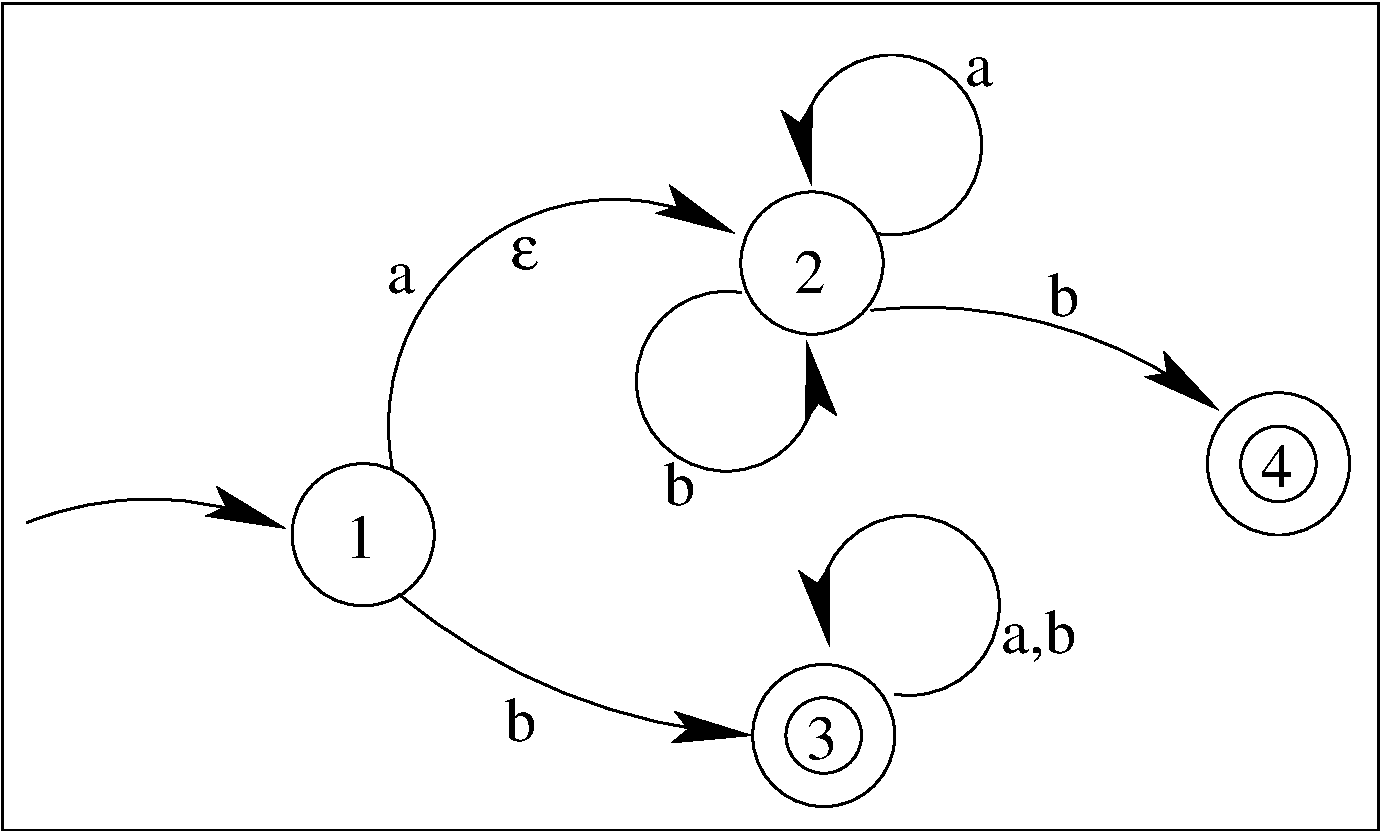
\includegraphics[%
  width=0.5\linewidth,
  keepaspectratio]{fsa1}\end{center}
\caption{Een eindige toestandsautomaat\label{fsa1}}
\end{figure}

De belangrijke kenmerken:

\begin{itemize}
\item we zien een gerichte graaf
\item de knopen hebben een naam (hier een getal) - de knopen noemen we toestanden
\item er zijn twee soorten knopen: knopen met een dubbel cirkeltje
getekend noemen we (aanvaardende) eindtoestanden
\item lussen zijn toegestaan (bogen van een knoop naar dezelfde knoop)
\item de bogen dragen een label (soms meer dan \'{e}\'{e}n); dat label
is een symbool uit het alfabet, of meerdere symbolen uit het alfabet
(gescheiden door een komma) en/of $\epsilon$
\item er is slechts \'{e}\'{e}n boog die niet vertrekt in een knoop;
die boog komt aan in een knoop die we de starttoestand noemen
\end{itemize}

We gebruiken de grafische voorstelling van de NFA als volgt:

\begin{enumerate}
\item je krijgt een string $s$ over het alfabet in handen en vertrekt
ermee in de starttoestand
\item je mag nu van \'{e}\'{e}n toestand naar een andere gaan door
een boog te volgen en in je vertrektoestand een symbool achter te
laten dat op de boog staat en van voor in je string staat: je string
wordt daardoor korter; als de boog ook $\epsilon$ bevat, dan hoef je
niet een teken achter te laten
\item blijf overgangen maken: als je aankomt in een eindtoestand en
je string is leeg op dat ogenblik, dan zeggen we {\em de NFA heeft de
initi\"ele string $s$ aanvaard}
\end{enumerate}

Dit geeft ons slechts een informele definitie van aanvaarde string!


Hier is een tweede manier om die grafische voorstelling te gebruiken:

\begin{enumerate}
\item vertrek met een lege string in de starttoestand
\item volg nu willekeurig bogen van de toestand waarin je bent, naar
een volgende toestand: als op die boog een symbool staat, voeg het
vanachter toe aan je huidige string; blijf rondlopen
\item telkens je in een eindtoestand arriveert, en je hebt string s
opgebouwd ondertussen, roep luid {\em deze machine aanvaardt s}
\end{enumerate}


\paragraph{Zelf doen:} beantwoord

\begin{itemize}
\item[]
wordt ac door de NFA in Figuur~\ref{fsa1} aanvaard?

wordt bbb door de NFA in Figuur~\ref{fsa1} aanvaard?

zijn er verschillende manieren om bbb te aanvaarden?

kan het zijn dat je vast komt te zitten en wat zegt dat over bbb?

kan je strings geven die niet door de machine worden aanvaard?

maak een NFA die een kring bevat: kan je in een lus komen? is dat erg?

\end{itemize}


\grijs{\begin{informeledefinitie} De taal door een NFA M bepaald\\
{\rm
Een taal L wordt bepaald door een NFA M, indien M elke string van L
aanvaardt en geen andere strings. We noteren $L_M$.  }
\end{informeledefinitie}}

Het is niet zo belangrijk dat de alfabetten van de NFA en de taal
dezelfde zijn, maar we zullen het voor het gemak wel dikwijls
veronderstellen.

\grijs{\begin{definitie} Equivalentie van twee NFA's\\
{\rm
Twee NFA's worden {\bf equivalent} genoemd als ze dezelfde taal bepalen
}
\end{definitie}}

De notie {\em equivalentie van NFA's} bepaalt een equivalentierelatie
op de NFA's en we kunnen de equivalentieklassen van de NFA's beschouwen
onder die equivalentierelatie: elke equivalentieklasse komt nu
overeen met \'{e}\'{e}n taal.


\paragraph{Zelf doen:} denk na over

\begin{itemize}
\item[] er bestaat een procedure om na te gaan of twee gegeven NFA's
equivalent zijn

voor elke NFA bestaat een equivalente met hoogstens \'{e}\'{e}n
eindtoestand

voor elke NFA bestaat een equivalente waarin je nooit {\em vast
kan komen te zitten}
\end{itemize}


We hebben regelmatig de verzameling $\Sigma \cup \{\epsilon\}$ nodig:
we zullen die afkorten door $\Sigma_\epsilon$.

\grijs{\begin{definitie}\label{nfadef} Niet-deterministische eindige toestandsautomaat\\
{\rm
Een {\bf niet-deterministische eindige toestandsautomaat} is een \\ 5-tal
$(Q,\Sigma,\delta,q_s,F)$ waarbij
\begin{itemize}
\item Q een eindige verzameling toestanden is
\item $\Sigma$ is een eindig alfabet
\item $\delta$ is de overgangsfunctie van de automaat, t.t.z.
%
$\delta: Q \times \Sigma_\epsilon \rightarrow {\cal P}(Q)$
\item $q_s$ is de starttoestand en natuurlijk een element van $Q$
\item $F \subseteq Q$: F is de verzameling eindtoestanden
\end{itemize}

}
\end{definitie}}

NFA is de afkorting van {\em Non-deterministic Finite Automaton}.


We defini\"eren nu ook formeel wat het betekent dat een string $s$ wordt
aanvaard door een NFA.

\grijs{\begin{definitie}Een string s wordt aanvaard door een NFA \\\label{defacceptnfa}
{\rm
Een string s wordt aanvaard door een NFA $(Q,\Sigma,\delta,q_s,F)$
indien s kan geschreven worden als $a_1a_2a_3...a_n$ met $a_i \in
\Sigma_\epsilon$, en er een rij toestanden $t_1t_2t_2t_3...t_{n+1}$ bestaat
zodanig dat
\begin{itemize}
\item $t_1 = q_s$
\item $t_{i+1} \in \delta(t_i,a_i)$
\item $t_{n+1} \in F$
\end{itemize}


}
\end{definitie}}

\newpage
\paragraph{Zelf doen:}
\begin{itemize}
\item[]
Je hebt nu een intu\"{i}tieve notie van NFA's
d.m.v. hun grafische voorstelling, en je hebt nu een formele
definitie; zorg dat je intu\"{i}tie in overeenstemming is met de
definitie. Doe hetzelfde met de notie van aanvaarde string.
\end{itemize}




Hierboven worden niet-deterministische automaten gedefinieerd: het is
mogelijk dat in sommige toestanden je door een bepaald symbool achter
te laten de keuze hebt tussen meerdere bogen, en/of dat je zelfs niks
moet achterlaten. Sommige automaten die onder de definitie vallen,
zijn echter deterministisch: je hebt in geen enkele toestand de keuze,
t.t.z. het eerste symbool van je huidige string bepaalt altijd je
volgende overgang (als er al \'{e}\'{e}n mogelijk is). Zulk een
deterministische automaat korten we af door DFA.


Het vervolg van deze sectie brengt de notie van reguliere expressie en
NFA samen: eerst construeren we vanuit een RE een NFA zodanig dat

$L_{RE} = L_{NFA}$. Daarna doen we het omgekeerde. Te samen bewijst
dat dat de twee formalismen equivalent zijn.


% \clearpage
\section{De transitietabel}

De $\delta$ van een NFA is een functie met een eindig domein, en kan
gemakkelijk voorgesteld worden in tabelvorm: we noemen die tabel
de transitietabel, omdat die aangeeft welke de overgangen zijn in de
NFA . Een voorbeeld:

\begin{table}[ht]
\center
\begin{tabular}{|r|r|r|}
\hline
$Q$    & $\Sigma_\epsilon$ &  ${\cal P}(Q)$ \\ \hline
1      & a                  &  $\{2\}$         \\
1      & b                  &  $\{3\}$         \\
1      & $\epsilon$         &  $\{2\}$         \\
2      & a                  &  $\{2\}$         \\
2      & b                  &  $\{2,4\}$         \\
3      & a                  &  $\{3\}$         \\
3      & b                  &  $\{3\}$         \\ \hline
2      & $\epsilon$         &  $\emptyset$         \\
3      & $\epsilon$         &  $\emptyset$         \\
4      & a                  &  $\emptyset$         \\
4      & b                  &  $\emptyset$         \\
4      & $\epsilon$         &  $\emptyset$         \\
1,2,3,4 & c                 &  $\emptyset$         \\
\hline
\end{tabular}
\caption{De transitietabel voor de NFA in Figuur~\ref{fsa1}} \label{transitietabel}
\end{table}

Voor elke toestand van de NFA in combinatie met een symbool uit
$\Sigma_\epsilon$ waarvoor een boog bestaat in de grafische
voorstelling, hebben we een overeenkomstige verzameling toestanden
waarnaar de overgang mogelijk is. Als er geen boog is, dan kunnen we
een entry in de tabel toevoegen met een lege verzameling van
toestanden.  

De transitietabel ziet eruit als iets dat we zouden kunnen gebruiken
in een programma dat een NFA implementeert. Maar het niet-determinisme
is nog storend: niet panikeren, we werken dat later wel weg.

% \clearpage

\section{De algebra van NFA's}

Laat ons een vast alfabet kiezen: later kunnen we die afspraak eventueel
wat afzwakken. De verzameling NFA's over dat alfabet is goed
gedefinieerd: gebruik de definitie van NFA op pagina
\pageref{nfadef}. We laten zien dat er op die verzameling drie
inwendige operaties bestaan, die we {\em unie}, {\em concatenatie} en
{\em ster} noemen. Ondertussen weten jullie dat een NFA altijd genoeg
heeft aan \'{e}\'{e}n eindtoestand, waaruit bovendien geen pijlen
vertrekken. Dat maakt het iets gemakkelijker.

\paragraph{De unie van twee NFA's:} 

Figuur~\ref{uniefsa} laat de intu\"{i}tie zien achter hoe de unie van twee
NFA's kan genomen worden: maak \'{e}\'{e}n nieuwe eindtoestand en teken
een $\epsilon$-boog tussen de oude eindtoestanden en de nieuwe. Maak
van de oude eindtoestanden gewone toestanden. Maak een nieuwe
begintoestand en verbind die met een $\epsilon$-boog met de oude
begintoestanden (die worden daardoor gedegradeerd naar gewone toestanden).


\begin{figure}[h]
\begin{center}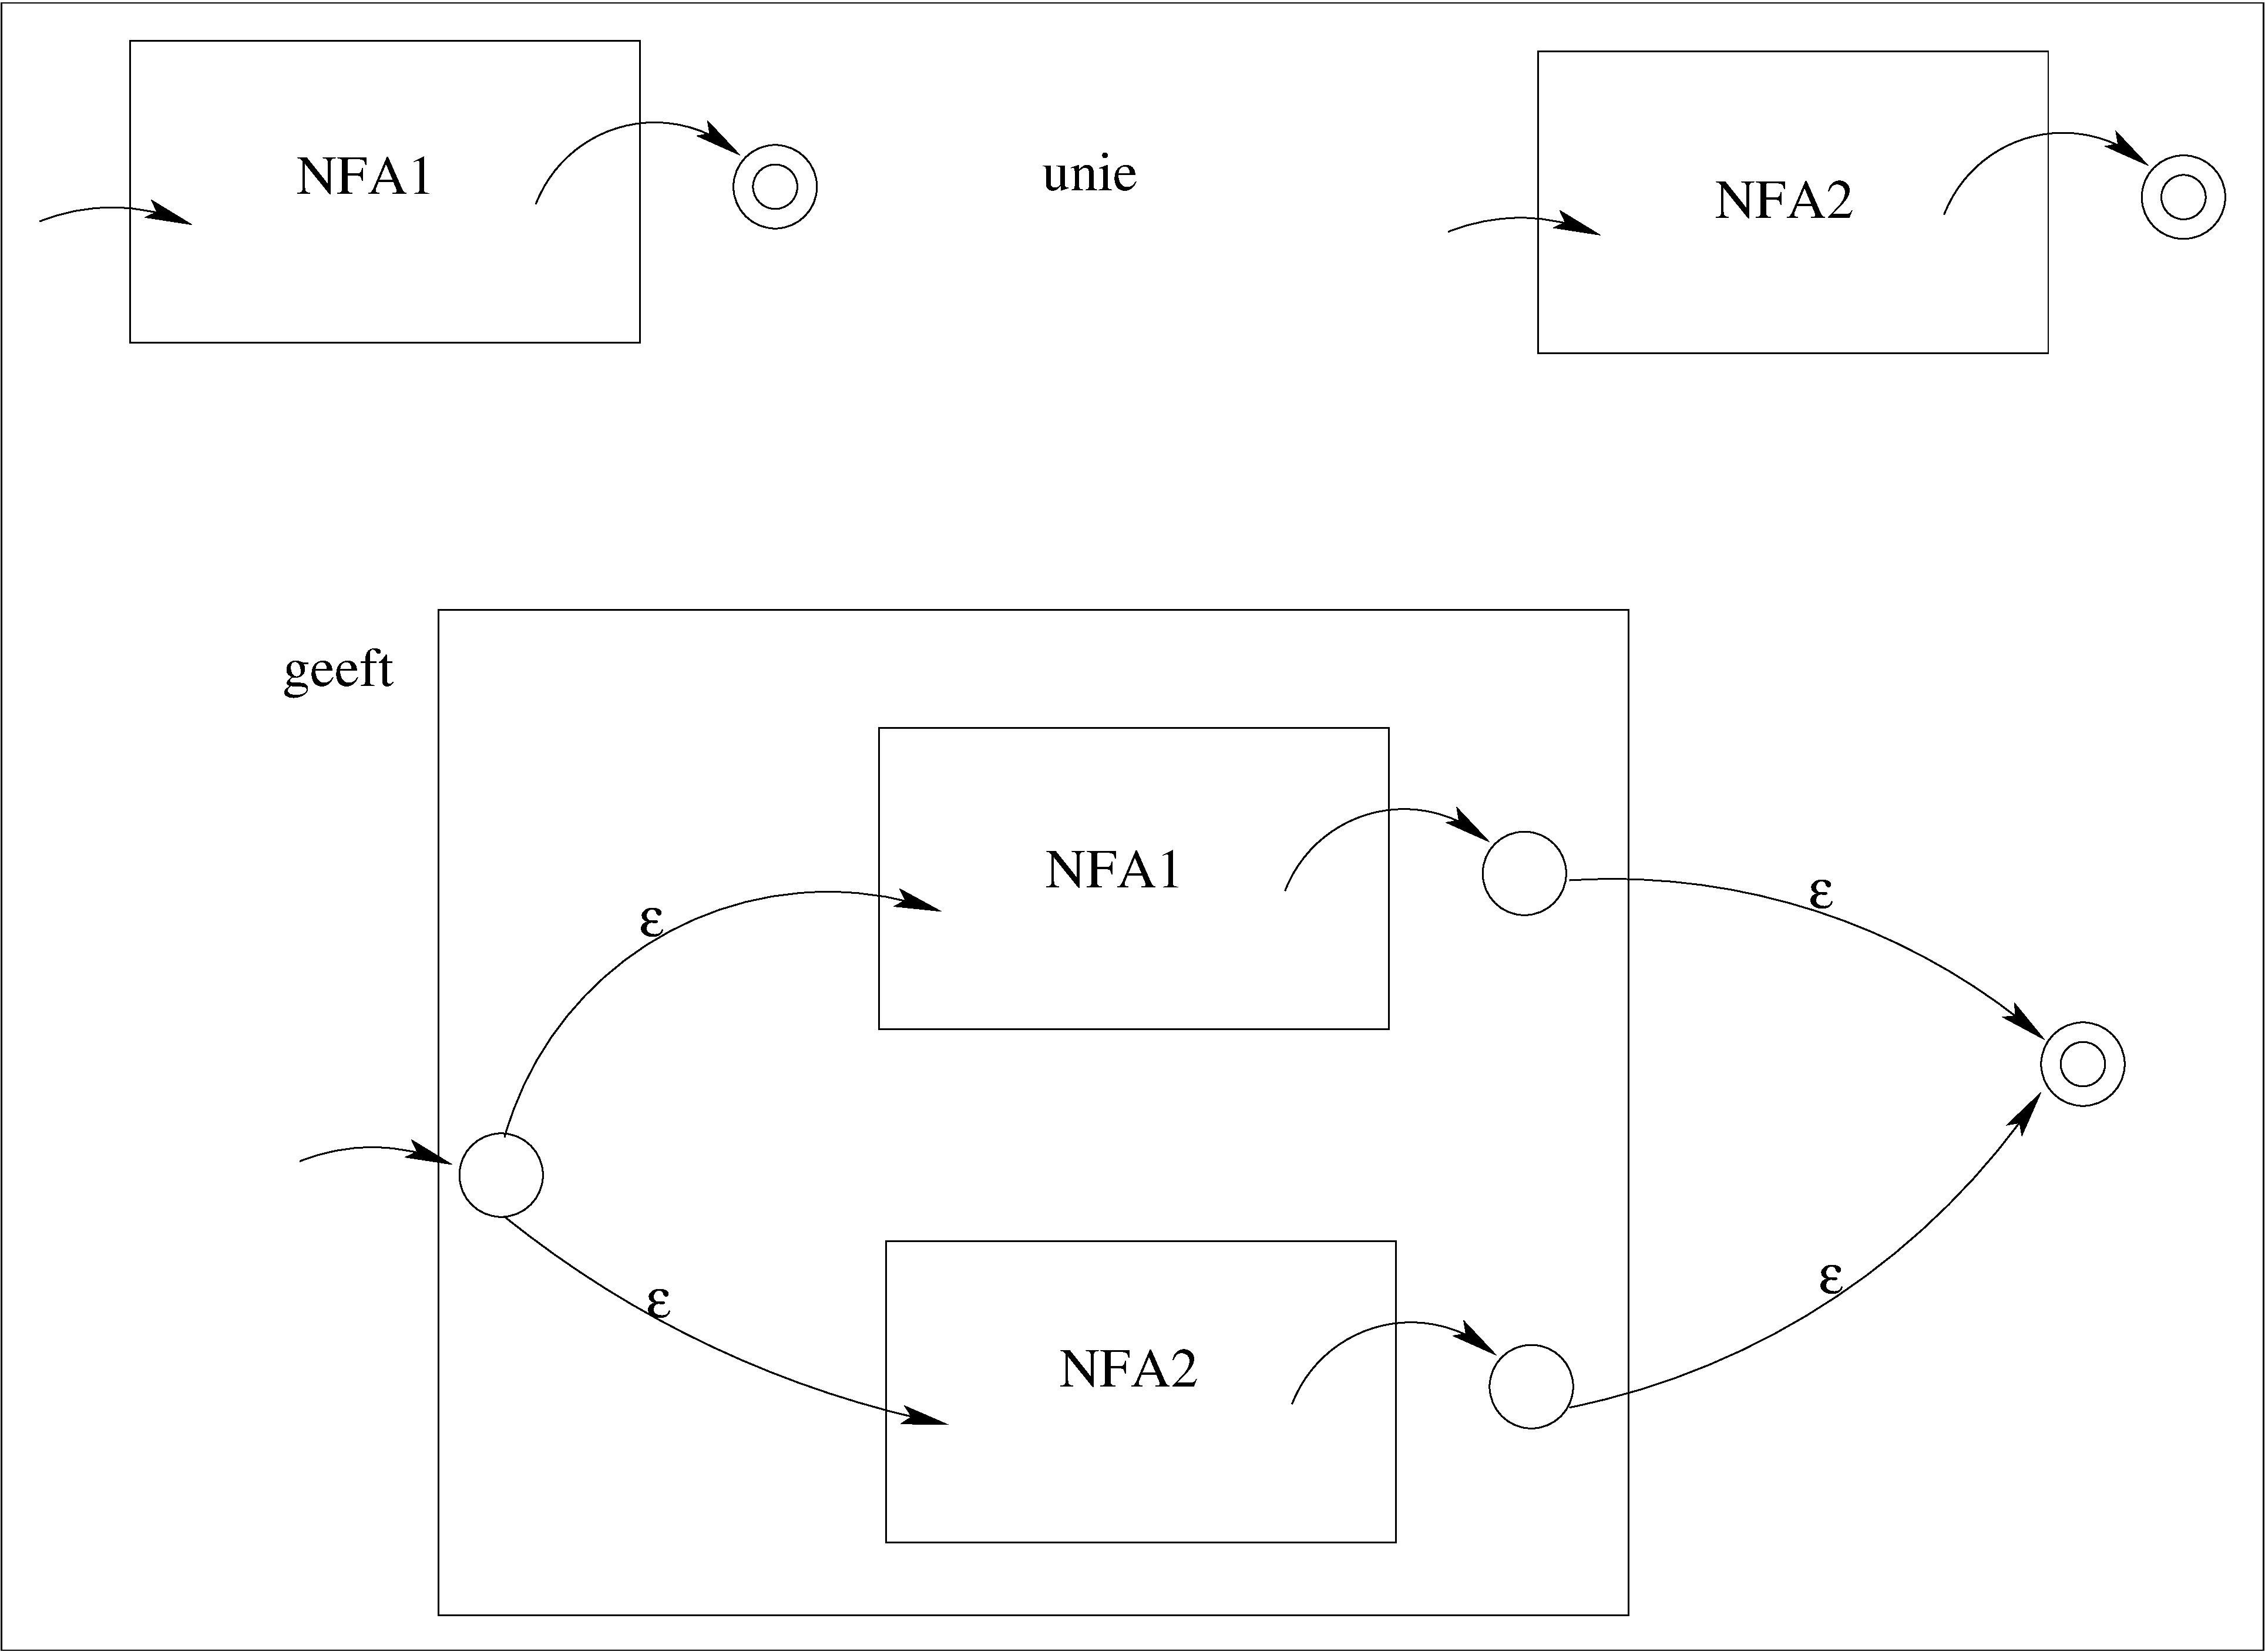
\includegraphics[%
  width=0.6\linewidth,
  keepaspectratio]{uniefsa}\end{center}
\caption{Unie van twee NFA's\label{uniefsa}}
\end{figure}


Formeel schrijven we:

Gegeven $NFA_1 = (Q_1,\Sigma,\delta_1,q_{s1},\{q_{f1}\})$ en 
%
$NFA_2 = (Q_2,\Sigma,\delta_2,q_{s2},\{q_{f2}\})$.

De unie $NFA_1 \cup NFA_2$ is de $NFA = (Q,\Sigma,\delta,q_s,F)$
waarbij
\begin{itemize}
\item $Q = Q_1 \cup Q_2 \cup \{q_s,q_f\}$ waarbij $q_s$ en $q_f$
nieuwe toestanden zijn
\item $F = \{q_f\}$
\item $\delta$ is gedefinieerd als:

 $\delta(q,x) = \delta_i(q,x)~~\forall q \in Q_i \backslash \{q_{fi}\}, x \in \Sigma_\epsilon$ voor i=1,2 \\
 $\delta(q_s,\epsilon) = \{q_{s1}, q_{s2}\}$ \\
 $\delta(q_s,x) = \emptyset ~~\forall x \in \Sigma$ \\
 $\delta(q_{fi},\epsilon) = \{q_f\}$ voor i = 1,2 \\
 $\delta(q_{fi}, x) = \emptyset ~~\forall x \in \Sigma$ en voor i = 1,2
\end{itemize}


\paragraph{De concatenatie van twee NFA's:} Deze keer geven we alleen
de visuele representatie van de concatenatie in Figuur~\ref{concatfsa}:

\begin{figure}[h]
\begin{center}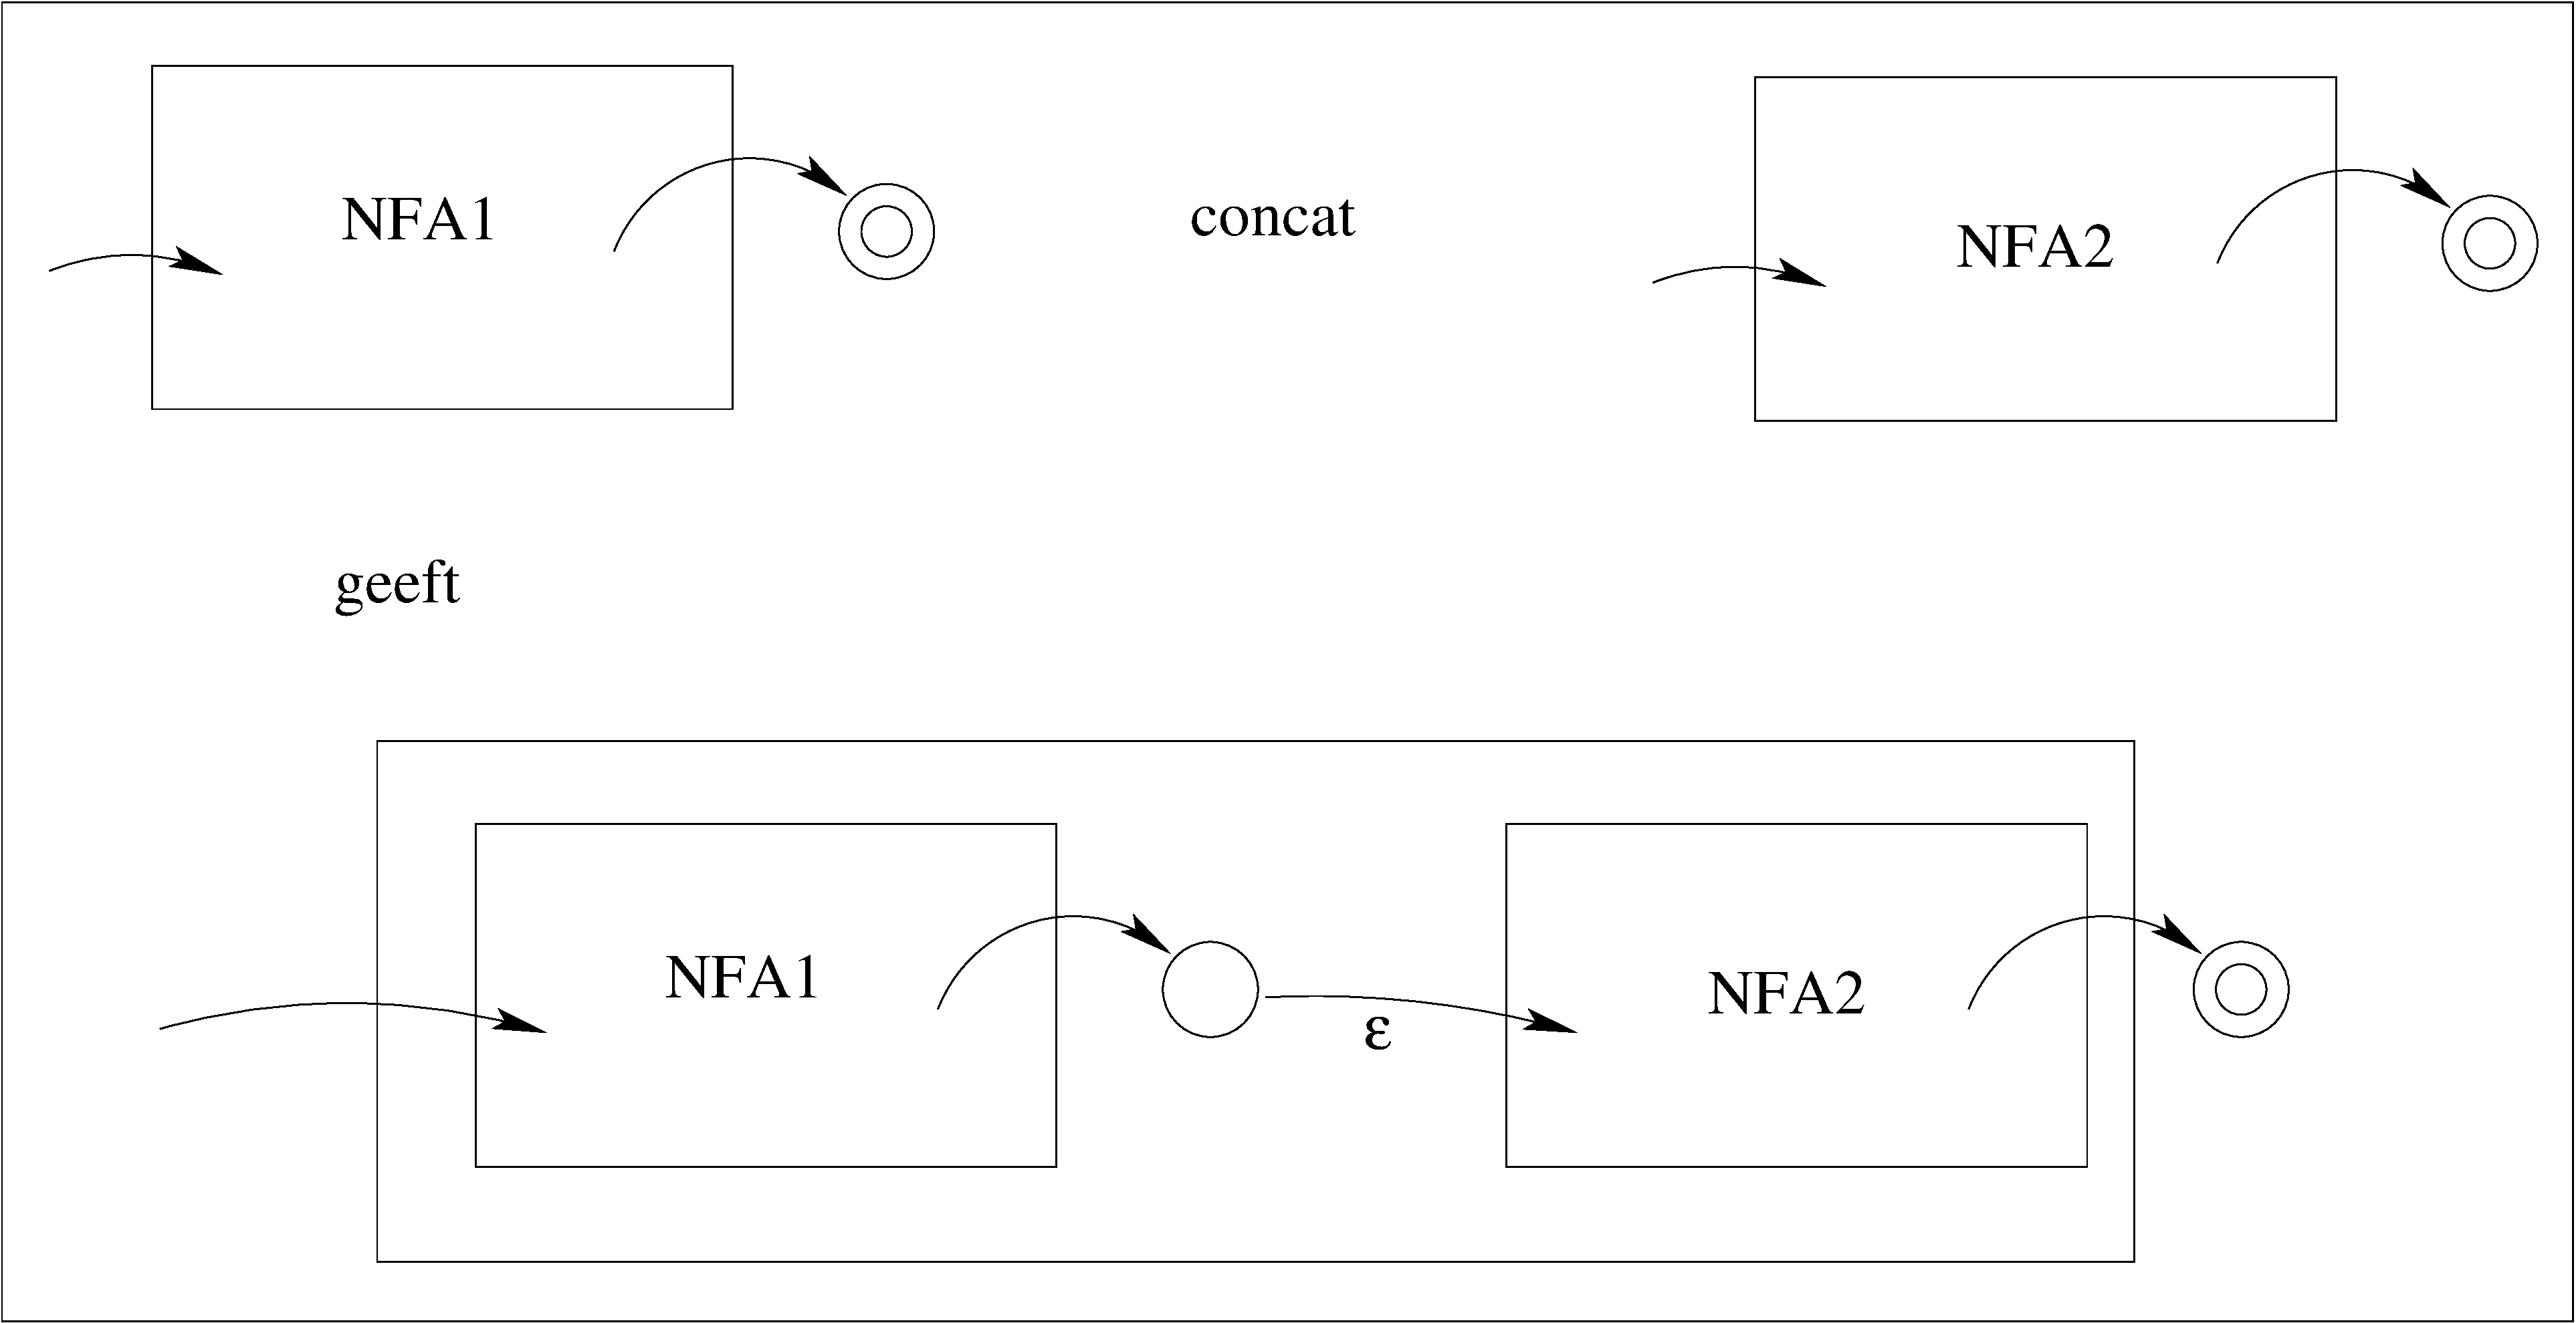
\includegraphics[%
  width=0.6\linewidth,
  keepaspectratio]{concatfsa}\end{center}
\caption{Concatenatie van twee NFA's\label{concatfsa}}
\end{figure}

\clearpage
\paragraph{De ster van een NFA:} weerom geven we enkel de visuele
representatie, in Figuur~\ref{starfsa}.

\begin{figure}[h]
\begin{center}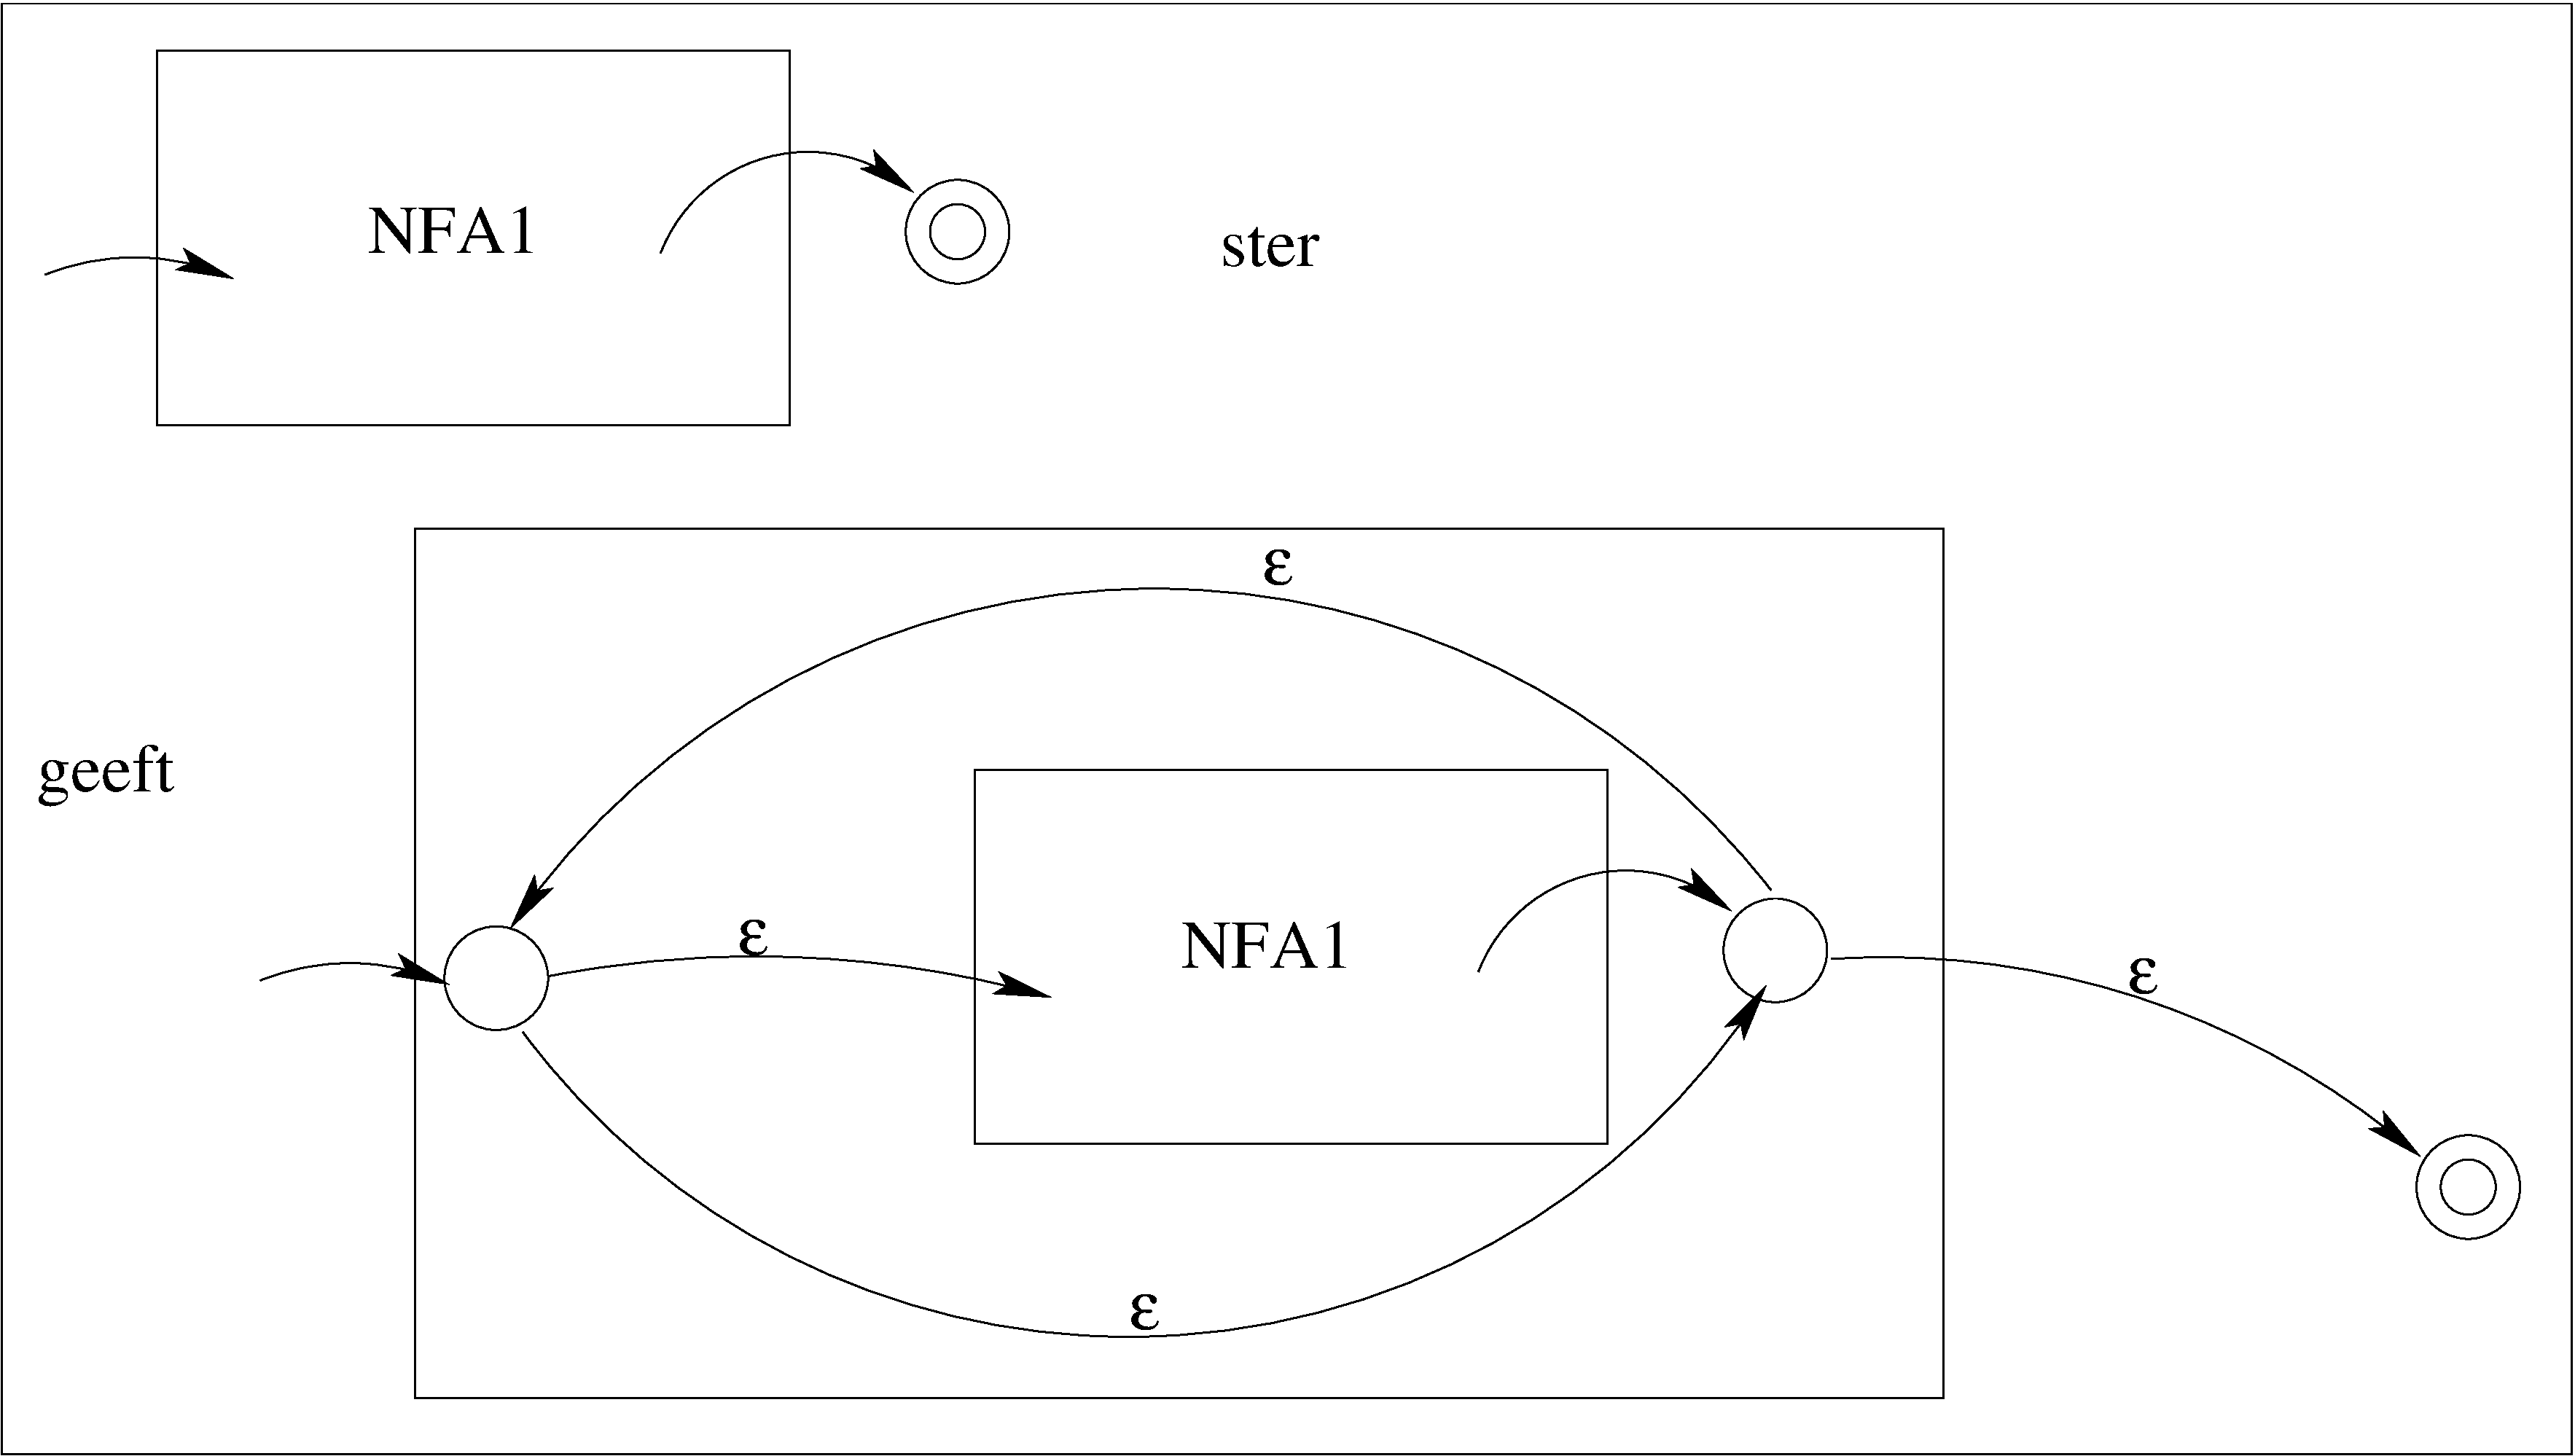
\includegraphics[%
  width=0.6\linewidth,
  keepaspectratio]{sterfsa}\end{center}
\caption{De ster van een NFA\label{starfsa}}
\end{figure}


Werk de formele beschrijvingen van concatenatie en de ster zelf uit.

\paragraph{Zelf doen:}
\begin{itemize}
\item[]
De concatenatie van $NFA_1$ en $NFA_2$ bepaalt
$L_{NFA_1}L_{NFA_2}$. Bewijs dat.

Formuleer iets analoogs voor de ster
en de unie.

Wat bewijst dat over de algebra\"{i}sche isomorfie tussen ... en ...?
\end{itemize}

\clearpage

\section{Van reguliere expressie naar NFA}\label{re2fsasec}

We hebben alle ingredi\"enten om van een reguliere expressie RE een NFA te
maken, en zodanig dat de $L_{RE} = L_{NFA}$. Vermits reguliere
expressies inductief gedefinieerd zijn (zie definitie pagina
\pageref{defregexp}) zullen we voor elk lijntje van die definitie een
overeenkomstige NFA defini\"eren. We gebruiken de notatie $NFA_{RE}$ om
de NFA aan te duiden die overeenkomt met de reguliere expressie RE.

Figuur~\ref{re2fsa} geeft de NFA voor de eerste drie basisgevallen in
de definitie op pagina \pageref{defregexp}:

\begin{figure}[h]
\begin{center}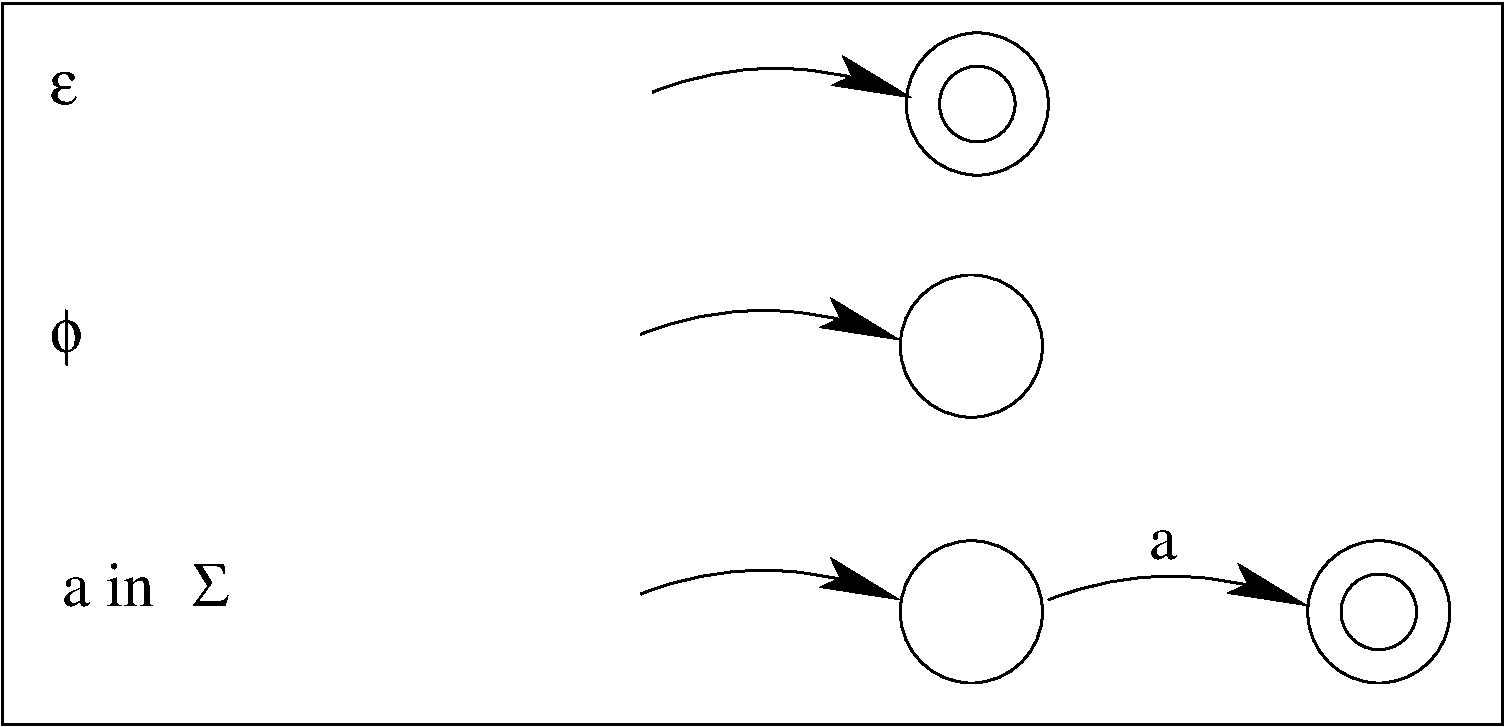
\includegraphics[%
  width=0.55\linewidth,
  keepaspectratio]{re2fsa}\end{center}
\caption{Een NFA voor de drie basisgevallen\label{re2fsa}}
\end{figure}

De drie recursieve gevallen beschrijven we als volgt: laat $E_1$ en
$E_2$ twee reguliere expressies zijn, dan is
\begin{itemize}
\item $NFA_{E_1E_2} = concat(NFA_{E_1},NFA_{E_2})$
\item $NFA_{E_1^*} = ster(NFA_{E_1})$
\item $NFA_{E_1|E_2} = unie(NFA_{E_1},NFA_{E_2})$
\end{itemize}

\grijs{\begin{stelling}  

De constructie hierboven bewaart de taal, t.t.z. 

~~~~~~~~~~~~~~~~~~~~~~~~~~~~ $L_{NFA_E} = L_E$.
\end{stelling}}
\begin{proof}
Geef zelf een bewijs door structurele inductie.
\end{proof}


\clearpage
\section{Van NFA naar reguliere expressie}

De weg omgekeerd is iets meer complex: we voeren eerst een nieuwe
soort van eindige automaten in - de GNFA's, de G staat voor
gegeneraliseerd. Daarna zullen we het volgende traject doorlopen:


$NFA \rightarrow GNFA \rightarrow GNFA~met~2~toestanden \rightarrow reguliere~expressie$


In elk van die stappen zullen we hard moeten maken dat de taal beschreven
door het formalisme niet verandert.

\grijs{\begin{informeledefinitie} GNFA\\
{\rm
Een {\bf GNFA} is een eindige toestandsmachine met de volgende
wijzigingen en beperkingen:
\begin{itemize}
\item er is slechts \'{e}\'{e}n eindtoestand en die is verschillend
van de starttoestand
\item er is juist \'{e}\'{e}n boog van de starttoestand naar elke
andere toestand, maar er komen geen pijlen aan (behalve de startpijl)
\item er is juist \'{e}\'{e}n boog van elke toestand naar de
eindtoestand maar uit de eindtoestand vertrekken geen pijlen
\item tussen elke andere twee toestanden is er juist \'{e}\'{e}n boog
in beide richtingen
\item er is ook juist \'{e}\'{e}n boog van elke andere toestand naar
zichzelf
\item de bogen hebben als label een reguliere expressie
\end{itemize}
}
\end{informeledefinitie}}

% \clearpage 
Figuur~\ref{gfsa1} toont een GNFA.

\begin{figure}[h]
\begin{center}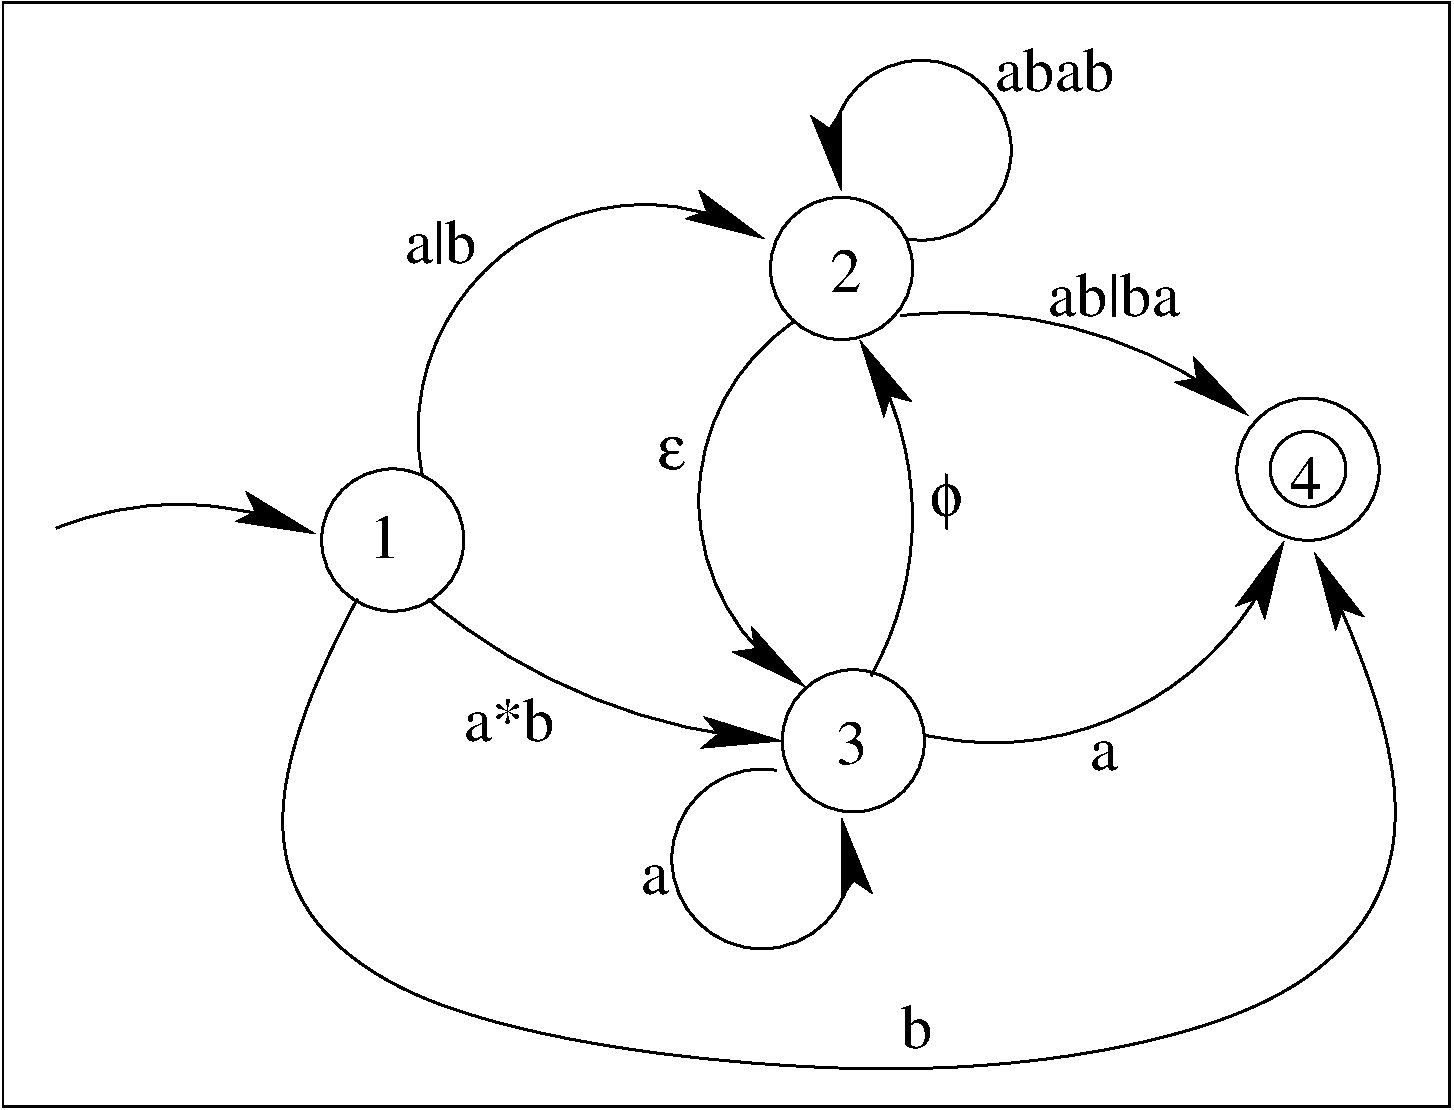
\includegraphics[%
  width=0.5\linewidth,
  keepaspectratio]{gfsa1}\end{center}
\caption{Een GNFA\label{gfsa1}}
\end{figure}

We gebruiken de (grafische voorstelling van de) GNFA als volgt:

\begin{enumerate}
\item je krijgt een string $s$ over het alfabet en vertrekt ermee in
de starttoestand
\item je mag nu van \'{e}\'{e}n toestand naar een andere overgaan door
een boog te volgen en in je vertrektoestand een rij symbolen die van
voor op je string voorkomen achter te laten; die rij symbolen moet
voldoen aan de reguliere expressie die op de boog staat; je string wordt
daardoor korter; als de boog ook $\epsilon$ bevat, dan hoef je niet
een teken achter te laten; als de boog enkel maar $\phi$ bevat, dan
kan je de boog niet nemen
\item blijf overgangen maken: als je aankomt in de eindtoestand en
je string is leeg op dat ogenblik, dan zeggen we {\em de GNFA heeft de
initi\"ele string $s$ aanvaard}
\end{enumerate}

% \newpage
\paragraph{Zelf doen:}
\begin{itemize}
\item[]
Zoek voor de GNFA in Figuur~\ref{gfsa1} strings
die aanvaard worden en strings die niet aanvaard worden.
\end{itemize}


% \clearpage
We beschrijven nu een algoritme om van een gegeven NFA een RE te maken:

\begin{itemize}
\item[Stap 1:]  {\em Maak van de NFA een GNFA} 

Voer een nieuwe starttoestand in en een nieuwe (unieke)
eindtoestand. Teken een $\epsilon$-boog van de nieuwe begintoestand naar
de oude begintoestand, en van elke oude eindtoestand naar de
nieuwe eindtoestand. Teken de ontbrekende bogen met een $\phi$.
Als er nu tussen twee toestanden twee of meer parallelle gerichte
bogen zijn, neem die dan samen met als label de unie van de labels van
de parallelle bogen.

\item[Stap 2:]  {\em Reduceer de GNFA}

Kies een willekeurige toestand X verschillend van de start- of
eindtoestand - als er geen meer zijn, ga naar stap 3. Verwijder die
knoop als volgt: kies toestanden A en B zodat er bogen zijn van A naar
B met label $E_4$, van A naar X met $E_1$, van X naar zichzelf met
$E_2$ en van X naar B met $E_3$. Vervang het label op de boog van A
naar B door $E_4~|~E_1E_2^*E_3$. Doe dit voor alle koppels A en
B. Verwijder daarna de knoop X met alle bogen die erin toekomen of
vertrekken.

De basisstap wordt ge\"{i}llustreerd in Figuur~\ref{redgfsa1}.

\begin{figure}[h]
\begin{center}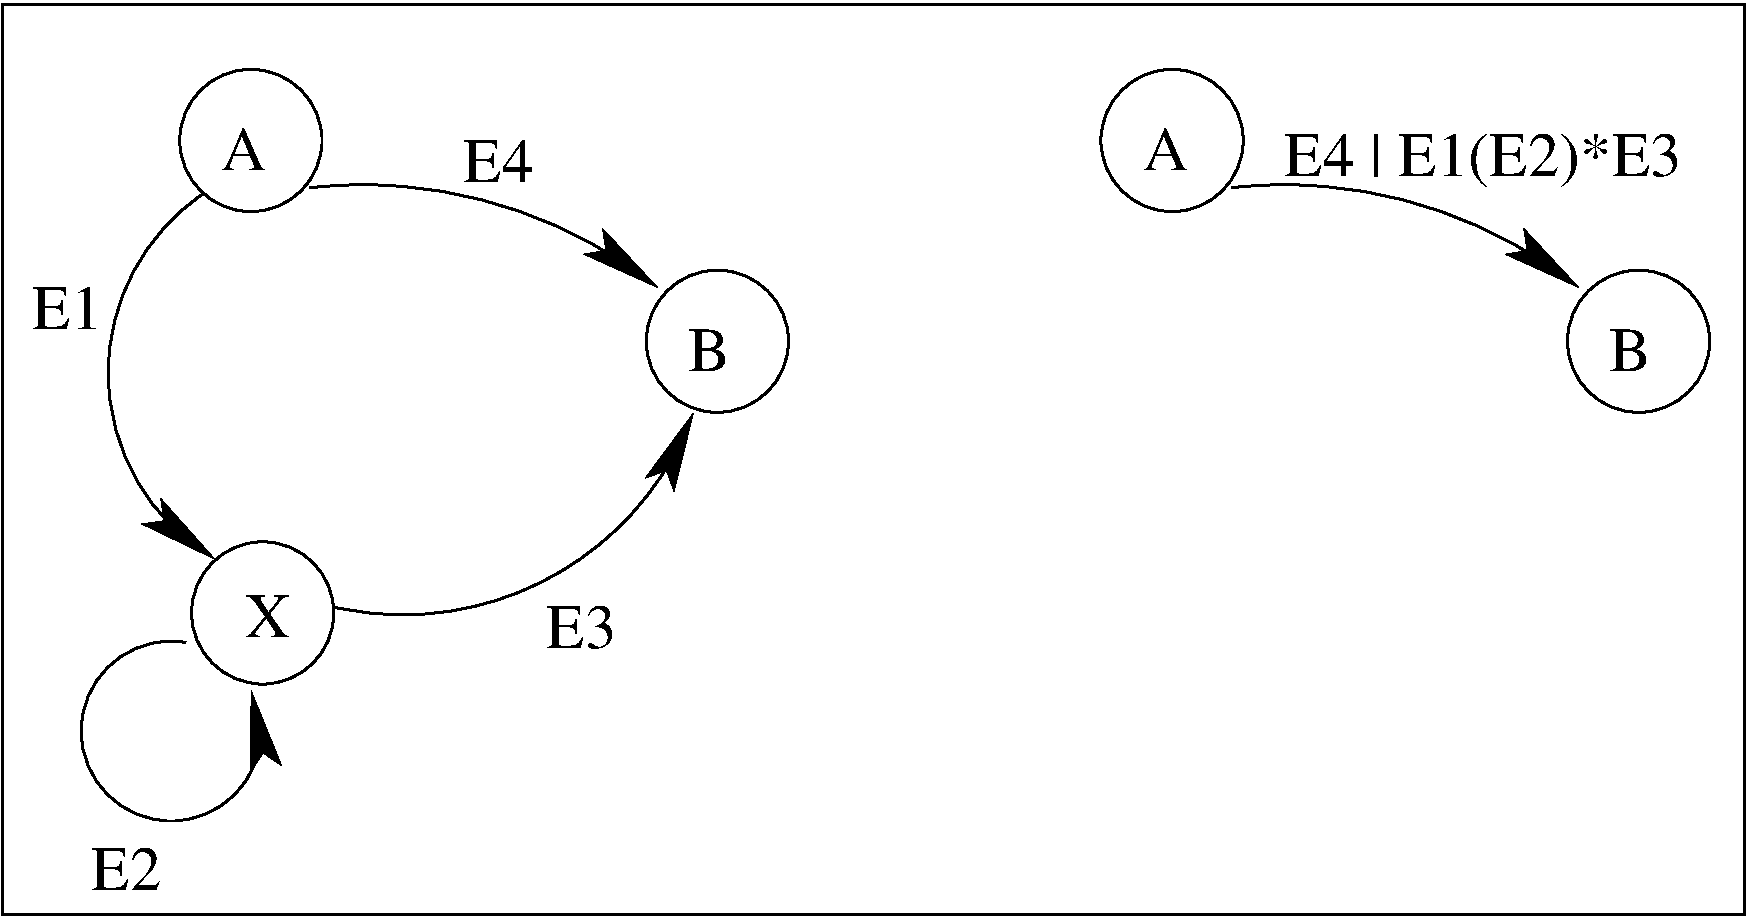
\includegraphics[%
  width=0.6\linewidth,
  keepaspectratio]{redgfsa1}\end{center}
\caption{Verwijdering van \'{e}\'{e}n toestand uit een GNFA \label{redgfsa1}}
\end{figure}

Herhaal stap 2.


\item[Stap 3:]  {\em Bepaal RE}

De GNFA heeft nu juist 2 toestanden (start- en eindtoestand) en
daartussen \'{e}\'{e}n boog; die boog heeft een RE als label; dit is
de RE die we zochten.
\end{itemize}

% \clearpage
\paragraph{Voorbeeld:} We passen dit stapsgewijze toe op de GNFA van
Figuur~\ref{gfsa1}: Figuren~\ref{gfsa2}~en~\ref{gfsa3} tonen dat.


\begin{figure}[h]
\begin{center}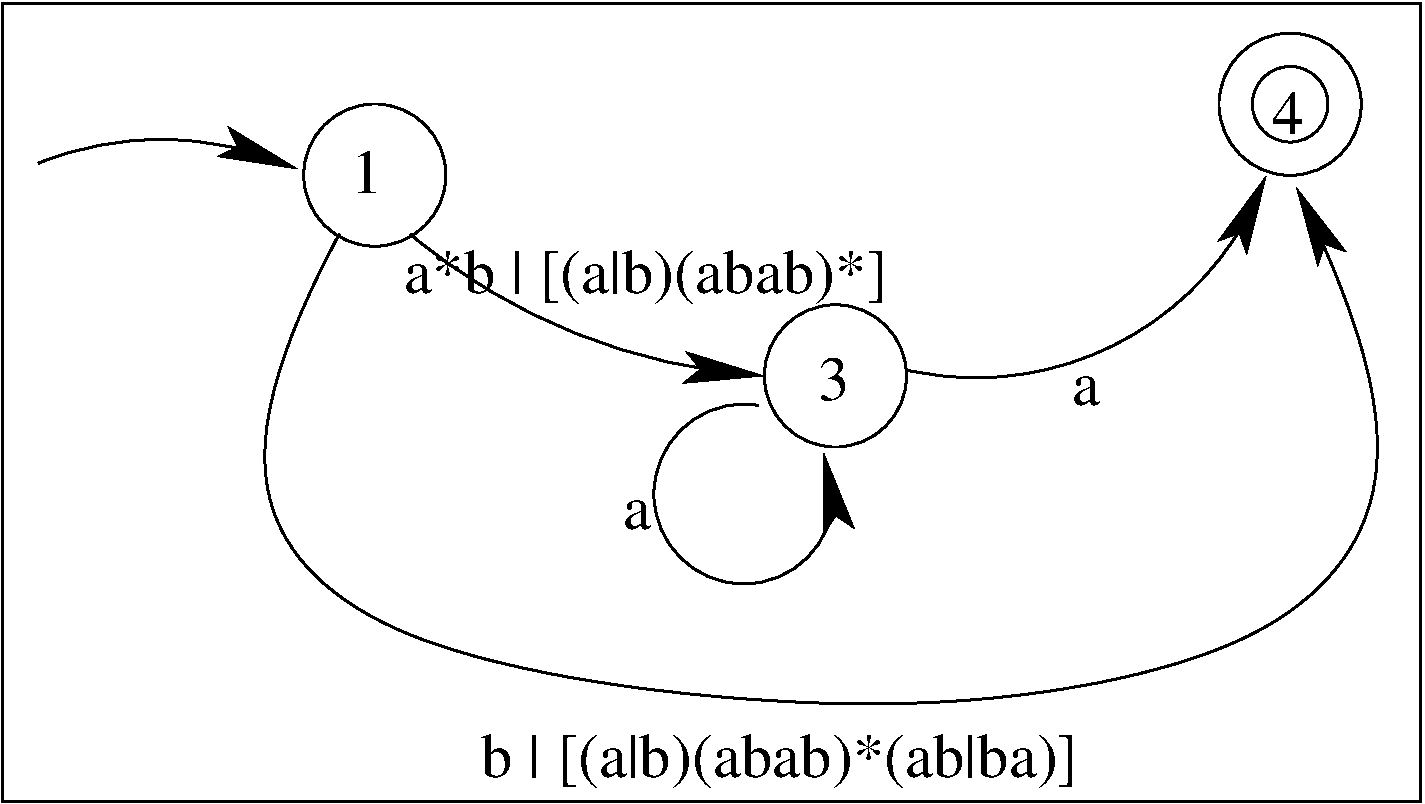
\includegraphics[%
  width=0.6\linewidth,
  keepaspectratio]{gfsa2}\end{center}
\caption{Toestand 2 is verwijderd \label{gfsa2}}
\end{figure}

\begin{figure}[h]
\begin{center}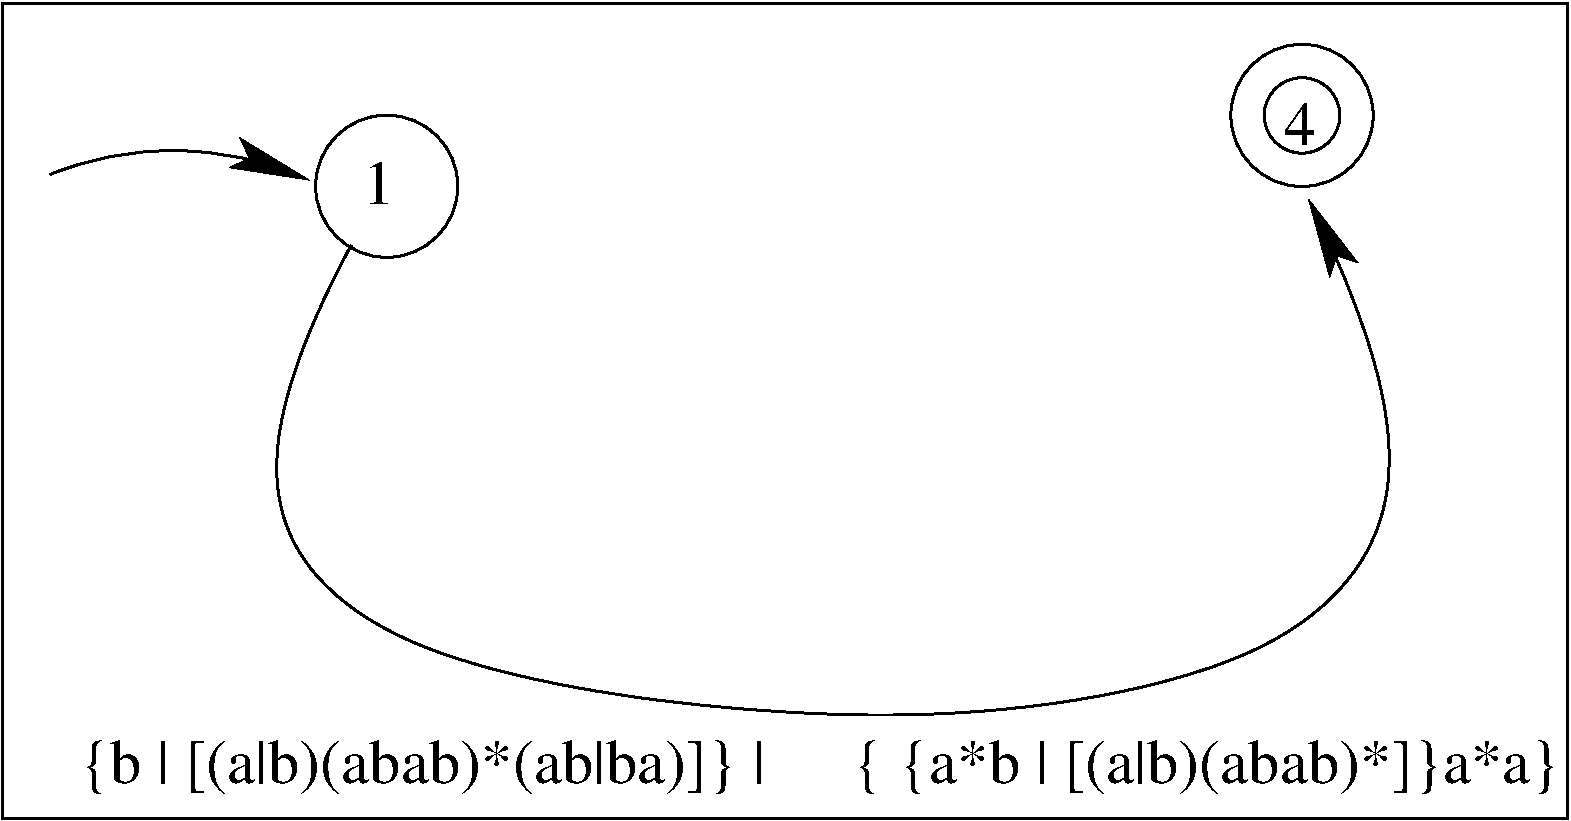
\includegraphics[%
  width=0.6\linewidth,
  keepaspectratio]{gfsa3}\end{center}
\caption{Toestand 3 is verwijderd\label{gfsa3}}
\end{figure}


We moeten nog bewijzen dat de reductie met \'{e}\'{e}n toestand in
Stap 2 in het algoritme de verzameling aanvaarde strings niet
verandert. We moeten daarvoor twee dingen bewijzen: (1) indien een
string s aanvaard werd voor de reductie, dan ook na de reductie; (2)
indien een string s niet aanvaard werd voor de reductie, dan ook niet
na de reductie.

\newpage
We gebruiken de notie van het pad doorheen de toestanden dat je kan
volgen om een string te accepteren (die notie staat voor een NFA in de
definitie op pagina \pageref{defacceptnfa} - schrijf ze hier eens uit
voor een GNFA): zulk een acceptatiepad is dus een opeenvolging van
toestanden. We verwijzen naar de machine voor de reductie met
$GNFA_{voor}$ en naar de machine erna met $GNFA_{na}$.

\begin{enumerate}
\item
Als s aanvaard werd door $GNFA_{voor}$ met een pad dat X niet bevat,
dan wordt s door datzelfde pad in $GNFA_{na}$ aanvaard.

Als dat pad X bevat, dan zijn er toestanden A en B, zodat AX$^n$B
($n>0$) een opeenvolging is in het pad. De reguliere expressies op de
bogen AX, XX, XB zijn E1, E2, E3 en bijgevolg kost van A naar B gaan
langs X een stukje string dat voldoet aan $E1(E2)^*E3$: die reguliere
expressie staat ook in de boog AB in $GNFA_{na}$, dus ...

\item
Als s aanvaard wordt door $GNFA_{na}$ dan bevat het acceptatiepad
uiteraard alleen maar toestanden verschillend van X. Op een boog van A
naar B (twee opeenvolgende toestanden in het acceptatiepad) staat de
reguliere expressie $E4 | E1(E2)^*E3$: die gebruiken betekent een
stukje string uitgeven dat voldoet aan E4 of aan $E1(E2)^*E3$, dus in
$GNFA_{voor}$ komt dat overeen met ofwel de boog AB volgen ofwel de
bogen AX, XX (zo dikwijls als nodig) en XB. AB had als label
$E4$, AX heeft E1, ... 

Dus als een string aanvaard wordt door $GNFA_{na}$ dan ook door
$GNFA_{voor}$.

\end{enumerate}

We moeten ook nog stap 1 verantwoorden, t.t.z. argumenteren dat door
de NFA om te vormen naar een GNFA, de taal niet verandert. Doe dat zelf.


\paragraph{Besluit:} twee formalismen (NFA en RE) bepalen precies
dezelfde klasse van talen die we de reguliere talen hebben genoemd. We
hebben dat bewezen en de bewijzen zijn constructief: we kunnen de
bewijzen gemakkelijk omvormen tot programma's in Java, Prolog ... om
vanuit een RE een NFA te berekenen, of omgekeerd. We kunnen echter
beter doen dan tot nu toe: onze NFA's zijn niet-deterministisch en het
zou leuk zijn als we genoeg hebben aan deterministische automaten. In
Sectie~\ref{detfsa} zullen we dit uitspitten. Tenslotte kunnen we
ook een minimaliteitscriterium voor deterministische automaten
bestuderen: dat gebeurt in Sectie~\ref{minfsa}.






\section{Deterministische eindige toestandsmachines}\label{detfsa}

De definitie van een eindige toestandsmachine NFA laat toe dat vanuit een
bepaalde toestand bogen vertrekken met $\epsilon$ en ook meer dan
\'{e}\'{e}n boog met (bijvoorbeeld) het label $a$ ($a$ in het
alfabet). Dat is de bron van niet-determinisme: als in die toestand
het eerste symbool van je huidige string $a$ is, dan heb je de keuze: $a$
achterlaten en nog keuze tussen welke boog met $a$ erop volgen, of niets
achterlaten en de $\epsilon$-boog volgen. Dit implementeren
(bijvoorbeeld op basis van de transitietabel) is niet moeilijk, maar
als je alle mogelijkheden wil uitproberen, dan moet je op je stappen
kunnen terugkeren. Ook weer niet onoverkomelijk, maar het is duidelijk
dat dit niet tot optimale programma's zal leiden. Het ware effici\"enter
als er in elke toestand slechts \'{e}\'{e}n mogelijkheid bestond per
symbool en geen \eps-overgangen. We beperken dus de klasse van
automaten tot de deterministische eindige toestandsmachines - we
noteren DFA - door geen $\epsilon$-overgangen toe te laten en
bovendien mag een symbool van het alfabet hoogstens op \'{e}\'{e}n
uitgaande boog per toestand staan. Formeel doen we dat door te
schrijven dat $\delta : Q \times \Sigma \rightarrow Q$ een parti\"ele
functie is. Het zou moeten duidelijk zijn dat een taal bepaald door een
DFA ook regulier is.  De volgende vraag is daarmee nog niet
beantwoord: kan elke reguliere taal bepaald worden door een DFA?  

Een andere manier om daar tegenaan te kijken is de volgende: gegeven
een reguliere taal L, dan bestaat er een reguliere expressie E voor L;
voor die E kunnen we gemakkelijk de automaat $NFA_E$ maken (zie pagina
\pageref{re2fsasec}). Laat ons nu proberen die $NFA_E$ om te vormen
tot een DFA die dezelfde taal (L) aanvaardt. Als dat lukt hebben we
bewezen dat elke reguliere taal door een DFA bepaald wordt.


We beschrijven de transformatie van een NFA naar de DFA in het algemeen.

\clearpage

\begin{itemize}
\item[{\bf Gegeven:}] een NFA = $(Q_n,\Sigma,\delta_n,q_{sn},F_n)$

\item[{\bf Gevraagd:}] een DFA = $(Q_d,\Sigma,\delta_d,q_{sd},F_d)$ zodanig dat
$L_{NFA} = L_{DFA}$

\item[{\bf Constructie:}] 
$Q_d = {\cal P}(Q_n)$: elke toestand in de DFA is een verzameling
toestanden van de NFA

$F_d = \{S |S \in Q_d, S \cap F_n \neq \emptyset\}$: een eindtoestand
in de DFA bevat altijd een eindtoestand van de NFA

Dat laat ons nog $\delta_d$. Voor de duidelijkheid: 
%
$\delta_d :  ({\cal P}(Q_n) \times \Sigma) \rightarrow {\cal P}(Q_n)$


We voeren eerst een afbeelding $eb : Q_n \rightarrow {\cal P}(Q_n)$ in
(eb staat voor {\bf e}psilon-{\bf b}ereikbaar):

\begin{itemize}
\item $eb(q)$ is de verzameling toestanden in NFA die met nul,
\'{e}\'{e}n of meer $\epsilon$-bogen bereikbaar zijn vanuit q

\item 
We liften de definitie van eb naar ${\cal P}(Q_n)$ op de gewone
manier: voor een ${\cal Q} \in {\cal P}(Q_n)$

$~~~~~~~~~~~~~~~~~eb({\cal Q}) = \cup_{q \in {\cal Q}} eb(q)$

\item 
 $\delta_n$ liften we op dezelfde manier.
\end{itemize}



Vervolgens defini\"eren we $\delta_d$ als volgt:
\begin{itemize}
\item 
$\delta_d({\cal Q},a) = eb(\delta_n({\cal Q},a))$ \footnote{Kijk de
signatuur na!} voor ${\cal Q} \in Q_d$

\item 
in woorden: vanuit een toestand ${\cal Q}$ in de DFA ga je naar een
volgende toestand in de DFA door voor elke NFA toestand in ${\cal Q}$
eerst de overgangsfunctie van de NFA te gebruiken, en daarna de
$\epsilon$-bogen te volgen - van al die resulterende
toestandsverzamelingen neem je de unie.

\end{itemize}



Tenslotte defini\"eren we


$~~~~~~~~~~~~~~~~q_{sd} = eb({q_{sn}})$.


\item[{\bf Einde}]
\end{itemize}


We passen die constructie toe op de NFA in Figuur~\ref{fsa2}. Die NFA
heeft 3 toestanden, dus hebben we in principe 8 toestanden in de
resulterende DFA.

\clearpage

\begin{figure}[h]
\begin{center}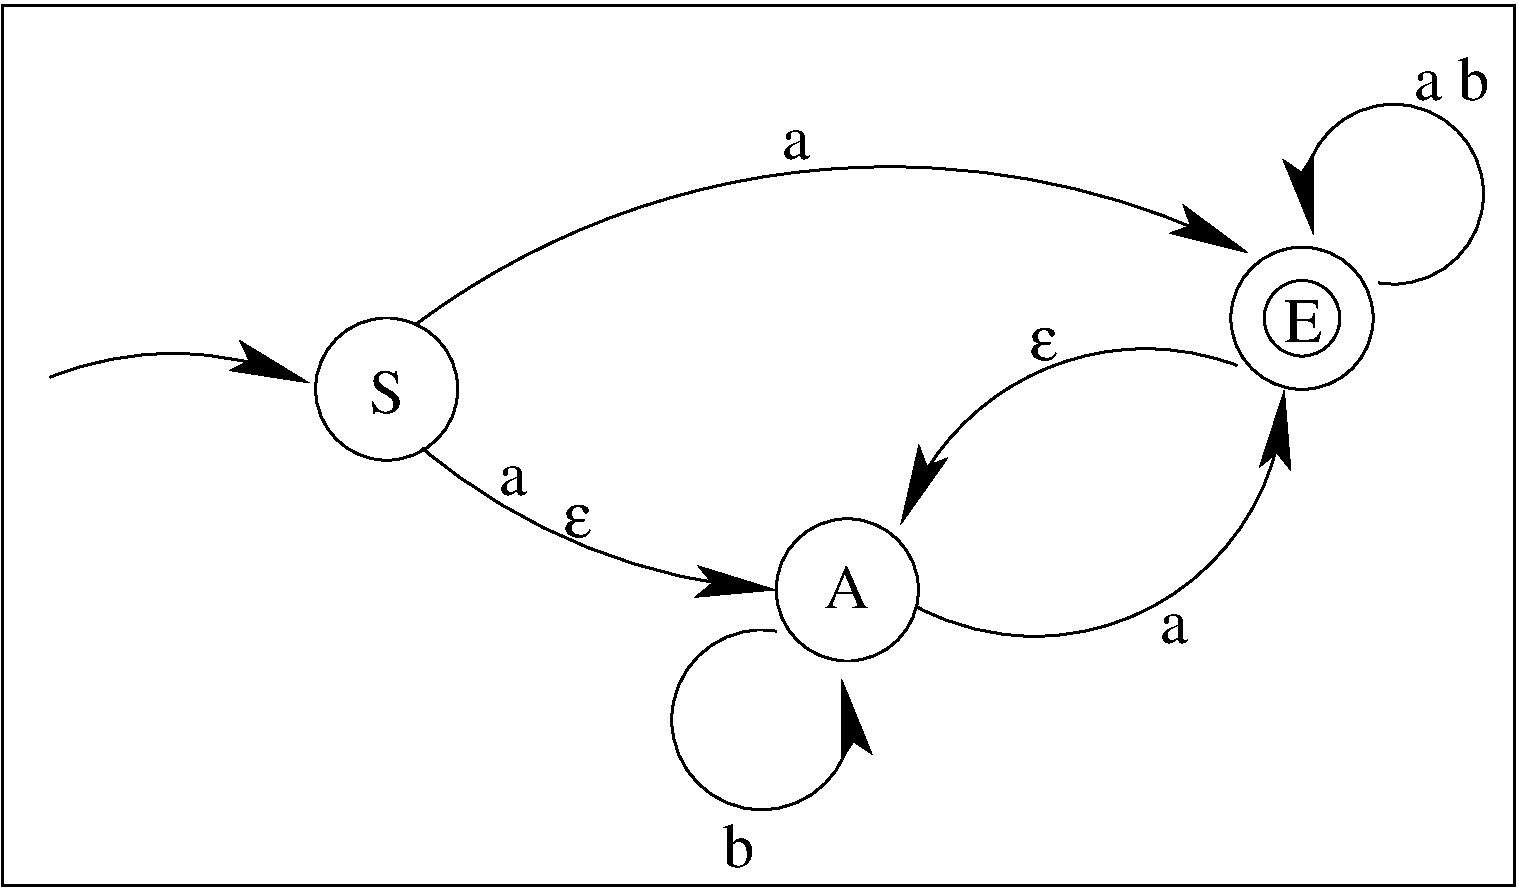
\includegraphics[%
  width=0.6\linewidth,
  keepaspectratio]{fsa2}\end{center}
\caption{Een NFA \label{fsa2}}
\end{figure}


Tabel~\ref{charstable} laat het resultaat zien van de constructie van
de verschillende onderdelen van de DFA. 


\begin{table}[ht]
\center
\begin{tabular}{|r|r|r|r|r|r|}
\hline
$q \in Q_d$    & $eb(q)$  &  $\delta_n(q,a) $ & $\delta_n(q,b) $ & $\delta_d(q,a)$ & $\delta_d(q,b)$ \\ \hline
\{\}           & \{\}     &  \{\}             & \{\}             & \{\}            & \{\}            \\
\{S\}          & \{S,A\}  &  \{A,E\}          & \{\}             & \{A,E\}         & \{\}            \\
\{A\}          & \{A\}    &  \{E\}            & \{A\}            & \{A,E\}         & \{A\}           \\
\{E\}          & \{A,E\}  &  \{E\}            & \{E\}            & \{A,E\}         & \{A,E\}         \\
\{S,A\}        & \{S,A\}  &  \{A,E\}          & \{A\}            & \{A,E\}         & \{A\}           \\
\{S,E\}        & \{S,A,E\}&  \{A,E\}          & \{E\}            & \{A,E\}         & \{A,E\}         \\
\{A,E\}        & \{A,E\}  &  \{E\}            & \{A,E\}          & \{A,E\}         & \{A,E\}         \\
\{S,A,E\}      & \{S,A,E\}&  \{A,E\}          & \{A,E\}          & \{A,E\}         & \{A,E\}         \\
\hline
\end{tabular}
\caption{De onderdelen van de DFA voor de NFA in Figuur~\ref{fsa2}} \label{charstable}
\end{table}


Een aantal toestanden is niet bereikbaar vanuit de starttoestand
$\{S,A\}$. Het is voldoende om enkel de bereikbare toestanden voor te
stellen: de grafische voorstelling van de DFA is te zien in figuur
\ref{fsa3}.

\clearpage
\begin{figure}[h]
\begin{center}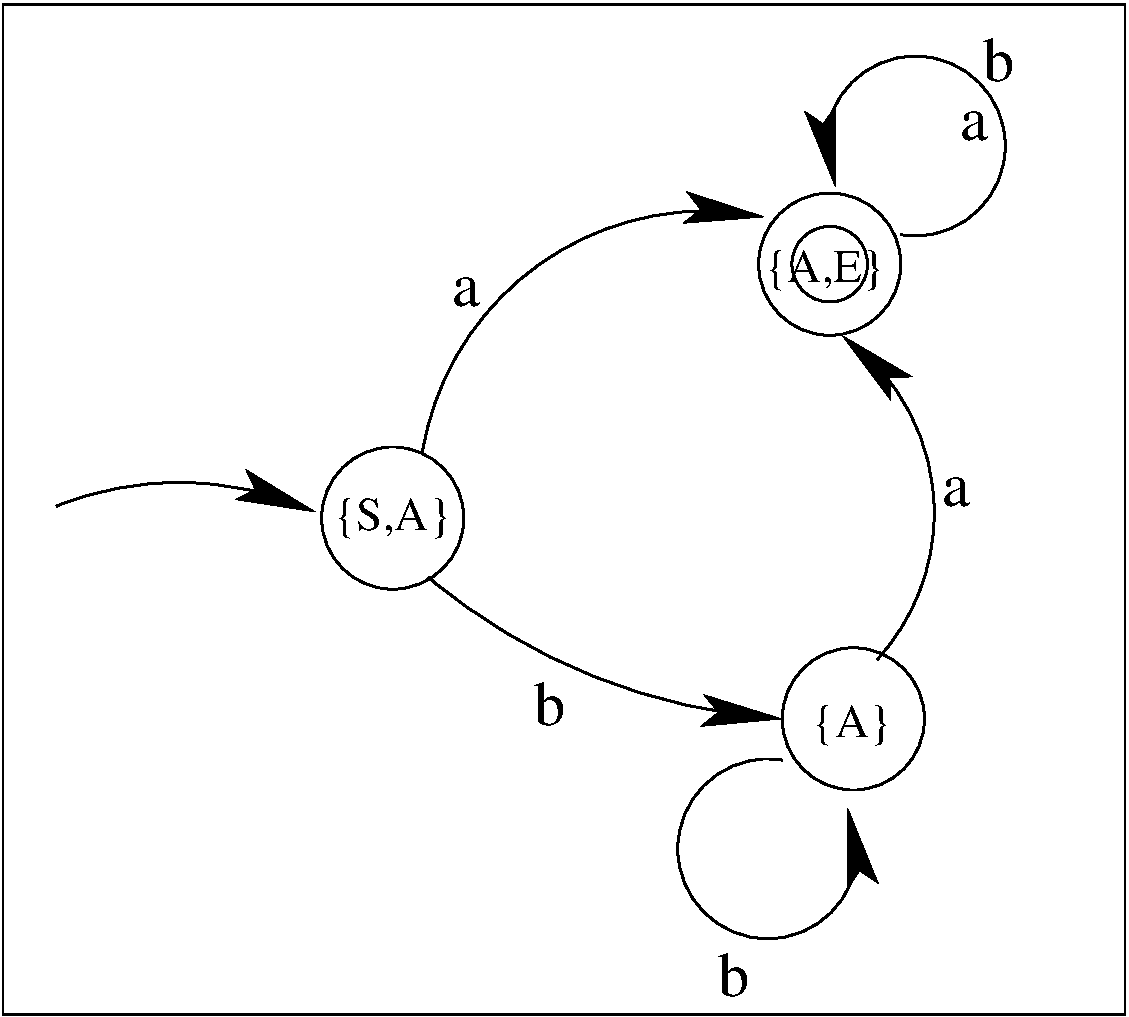
\includegraphics[%
  width=0.45\linewidth,
  keepaspectratio]{fsa3}\end{center}
\caption{De resulterende DFA \label{fsa3}}
\end{figure}

\paragraph{Zelf doen:}
\begin{itemize}
\item[]
Bepaal welke taal deze automaat beschrijft. Of maak er een reguliere
expressie van en druk dan in woorden uit welke strings aanvaard
worden. Is dit de {\em kleinste} automaat die deze taal bepaalt? Wat
is volgens jou een goede notie van {\em kleinste} automaat?


De constructie vereist maximaal $2^{\#Q_n}$ toestanden in de DFA, maar
het voorbeeld toont dat het voorkomt dat $Q_d$ niet veel groter hoeft
te zijn dan $Q_n$, als we de niet bereikbare toestanden niet opnemen.
Is het mogelijk dat de DFA {\em minder} toestanden heeft dan de NFA
waarvan we vertrokken?

\end{itemize}



\paragraph{Uitbreiding van $\delta$ naar strings:} voor een DFA heeft
$\delta$ als domein $Q \times \Sigma$. Het is handig $\delta$ uit te
breiden tot een functie $\delta^*$ op het domein $Q \times \Sigma^*$
als volgt:

\begin{itemize}
\item $\delta^*(q,\epsilon) = q$
\item $\delta^*(q,aw) = \delta^*(\delta(q,a),w)$ indien $\delta(q,a)$
bestaat - hierin is $a \in \Sigma$ en $w \in \Sigma^*$.
\end{itemize}

\paragraph{Zelf doen:}
\begin{itemize}
\item[]
Bewijs dat $\delta^*(q,wa) = \delta(\delta^*(q,w),a)$ voor $a \in
\Sigma$ en $w \in \Sigma_{\epsilon}^*$
\end{itemize}

\clearpage
\section{Minimale DFA}\label{minfsa}

Voor een gegeven reguliere taal L bestaan er meestal veel DFA's die de
taal bepalen\footnote{Soms oneindig veel?}. Het is belangrijk om
kleine machines te maken: als je in een toepassing een DFA nodig hebt,
dan moet je op een of andere manier de toestanden voorstellen en dus
heb je er belang bij het aantal toestanden laag te houden. Het is
zonder meer duidelijk dat er voor een gegeven reguliere taal een DFA
bestaat met het minimale aantal toestanden. De vraag is hoe we een
minimale DFA construeren, en bewijzen dat de constructie een minimale
DFA oplevert. We proberen minimaliteit te verkrijgen door toestanden
weg te halen uit de machine.


Toestanden die niet bereikbaar zijn vanuit $q_s$ zijn nutteloos: die
toestanden kunnen we zonder meer wegdoen.


Om nog meer toestanden weg te doen, eerst een voorbeeld: Figuur
\ref{mini1} toont links een DFA met 5 toestanden.

\begin{figure}[h]
\begin{center}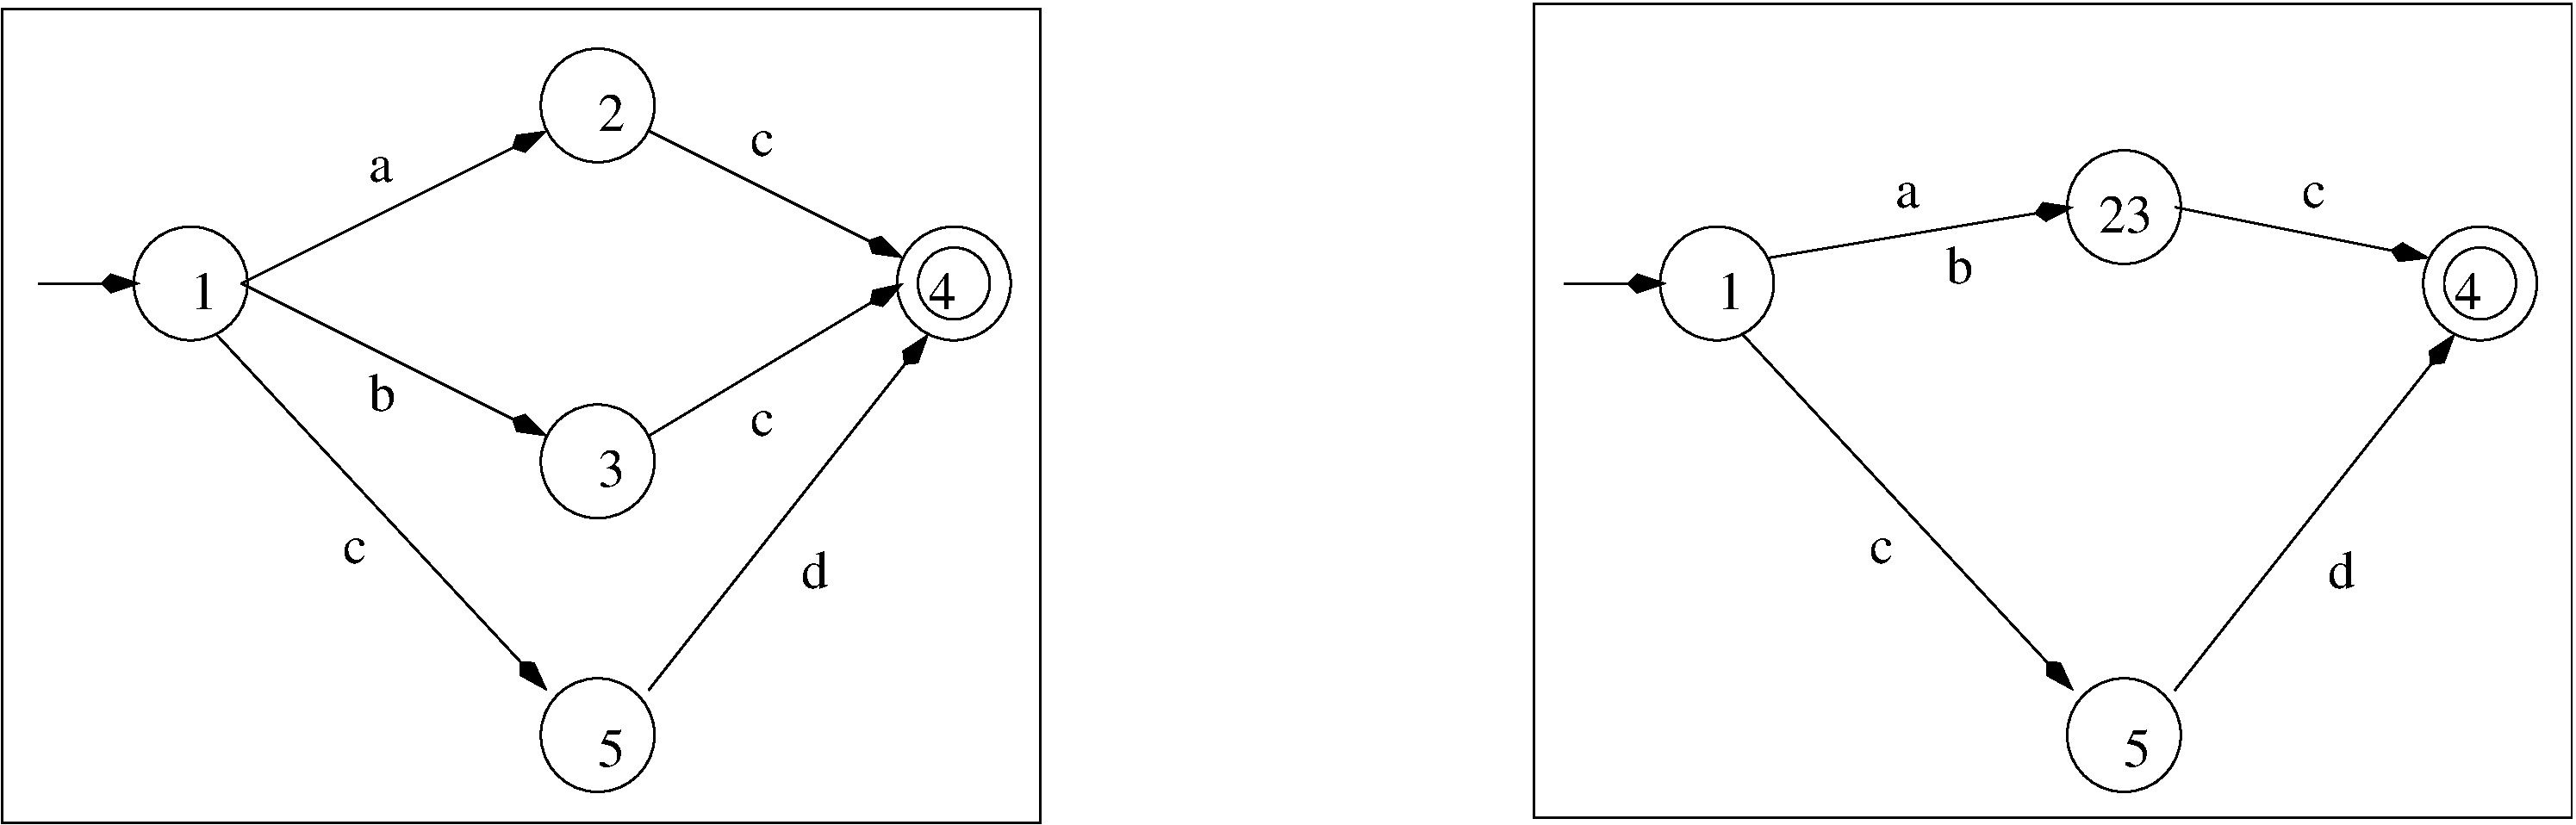
\includegraphics[%
  width=1.0\linewidth,
  keepaspectratio]{mini1}\end{center}
\caption{ Links een DFA met 2 equivalente toestanden; rechts zijn ze
samengenomen\label{mini1}}
\end{figure}


Vanuit de toestanden 2 en 3 vertrekken bogen met hetzelfde label naar
de eindtoestand. Dat geeft aan dat die twee toestanden {\em f-gelijk}
zijn, t.t.z. eens je in 2 of 3 geraakt bent, geraak je met dezelfde
strings tot aan de eindtoestand: de $f$ in f-gelijk staat voor {\em
finaal}. Langs de andere kant: om van 5 naar de eindtoestand te gaan
heb je een andere string nodig dan om van 3 naar de eindtoestand te
gaan, en we noemen 3 en 5 dan ook {\em f-verschillend}.\footnote{In de
literatuur vind je indistinguishable en distinguishable.} De idee van
minimalisatie van een DFA is nu: identificeer verzamelingen van
f-gelijke toestanden en neem die samen.


Voor het gemak zullen we eisen dat vanuit elke toestand er een boog
vertrekt voor elk symbool van het alfabet, m.a.w. dat $\delta$ een
totale functie is; overtuig je ervan dat je hoogstens \'{e}\'{e}n
extra toestand nodig hebt om een DFA die die eigenschap niet heeft
naar een DFA om te vormen met die eigenschap\footnote{Veel auteurs
beschouwen van in het begin enkel DFA's met die eigenschap en relaxen
die later voor het gemak.}.


Laat ons eerst exact defini\"eren wanneer twee toestanden f-verschillend
zijn en wanneer f-gelijk:


\grijs{\begin{definitie}\label{gelijk} f-verschillende en f-gelijke toestanden\\
{\rm Twee toestanden p en q zijn {\bf f-gelijk} indien

$~~~~~~~~~~~~\forall w \in \Sigma^*: \delta^*(p,w) \in F \Longleftrightarrow \delta^*(q,w) \in F$

Twee toestanden zijn {\bf f-verschillend} indien ze niet f-gelijk zijn.
}
\end{definitie}}

Als $p$ en $q$ f-verschillend zijn, dan wil dat zeggen dat er een woord $w$
bestaat zodanig dat

$~~~~~~~~~~\delta^*(p,w) \in F~~en~~ \delta^*(q,w) \notin F$ of omgekeerd.


Nu in woorden een algoritme om sets van f-gelijke toestanden te vinden:
\begin{itemize}
\item[{\bf Init:}]
een toestand $p$ die geen eindtoestand is, is zeker f-verschillend
van elke eindtoestand; alle andere paren toestanden zijn nog onbeslist

\item[{\bf Repeat:}]
neem een paar toestanden $p$ en $q$ dat nog onbeslist is: stel dat er een
symbool $a$ bestaat zodanig dat je met dat symbool van $p$ en $q$ gaat naar
twee f-verschillende toestanden, dan beslis je dat $p$ en $q$ f-verschillend
zijn

\item[{\bf Consolideer:}]
voor elk paar toestanden $p$ en $q$ waarvoor je nog niet beslist had,
beslis nu dat $p$ en $q$ f-gelijk zijn; gebruik die gelijkheidsrelatie
om $Q$ (de toestanden) te partitioneren, t.t.z. te verdelen in
disjuncte $Q_i$ die samen $Q$ uitmaken; de $Q_i$ vormen de toestanden
van de minimale DFA; hoe $\delta$ eruit ziet komt later meer formeel

\end{itemize}


Om wat schrijfwerk uit te sparen zullen we de notatie $p_a$ gebruiken
als afkorting voor $\delta(p,a)$.

\clearpage

\begin{algo} F-gelijke toestanden \label{gelijketoestanden}
\begin{enumerate}
\item[{\bf Init:}]
Beschouw de graaf $V$ met als knopen de toestanden van de DFA; voeg een
boog toe tussen elke twee knopen waarvan er precies \'{e}\'{e}n in F
zit; label die boog met \eps; een boog tussen knopen $x$ en $y$, met
een label $l$, zullen we aanduiden door $(x,y,l)$


\item[{\bf Repeat:}]
\underline{Indien} er knopen $p$ en $q$ zijn waarvoor geldt dat
\begin{itemize}
\item er is geen boog tussen $p$ en $q$
\item $\exists a \in \Sigma: \exists (p_a,q_a,\_) \in V$
\end{itemize}
kies \underline{dan} een $a$ waarvoor geldt dat $(p_a,q_a,\_) \in V$
en voeg de boog $(p,q,a)$ toe aan V; ga terug naar het begin van Repeat;

\underline{anders}: ga naar Gelijk;

\item[{\bf Gelijk:}]
Beschouw de graaf $G$ die als knopen heeft de toestanden uit Q en die
een boog heeft tussen twee knopen $p$ en $q$ indien $V$ {\bf geen} boog
heeft tussen $p$ en $q$ (m.a.w. de complementsgraaf); elke component
van $G$ is een klik (een volledig verbonden graaf, isomorf met $K_n$
voor een n); laat $Q_i$ de verzameling knopen in component $i$
voorstellen; alle toestanden binnen \'{e}\'{e}n $Q_i$ zijn f-gelijk;
elke toestand in $Q_i$ is f-verschillend van elke toestand in $Q_j$
voor $i \neq j$

\end{enumerate}

\end{algo}
\begin{proof}
De eindigheid van het algoritme is evident: in Repeat wordt \'{e}\'{e}n boog
toegevoegd en het maximaal aantal bogen dat $V$ kan hebben is
$N(N-1)/2$ met N het aantal knopen van $V$.


We bewijzen dat


$~~~~~~~~~~~~~~~(p,q,\_)$ is een boog in $V$ $\Longleftrightarrow$ $p$ en $q$ zijn f-verschillend


$\underline{\Longrightarrow}$: indien $(p,q,X)$ een boog is in $V$, dan
zijn er twee mogelijkheden: $X = \epsilon$ of $X = a \in \Sigma$; in het
eerste geval hebben we onmiddellijk dat $p$ en $q$ f-verschillend zijn
(neem daarvoor $w = \epsilon$ in het besluit na de definitie van
f-gelijk op pagina \pageref{gelijk}); in het tweede geval hebben we dat
er een boog bestaat van de vorm $(p_a,q_a,\_)$ in $V$: je ziet nu dat
je het label kunt gebruiken om in het vorige basisgeval terecht te
komen, dus $\exists w \in \Sigma^* : \exists (p_w,q_w,\epsilon) \in
V$, dus $p$ en $q$ zijn f-verschillend.  

$\underline{\Longleftarrow}$: indien $p$ en $q$ f-verschillend zijn, dan
bestaat er een $w$ zodat $\delta^*(p,w) \in F~~en~~\delta^*(q,w) \notin F$
of omgekeerd; als die $w$ de lege string is, dan is het besluit
onmiddellijk; in het andere geval heeft $w$ een laatste symbool $z \in
\Sigma$ en kan geschreven worden als $w = vz$; we hebben dan
$\delta^*(p,w) = \delta(\delta^*(p,v),z)$ dus:
%
tussen de toestanden $\delta^*(p,v)$ en $\delta^*(q,v)$ is er een
boog; we kunnen nu dat laatste symbool van v kwijtgeraken enzovoort
tot we zullen uitkomen op: er is een boog tussen
$\delta^*(p,\epsilon)$ en $\delta^*(q,\epsilon)$ en we zijn klaar.
\end{proof}

\newpage
We hebben nu in de DFA de equivalentieklassen van f-gelijke toestanden
gevonden - de $Q_i$ op het einde van het algoritme - en zijn nu klaar
om de $DFA_{min}$ te defini\"eren: we vertrekken van een DFA
$(Q,\Sigma,\delta,q_s,F)$ zonder onbereikbare toestanden.  

$DFA_{min}$ bestaat uit
$(\tilde{Q},\Sigma,\tilde{\delta},\tilde{q_s},\tilde{F})$
waarbij
\begin{itemize}
\item $\tilde{Q} = \{Q_1, Q_2, ...\}$ waarbij de $Q_i$ verkregen zijn
in het algoritme

\item
$\tilde{\delta}(Q_i,a) = Q_j$ waarbij $Q_j$ verkregen wordt door: neem
een $q \in Q_i$ (*) en neem dan de $Q_j$ zodanig dat $\delta(q,a) \in Q_j$

\item 
$\tilde{q_s}$ is de $Q_i$ waarvoor geldt dat $q_s \in Q_i$

\item
$\tilde{F}$ is de verzameling van $Q_i$ waarvoor geldt dat $Q_i \cap
F \neq \emptyset$
\end{itemize}

Figuur~\ref{minim1} illustreert voor de DFA van Figuur~\ref{mini1} hoe
V evolueert en hoe de complementsgraaf er uitziet.
\begin{figure}[h]
\begin{center}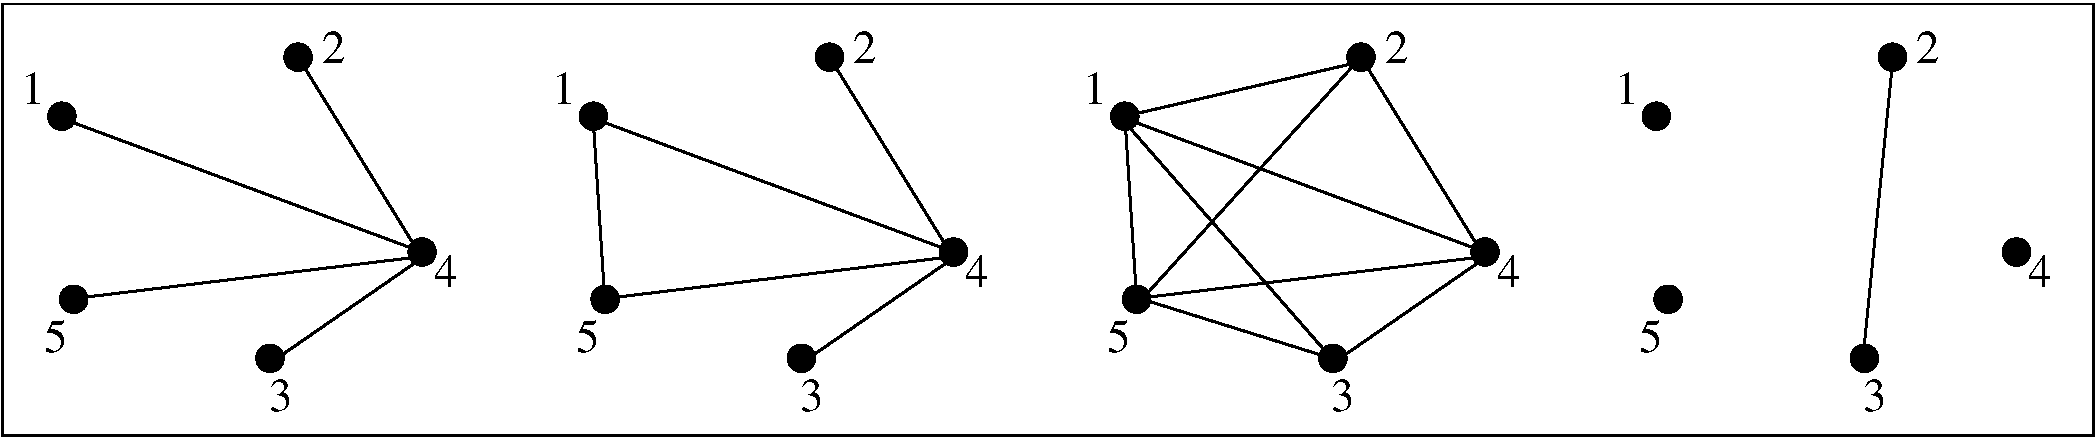
\includegraphics[%
  width=0.9\linewidth,
  keepaspectratio]{minim1}\end{center}
\caption{ 4 tussenstappen in het algoritme\label{minim1}}
\end{figure}
\paragraph{Zelf doen:}
\begin{itemize}
\item[]
In (*) hierboven is het niet belangrijk welke $q \in Q_i$
gekozen wordt: bewijs dat.

Bewijs dat als $Q_i \cap F \neq \emptyset$, dan $Q_i \cap F = Q_i$
(m.a.w. elk element van $Q_i$ zit in F).

Bewijs dat in $DFA_{min}$ elke twee toestanden f-verschillend zijn.

Bewijs tenslotte dat $L_{DFA} = L_{DFA_{min}}$

Wat als je DFA ook onbereikbare toestanden had en je voert die
minimisatieprocedure uit?
\end{itemize}

\project{collapse NFA naar DFA naar DFA(min) in NFA naar DFA(min)}

\newpage
We zouden nu graag bewijzen dat de voorheen geconstrueerde $DFA_{min}$
een minimaal aantal toestanden heeft. We bewijzen een iets algemenere
stelling:

\grijs{\begin{stelling}
Als $DFA_1 = (Q_1,\Sigma,\delta_1,q_s,F_1)$ een machine is zonder
onbereikbare toestanden en waarin elke twee toestanden f-verschillend
zijn, dan bestaat er geen machine met strikt minder toestanden die
dezelfde taal bepaalt.
\end{stelling}
}
\begin{proof}
Laat $DFA_1$ als toestanden hebben $\{q_s,q_1,...,q_n\}$, waarbij
$q_s$ de starttoestand is.  Stel dat
%
$DFA_2 = (Q_2,\Sigma,\delta_2,p_s,F_2)$
minder toestanden heeft dan $DFA_1$.


Vermits in $DFA_1$ elke toestand bereikbaar is, bestaan er strings
$s_i, i=1..n$ zodanig dat
%
$\delta_1^*(q_s,s_i) = q_i$. 


Vermits $DFA_2$ minder toestanden heeft moet voor een $i \neq j$

$~~~~~~~~~\delta_2^*(p_s,s_i) = \delta_2^*(p_s,s_j)$.


Vermits $q_i$ en $q_j$ f-verschillend zijn, bestaat een string $v$ zodanig
dat


$~~~~~~~~~\delta_1^*(q_i,v) \in F_1 \wedge \delta_1^*(q_j,v) \notin F_1$ of
omgekeerd.


Dus ook
%
$\delta_1^*(q_s,s_iv) \in F_1 \wedge \delta_1^*(q_s,s_jv) \notin F_1$ of
omgekeerd. Dit betekent dat $DFA_1$ van de strings $s_iv$ en $s_jv$ er juist \'{e}\'{e}n accepteert.


Maar:
$\delta_2^*(p_s,s_iv) = \delta_2^*(\delta_2^*(p_s,s_i),v) =
\delta_2^*(\delta_2^*(p_s,s_j),v) = \delta_2^*(p_s,s_jv)$
hetgeen betekent
dat $DFA_2$ ofwel beide strings $s_iv$ en $s_jv$ accepteert, of beide
verwerpt.


Dus kunnen $DFA_1$ en $DFA_2$ niet dezelfde taal bepalen.
\end{proof}


De vroeger geconstrueerde $DFA_{min}$ heeft geen onbereikbare
toestanden en elke twee toestanden zijn f-verschillend, dus heeft
$DFA_{min}$ een minimaal aantal toestanden.

% \newpage

Twee DFA's zijn pas echt gelijk als hun toestanden dezelfde zijn, hun
$\delta$ en hun finale toestanden. Maar toch kunnen twee DFA's zo hard
op elkaar gelijken dat hun grafische voorstelling er hetzelfde uitziet
op de naam van de toestanden na. Om dat uit te drukken is er de notie
van isomorfe DFA's.

\grijs{\begin{definitie} Isomorfisme DFA's\\
{\rm
$DFA_1 = (Q_1,\Sigma,\delta_1,q_{s1},F_1)$ is {\bf isomorf} met $DFA_2 =
(Q_2,\Sigma,q_{s2},\delta_2,F_2)$ indien er een bijectie
%
$b: Q_1 \rightarrow Q_2$ bestaat zodanig dat
\begin{itemize}
\item $b(F_1) = F_2$
\item $b(q_{s1}) = q_{s2}$
\item $b(\delta_1(q,a)) = \delta_2(b(q),a)$ (zie Figuur~\ref{diagram1})
\end{itemize}
}
\end{definitie}}
\begin{figure}[h]
\begin{center}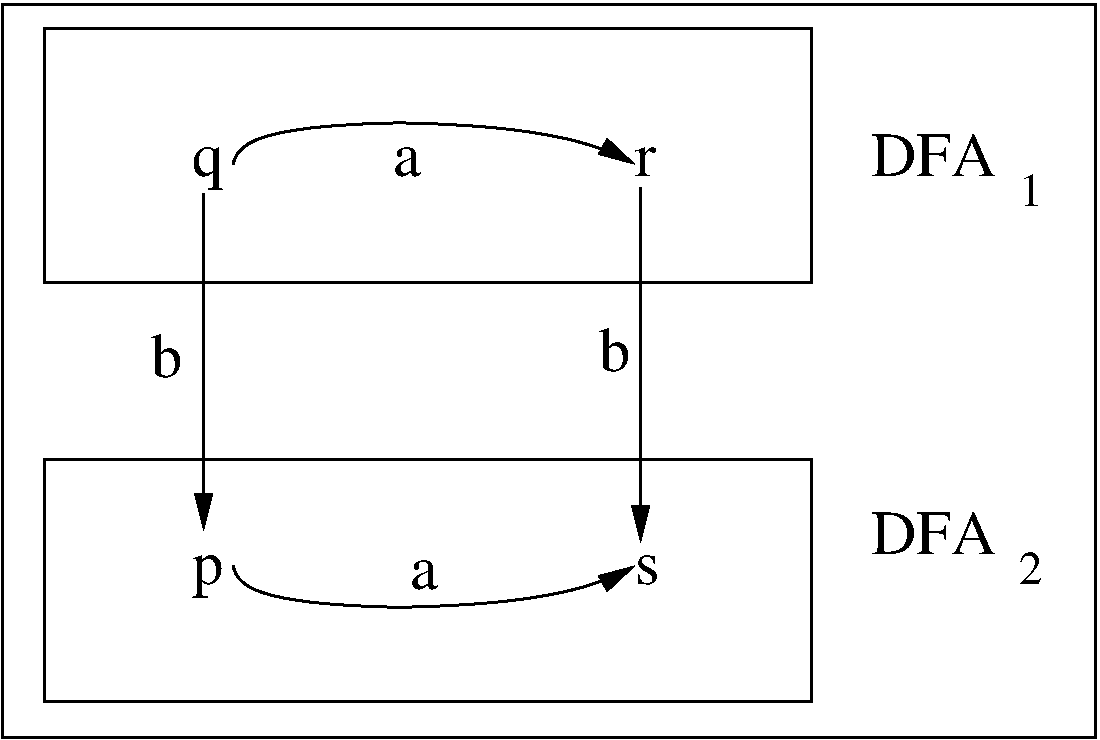
\includegraphics[%
  width=0.4\linewidth,
  keepaspectratio]{diagram1}\end{center}
\caption{Commutatief diagram voor $b$ en $\delta_i$\label{diagram1}}
\end{figure}


Het is gemakkelijk om in te zien dat twee isomorfe DFA's dezelfde taal
bepalen.


We kunnen nu rechtsreeks bewijzen dat de minimale DFA uniek is op
isomorfisme na - probeer het! Maar het kan ook langs een elegante
omweg. De bagage daarvoor krijg je in de volgende sectie.



%% \subsection{De complexiteit van minimizatie en equivalentie}
%% 
%% Een DFA minimalizeren kan in polynoomtijd, maar het minimalizeren
%% van NFA's is NP-hard. Het testen van de equivalentie van reguliere
%% expressies is zelfs PSPACE-hard. Dat kan je intu\"itief argumenteren
%% door te wijzen op het feit dat de conversie van NFA's naar DFA's het
%% aantal toestanden exponentieel kan doen toenemen.

% \clearpage
\section{Het pompen van strings in reguliere talen}

We bekijken hier een manier om van een taal aan te tonen ze niet
regulier is.

Neem een reguliere taal L met oneindig veel strings. Voor L bestaat
een DFA. Die DFA heeft $N = \#Q$ toestanden. Neem een string in L die
langer is dan $N$, en begin met die string in de hand op je tocht van
de starttoestand naar een eindtoestand. Vermits er maar N toestanden
zijn en je string meer dan N lang is en je bij elke overgang juist
\'{e}\'{e}n symbool achterlaat, moet je op je weg naar de eindtoestand
minstens \'{e}\'{e}n toestand S twee keer (of meer) tegenkomen: je
hebt ergens een kring gemaakt. Tijdens die kring heb je een substring
van de oorspronkelijke string gebruikt, t.t.z. je initi\"ele string is
van de vorm $xyz$, waarbij $x$, $y$ en $z$ substrings zijn, $x$ het
stuk voor je aan S kwam, $y$ het stuk van S tot de eerstvolgende weer
aan S, en $z$ alles erna. Probeer je er nu van te overtuigen dat je
die kring twee keer zal doen als je als initi\"ele string $xyyz$ had
gekregen, en dat $xyyz$ ook wordt aanvaard. En hetzelfde voor $xz$, en
$xyyyz$ ... en $xy^iz$ voor elke i.  

Formeel nu:

\grijs{\begin{stelling} Het pompend lemma voor
reguliere talen \\
Voor een reguliere taal L bestaat een pomplengte $d$, zodanig dat als
%
$s \in L$ en $|s| \geq d$, dan bestaat er een verdeling van $s$ in stukken
$x$, $y$ en $z$ zodanig dat $s = xyz$ en
\begin{enumerate}
\item
$\forall i \ge 0: xy^iz \in L$


\item
$|y| > 0$


\item
$|xy| \leq d$
\end{enumerate}


\end{stelling}}

\begin{proof}
Neem een DFA die L bepaalt. Neem $d = \#Q + 1$.

Neem een willekeurige $s = a_1a_2...a_n$ met $n \geq d$.
Beschouw de accepterende sequentie van toestanden
$(q_s=q_1,q_2,...,q_f)$ voor s; die heeft lengte strikt groter dan
$d$, dus zijn er bij de eerste $d$ zeker twee toestanden gelijk
(omdat er maar $d-1$ toestanden zijn).  Stel dat $q_i$ en $q_j$ gelijk
zijn met $i < j \leq d$ dan nemen we $x = a_1a_2...a_{i}$ en $y =
a_{i+1}...a_j$ en $z$ de rest van de string. Alles volgt nu
direct.  Figuur~\ref{pomp1} illustreert de verdeling van $s$ in $xyz$.\end{proof}

\begin{figure}[h]
\begin{center}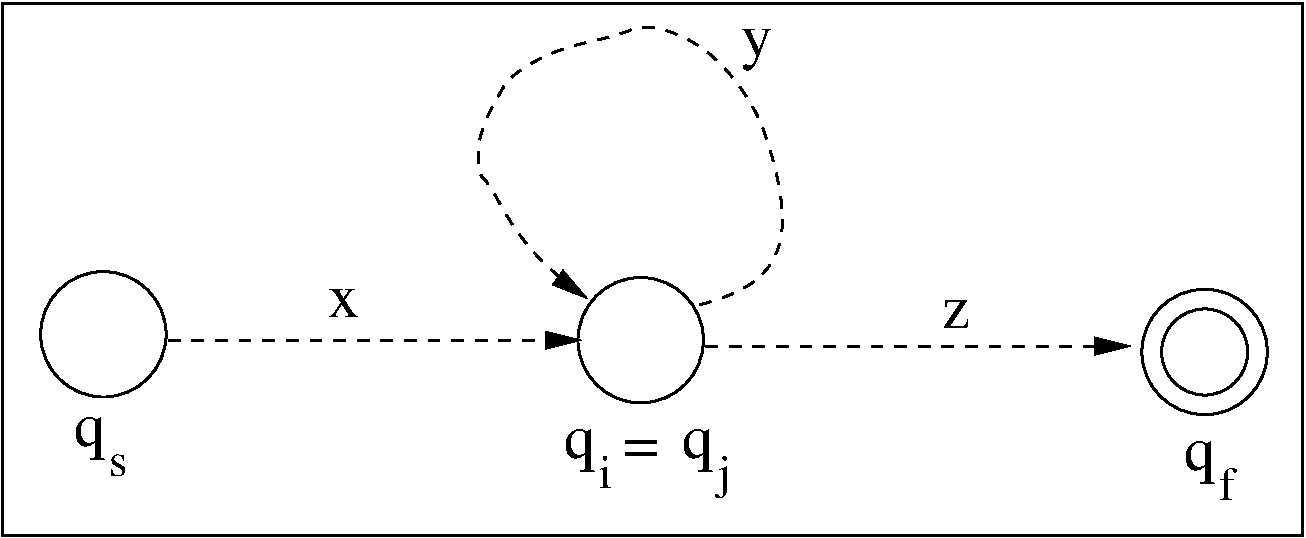
\includegraphics[%
  width=0.5\linewidth,
  keepaspectratio]{pomp1}\end{center}
\caption{Illustratie van de verdeling van de string \label{pomp1}}
\end{figure}


\subsection{Het pompend lemma gebruiken}

Het is belangrijk eerst voor
jezelf uit te maken dat het pompend lemma niet nuttig is om te
bewijzen dat een taal regulier is - probeer maar :-)


We kunnen het wel gebruiken om te bewijzen dat een gegeven taal niet
regulier is. Als voorbeeld nemen we nog eens de taal $L = \{a^nb^n|n
\in \N\}$ over het alfabet $\{a,b\}$.  


Stel dat er voor die taal een pomplengte $d$ bestond, beschouw dan de
string $s = a^db^d$. Neem een willekeurige opdeling van $s = xyz$ met
$|y| > 0$. Dan zijn er drie mogelijkheden

\begin{itemize}
\item y bevat alleen a's: dan bevat xyyz meer a's dan b's en zit dus niet in L
\item y is van de vorm $a^ib^j$ met $i \neq 0, j \neq 0$: dan bevat
xyyz niet alle a's voor de b's, en zit dus niet in L
\item y bevat alleen b's: dan bevat xz meer a's dan b's en zit dus niet in L
\end{itemize}

Bijgevolg kan L niet regulier zijn.


We hebben punt 3 van het lemma niet gebruikt. Als je dat wel wil doen,
dan gaat het bewijs dat L niet regulier is soms korter of
gemakkelijker. In dit geval wordt het:


Stel dat er voor die taal een pomplengte $d$ bestond, beschouw dan de
string $s = a^db^d$. Neem een willekeurige opdeling van $s = xyz$ met
$|y| > 0$ en $|xy| \leq d$. Dan bestaat $y$ uitsluitend uit a's en dus
bevat xz minder a's dan b's en zit dus niet in L.



\paragraph{Merk op:} Het pompend lemma gebruiken om te
bewijzen dat L niet in RegLan zit, heeft de volgende ingredi\"enten:
\begin{itemize}
\item voor een willekeurig getal d gekozen als pomplengte
\item bestaat een string s langer dan d
\item waarvoor {\bf elke} opdeling pompen verhindert
\end{itemize}

Vooral dat laatste realiseren is belangrijk - hier een voorbeeld:
neem L de taal gegenereerd door de reguliere expressie $ab^*c$.
We gaan (verkeerdelijk) bewijzen dat L niet regulier is door (foutief)
gebruik te maken van het pompend lemma. Neem een willekeurige
pomplengte d (groter dan bijvoorbeeld 10), en neem een willekeurige
string met lengte groter dan d+1. De string is van de vorm $ab^ic$ met
$i > 9$. Neem voor x,y en z uit de stelling $x = \epsilon$, $y = a$ en
$z = b^ic$. Het is nu duidelijk dat xyyz niet behoort tot L en dus
kunnen we de string niet pompen. Dus is L niet regulier ...

\paragraph{Zelf doen:}
\begin{itemize}
\item[]
Welke fout werd hierboven gemaakt?

Definieer wat talen en gebruik het pompend lemma om na te gaan of ze
regulier (kunnen) zijn. Is de taal van reguliere expressies regulier?

Bestaat een niet-reguliere taal waarvan elke string kan gepompt worden?
%% welke was dat weer? a^nb^mc^i als n = 1, dan m=i

Bestaat er een minimale pomplengte voor elke taal? Is er een verband
met de minimale DFA voor die taal?
\end{itemize}

\clearpage

\section{Doorsnede, verschil en complement van DFA's}

We hebben al wel de unie van reguliere talen bekeken, maar nog niet de
andere gebruikelijke set-operaties: doorsnede, (symmetrisch) verschil
en complement. Stel gegeven twee DFA's
$(Q_i,\Sigma,\delta_i,q_{si},F_i)$ voor i=1,2. We maken een
generische product DFA $(Q,\Sigma,\delta,q_s,F)$ als volgt:

\begin{itemize}
\item $Q = Q_1 \times Q_2$
\item $\delta(p \times q,x) = \delta_1(p,x) \times \delta_2(q,x)$
\item $q_s = q_{s1} \times q_{s2}$
\end{itemize}

Nu moeten we enkel nog $F$ bepalen om te komen tot een volledige
definitie. Dat kan natuurlijk op verschillende manieren. Hier zijn er
een aantal:

\begin{itemize}
\item $F = F_1 \times F_2$: de DFA is nu de doorsnede van de twee talen
\item $F = (F_1 \times Q_2) \cup (Q_1 \times F_2)$: de DFA is nu de unie
van de twee talen
\item $F = F_1 \times (Q_2 \setminus F_2)$: de DFA bepaalt nu de strings die
tot $L_1$ behoren, maar niet tot $L_2$
\item $F = (Q_1 \setminus F_1) \times (Q_2 \setminus F_2)$: de DFA bepaalt nu de
strings die tot geen van beide talen behoren
\end{itemize}

De bovenstaande constructies tonen aan dat de unie (dat wisten we al),
de doorsnede, het verschil en het symmetrisch verschil van twee
reguliere talen ook regulier is. Daaruit volgt ook dat het complement
van een reguliere taal regulier is, want
%
$\overline{L} = \Sigma^* \setminus L$.

\paragraph{Zelf doen:}
\begin{itemize}
\item[]
Vind een eenvoudigere constructie van een complements-DFA als de DFA
van een taal gegeven is.

Als diezelfde constructie wordt gedaan op een NFA, krijg je dan nog
wat je bedoelde? Waarom (niet)?
\end{itemize}






\clearpage
\section{Reguliere expressies en lexicale analyse}


Met een reguliere expressie kan dikwijls gemakkelijk gespecifieerd
worden welke {\em input} in een bepaalde context toegelaten
is. Bijvoorbeeld: 


~~~~~~~~~~~~$20(0|1|2|3|4|5|6|7|8|9)(0|1|2|3|4|5|6|7|8|9)$


geeft aan dat ergens alleen een jaartal in deze eeuw mag
ingetypt worden. 


Voor programmeertalen wordt heel dikwijls van RE's gebruik gemaakt om
het lexicon van de taal te defini\"eren. Een klein stukje van het
lexicon van Java zou kunnen zijn:
$(a|b|c)(a|b|c|0|1|2)^*~|~(-|\epsilon)(1|2)(0|1|2)^*$ waarmee we dan identifiers
kunnen beschrijven die met \'{e}\'{e}n van de letters a,b of c
beginnen en dan nog een willekeurig aantal letters en cijfers (enkel
0,1,2) kunnen bevatten, en gehele getallen die optioneel een minteken
hebben en dan ...


Het wordt snel omslachtig als we geen afkortingen gebruiken en het is
dus gebruikelijk om zulke specificatie van het lexicon te doen als volgt:


~~~~~~~~~~~~$PosCijfer \leftarrow 1~|~2~|~3~|~4~|~5~|~6~|~7~|~8~|~9$

~~~~~~~~~~~~$Cijfer \leftarrow PosCijfer~|~0$


en dan kan dat jaartal voorgesteld worden als 


~~~~~~~~~~~~$DezeEeuw \leftarrow 20CijferCijfer$


en de algemene vorm van een integer als $(+|-|\epsilon)PosCijfer~Cijfer^*~|~0$


en voor een veld waarin een bankrekeningnummer moet ingetypt worden:


~~~~~~~~~~~~$BANKNR \leftarrow Cijfer^3(-~|~\epsilon)Cijfer^7(-~|~\epsilon)Cijfer^2$


Op die manier wordt het nu eenvoudig om een beschrijving te geven van
het lexicon van bijvoorbeeld een programmeertaal. Hier is een stukje
uit de beschrijving van Java:

% \clearpage

\begin{itemize}
\item[]
$JavaProgr \leftarrow (Id|Int|Float|Op|Delimiter)^*$

$Id \leftarrow Letter~(Letter|Cijfer)^*$

$Cijfer \leftarrow PosCijfer~|~0$

$PosCijfer \leftarrow 1~|~2~|~3~|~4~|~5~|~6~|~7~|~8~|~9$

$Teken \leftarrow (+|-|\epsilon)$

$Unsigned \leftarrow PosCijfer~Cijfer^*$

$Int \leftarrow Teken~Unsigned$

$Float \leftarrow Int~.~Unsigned$

...
\end{itemize}

\label{flexlabel}Die beschrijving kan gebruikt worden om een lexer te
maken voor Java, t.t.z. een programma dat aan lexicale analyse van een
reeks tekens doet en beslist of ze behoren tot de taal (Java in dit
geval). Er bestaan natuurlijk tools om gegeven een beschrijving
van een lexicon m.b.v. reguliere expressies en afkortingen zoals
hierboven, de benodigde automaten te genereren en de juiste glue-code
om het zaakje werkende te houden. Zo vind je flex (zie
\verb|http://flex.sourceforge.net/|) dat C-code genereert: die C-code
implementeert de DFA's en de glue-code. jflex
(\verb|http://www.jflex.de/|) is op hetzelfde principe gebaseerd en
genereert Java-code. flex en jflex zijn lexicale analyse generatoren.

\paragraph{Zelf doen:}
\begin{itemize}
\item[]
Lees meer over (j)flex.

Probeer vanuit een reguliere expressie E een Prolog programma te
genereren, met een predicaat lex/1 dat opgeroepen met een string s
slaagt alss s tot $L_E$ behoort: een string zoals abc stel je in
Prolog voor door $[a,b,c]$. Een RE zoals $a^*b~|~c$ kan je voorstellen
als de term $of([ster(a),b],[c])$ (maar kan ook anders).
\end{itemize}

\paragraph{De beschrijving} van bijvoorbeeld $JavaProgr$ hierboven, is
een BNF-grammatica, anders gezegd {\em staat in Backus-Nauer vorm}:
eigenlijk is die bedoeld voor context-vrije talen. BNF kan je ook
gebruiken voor reguliere talen, omdat die ook context-vrij zijn: zie
Sectie~\ref{contextvrijetalen}.

\newpage 
\section{Varianten van eindige toestandsautomaten}

\subsection{Transducer}

\project{minimisatie van transducer}

Een transducer zet een string om in een andere: we passen de definitie
van een DFA een beetje aan, zodat ook output kan geproduceerd worden.
E\'{e}n figuur is bijna een definitie waard:

\begin{figure}[h]
\begin{center}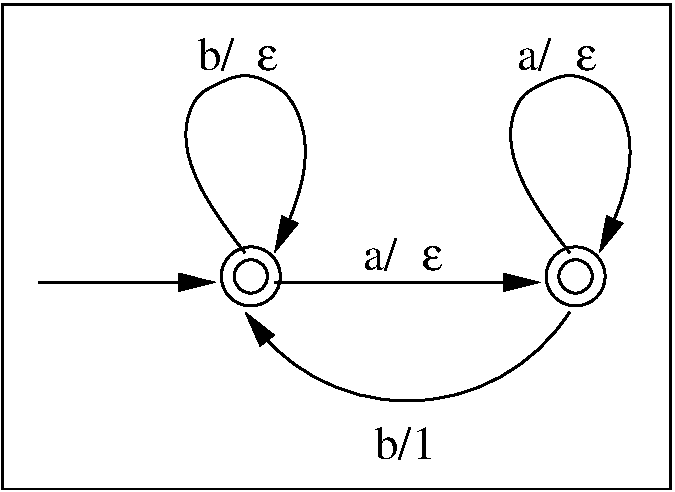
\includegraphics[%
  width=0.35\linewidth,
  keepaspectratio]{trans1}\end{center}
\caption{Een eenvoudige transducer \label{trans1}}
\end{figure}

De labels zijn nu van de vorm $a/x$ waarbij a in het inputalfabet zit
en x in een outputalfabet (inbegrepen de lege string). Wat voor de /
staat wordt gebruikt om de weg te vinden in de transducer alsof het
een DFA was. Wat na de / staat wordt op de output gezet als die boog
genomen wordt. Bovenstaande transducer accepteert elke string en
geeft als output een 1 voor elke b die vlak na een a komt.



\subsection{Een optelchecker m.b.v. een DFA}

Een DFA kan alleen gebruikt worden om te beslissen of een string
behoort tot een taal. Zo zou je kunnen een taal defini\"eren van strings
die correcte optellingen voorstellen en als die taal regulier is er
een DFA voor bouwen. Hier is een poging: $\Sigma = \{0,1\}$ . De twee
getallen die we willen optellen en het resultaat komen in binair,
omgekeerd en we maken ze even lang door bij de kortste(n) wat leidende
nullen toe te voegen. Dus als we 3 willen optellen bij 13, met
resultaat 16, dan hebben we de drie bitstrings 11000 10110 en
00001. Die mengen we nu systematisch, t.t.z. we maken groepjes van 3
bits die op de i-de plaats voorkomen en schrijven die groepjes achter
elkaar. Dus we hebben

$~~~~~~~~~~~~~~$110 100 010 010 001

waarbij de blanco's enkel dienen om de groepering per drie te laten
zien. Dus de string 110100010010001 stelt de correcte optelling 
3+13=16 voor. Een DFA voor de taal van correcte optellingen staat in
Figuur~\ref{telop}.


\begin{figure}[h]
\begin{center}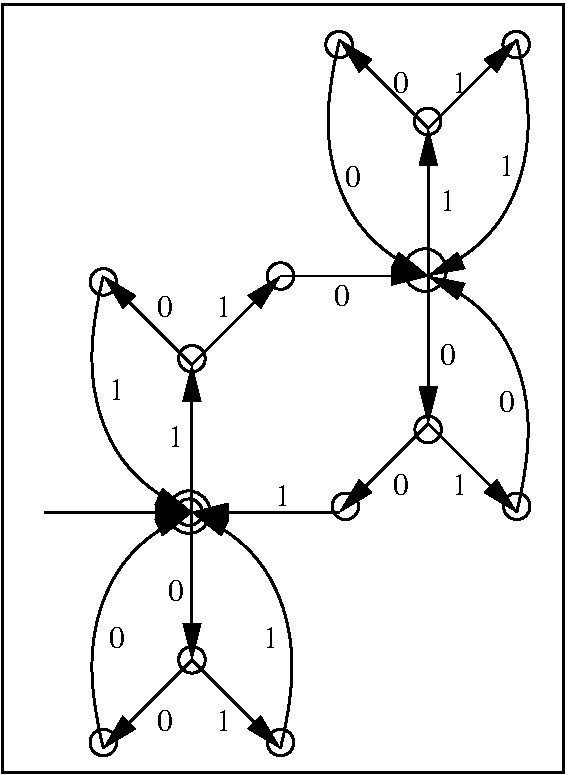
\includegraphics[%
  width=0.25\linewidth,
  keepaspectratio]{telop}\end{center}
\caption{Een optelchecker \label{telop}}
\end{figure}

\newpage
\subsection{Een opteller m.b.v. een transducer}

Optellen bestaat eigenlijk in: gegeven twee getallen als input, output
de som. Dat kan met een transducer: gebruik dezelfde voorstelling van
de twee getallen die je wil optellen als hiervoor, en meng die op
dezelfde manier, dus 3+13 wordt voorgesteld als de string
1110010100. Figuur~\ref{telop2} toont twee optel-transducers die van de
optelchecker zijn afgeleid.

\begin{figure}[h]
\begin{center}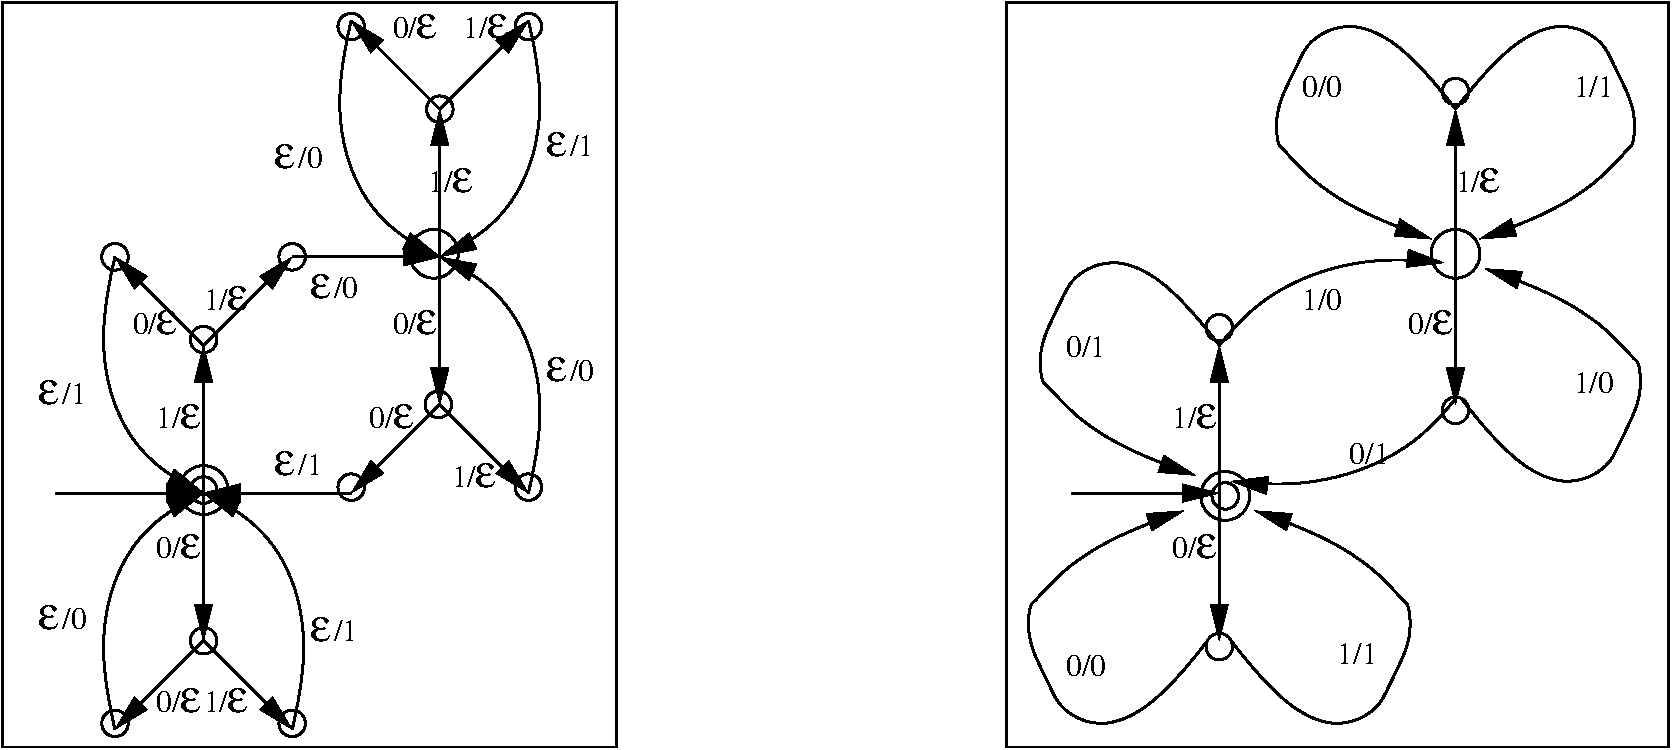
\includegraphics[%
  width=0.7\linewidth,
  keepaspectratio]{telop2}\end{center}
\caption{Twee transducers die als output de som geven \label{telop2}}
\end{figure}

\newpage
\paragraph{Zelf doen:}
\begin{itemize}
\item[]
Kan je met een transducer ook andere rekenkundige bewerkingen doen,
bijvoorbeeld min of maal?

Is de output van een transducer ook een reguliere taal?

Kan je een transducer schrijven die elk derde teken uit een
inputstring geeft?

Kan je een transducer schrijven die elk derde teken uit een
inputstring niet geeft?

Kan je een transducer schrijven die inputstrings omgekeerd uitschrijft?

Kan je elke reguliere taal als output van een transducer krijgen?
\end{itemize}

\subsection{Two-way finite automata}

Een DFA wordt ook wel een {\em one-way finite automaton} genoemd. De
reden is dat je hem ook kan beschrijven als een machine met een
invoerband waarop de inputstring staat. Die machine heeft een leeskop
die in de begintoestand op het eerste teken staat, en bij elke
overgang \'{e}\'{e}n positie naar rechts opschuift in de input: altijd in
dezelfde richting, namelijk naar het einde van de string toe.


Het is slechts een kleine aanpassing aan de automaat om toe te laten
dat de leeskop in twee richtingen mag bewegen: daarvoor pas je de
definitie van $\delta$ gepast aan (zie in hoofdstuk
\ref{berekenbaarheid} hoe dat voor de Turingmachines gebeurt). 
Je krijgt dan een 2DFA.


Van andere klassen van automaten is het geweten dat meer vrijheid
laten in de manipulatie van het {\em geheugen} aanleiding geeft tot
meer berekeningskracht: om dit te appreci\"eren moeten we daarmee eerst
nog kennismaken natuurlijk, maar denk eraan bij de PDA en de LBA.


De vraag {\em is een 2DFA krachtiger dan een DFA}, of {\em zijn er
niet-reguliere talen die met een 2DFA kunnen herkend worden} is dus
van belang. Het blijkt dat de 2DFA ook enkel de reguliere talen
bepaalt.

\project{hier kan zeker een mooi ding mee gedaan worden}

\clearpage
\subsection{B\"{u}chi automaten}

B\"{u}chi\footnote{Julius B\"{u}chi} automaten trekken op NFA's maar
je geeft er geen eindige strings aan, wel oneindig lange: er is dus
geen moment waarop je string {\em op} is bij het doorlopen van de
automaat en de definitie van welke strings geaccepteerd worden door de
B\"{u}chi automaat moet worden aangepast. Die definitie wordt:

\grijs{\begin{definitie}
{\rm
Een oneindige string $s$ wordt aanvaard door een B\"{u}chi automaat
indien de rij toestanden waarlangs je passeert oneindig dikwijls
een aanvaardende toestand heeft.
}
\end{definitie}}

Je kan dat natuurlijk niet uitproberen, maar daarvoor dienen B\"{u}chi
automaten niet noodzakelijk: je modelleert er een probleem mee
(bijvoorbeeld een oneindig repetitief process, een protocol ...) en
bewijst dan voor welke strings de acceptance conditie waar is.  

Niet-deterministische B\"{u}chi automaten zijn strikt sterker dan
deterministische B\"{u}chi automaten: als voorbeeld kan je voor
taal $(a|b)^*b^\omega$ eens een B\"{u}chi automaat proberen te maken.

\project{buchi automaten bestuderen ?}


\clearpage
\section{Referenties}

\setlength{\intextsep}{0pt}
\begin{wrapfigure}[7]{r}{0.19\textwidth}
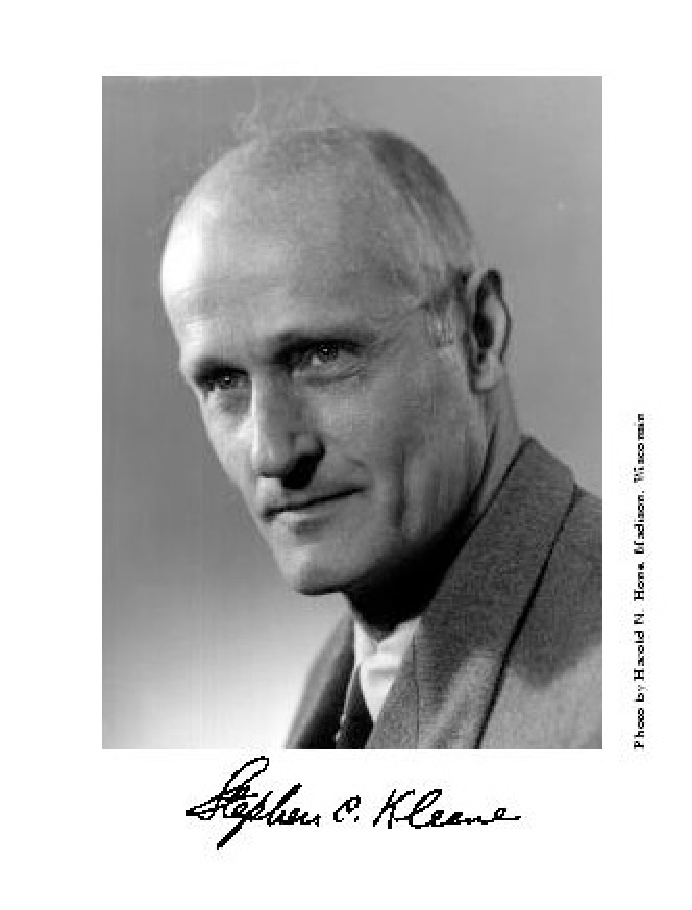
\includegraphics[width=.19\textwidth,keepaspectratio]{afbeeldingen/kleene}
\end{wrapfigure}

Veel van wat je hierboven leerde is afkomstig van Stephen Kleene,
die je ook al kende van een fixpoint stelling. Hij heeft ook bijdragen
geleverd in logica, recursie theorie en intu\"{i}tionisme.


In moderne teksten over reguliere talen/expressies/machines is de
volgorde niet altijd dezelfde, maar de vorige hoofdstukken hebben
aangetoond dat het kip\&ei probleem niet bestaat: ze zijn equivalent.
Ook zijn er dikwijls kleine verschillen in de basisdefinities, maar
ook die maken niks uit: bijvoorbeeld of $\delta$ totaal is of niet, of
er meer dan \'{e}\'{e}n eindtoestand is ... 


Eenzelfde diversiteit in aanpak/definities vinden we later ook terug
bij andere talen/machines en we proberen oog te hebben voor die
verschillen, maar de equivalenties ervan in te zien.




\paragraph{Referenties:}

\begin{itemize}
\item 
Dexter C. Kozen  {\em Automata and Computability} 

\item 
Peter Linz {\em An Introduction to Formal Languages and Automata}

\item 
Michael Sipser {\em Introduction to the Theory of Computation}

\item
John E. Hopcroft, Rajeev Motwani, Jeffrey D. Ullman
{\em Introduction to Automata Theory, Languages, and Computation}

\item
Marvin Lee Minsky {\em Computation: Finite and Infinite Machines
(Automatic Computation)}
\end{itemize}


Als je hierdoor begeesterd wordt, vergeet dan ook niet een andere
standaard referentie: {\em Regular algebra and finite
machines}\footnote{Dit werk staat niet in onze bib, maar als je
ge\"{i}nteresseerd bent, kom eens langs.} van John Horton Conway -
dezelfde die {\em The Game of Life} uitvond dat later in deze tekst
nog aan bod komt, en nog zoveel andere boeiende zaken (o.a. het {\em
Angels and Devils game}) die aan ons inzicht in algoritmiek
rechtsreeks aanbelangen.

\clearpage

\paragraph{Zelf doen:}

Als L1 en L2 reguliere talen zijn, is L3 dan ook regulier?
We spreken af dat het alfabet altijd hetzelfde is en minstens a en b
bevat. We gebruiken de notatie $\hat{s}$ om de string aan te duiden
die dezelfde tekens als $s$ bevat maar in omgekeerde volgorde. Schrijf
telkens formeel neer wat L3 is.
\begin{itemize}
\item[]
L3 is strings van gelijke lengte uit L1 en L2 gemengd (schrijf formeel neer wat gemengd is)

L3 = $\widehat{L1}$

L3 is strings van even lengte uit L1

L3 is strings s van even lengte uit L1 en die dan in twee gekapt s1s2
met gelijke lengte en dan s1 concat omgekeerde van s2

L3 is strings s van L1 en dan s concat omgekeerde van s

L3 is strings van L1 met elke a vervangen door b

L3 is alles uit L1 dat niet in L2 zit

L3 is de taal van strings uit L1 waarin de symbolen op de even
plaatsen weggenomen zijn

$L3 = \{x|\exists y \in L2, xy \in L1\}$

$L3 = \{x|\exists y \in L2, yx \in L1\}$

\end{itemize}


\clearpage

\section{Contextvrije talen en hun grammatica}\label{contextvrijetalen}

Reguliere expressies geven een manier om een taal te bepalen. Een
kleine uitbreiding aan RE's is het toelaten van {\em afkortingen} voor
RE's om op die manier kortere beschrijvingen van een taal te
verkrijgen. Een afkorting bestaat erin van een naam te geven aan een
ding en als je op een bepaalde plaats de naam gebruikt hebt, mag je
daar het ding zelf zetten (of een kopie ervan) en dan is de betekenis
nog dezelfde en de naam is weg. Maar bijvoorbeeld in


~~~~~~~~~Haakjes \rpijl HaakjesHaakjes $|$ [Haakjes] $|$ $\epsilon$


kan je het symbool Haakjes niet kwijtgeraken door substitutie. Toch
kunnen we die regel gebruiken om een taal te genereren. Zulke regels
vormen een {\em contextvrije grammatica}. Voor we een definitie
geven, eerst nog wat voorbeelden:

\begin{vb}
~~~
\begin{itemize}
\item
S \rpijl aSb

S \rpijl \eps

Deze grammatica beschrijft strings van de vorm $a^nb^n$

\item 

S \rpijl PQ

P \rpijl aPb

P \rpijl \eps

Q \rpijl cQd

Q \rpijl \eps

Deze grammatica beschrijft strings van de vorm $a^nb^nc^md^m$


\item \label{statlabel}
Stat \rpijl Assign

Stat \rpijl ITE

ITE \rpijl If Cond Then Stat Else Stat

ITE \rpijl If Cond Then Stat 

Cond \rpijl Id == Id

Assign \rpijl Id := Id

Id \rpijl a

Id \rpijl b

Id \rpijl c

\end{itemize}

\end{vb}

Informeel kunnen we zeggen: een contextvrije grammatica (CFG) bestaat
uit regels; aan de linkerkant van een regel staat een
niet-eindsymbool; aan de rechterkant staat een opeenvolging van
eindsymbolen, niet-eindsymbolen en \eps. Er is een startsymbool.  

Je kan een CFG gebruiken om strings te genereren, en om na te gaan of
een string voldoet aan de grammatica. Genereren doe je door een
afleiding te maken vertrekkend van het startsymbool. Voor het eerste
voorbeeld is wat volgt een afleiding:

$~~~~~~~~~~S$ \rpijl $aSb$ \rpijl $aaSbb$ \rpijl $aabb$


De idee achter afleiding is: in een string waarin nog een
niet-eindsymbool staat, kies een niet-eindsymbool X en vervang X door
de rechterkant van een regel waarin X links voorkomt. Begin met het
startsymbool en werk door tot er alleen nog eindsymbolen staan.


We kunnen die afleiding ook voorstellen in een {\em syntax boom} of
{\em parse tree}: zie Figuur~\ref{parsetree1}.

\medskip
\begin{figure}[h]
\begin{center}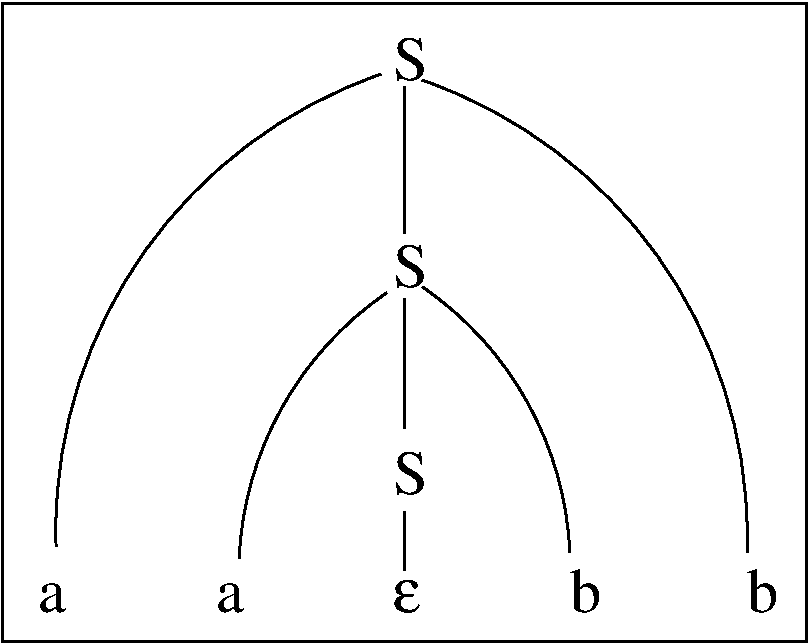
\includegraphics[%
  width=0.4\linewidth,
  keepaspectratio]{parsetree1}\end{center}
\caption{Syntaxboom van aabb \label{parsetree1}}
\end{figure}


\grijs{\begin{definitie} Contextvrije grammatica - CFG\\
{\rm
Een contextvrije grammatica is een 4-tal $(V,\Sigma,R,S)$ waarbij
\begin{itemize}
\item 
$V$ een eindige verzameling niet-eindsymbolen is (ook variabelen
genoemd, of non-terminals)
\item 
$\Sigma$ een eindig alfabet van eindsymbolen (terminals), disjunct
met V
\item 
$R$ is een eindige verzameling regels (of producties); een regel is
een koppel van \'{e}\'{e}n niet-eindsymbool en een string van
elementen uit
$V \cup \Sigma_\epsilon$;
\\
we schrijven de twee delen van zulk een koppel met een \rpijl ertussen
\item 
$S$ is het startsymbool en behoort tot $V$
\end{itemize}

}
\end{definitie}}
Dikwijls ligt het voor de hand welke de eindsymbolen zijn en welk
symbool het startsymbool is: we geven dan alleen de regels.

\grijs{\begin{definitie} Afleiding m.b.v. een CFG\\
{\rm
Gegeven een CFG $(V,\Sigma,R,S)$.
Een string $f$ over $V \cup \Sigma_\epsilon$ wordt afgeleid uit een
string $b$ over $V \cup \Sigma_\epsilon$ m.b.v. de CFG als er een
eindige rij strings $s_0, s_1, ..., s_n$ bestaat zodanig dat
\begin{itemize}
\item $s_0 = b$
\item $s_n = f$
\item $s_{i+1}$ verkregen wordt uit $s_i$ (voor $i < n$) door in $s_i$
een niet-eindsymbool $X$ te vervangen door de rechterkant van een
regel waarin $X$ links voorkomt.
\end{itemize}

We noteren: $s_i \Rightarrow s_{i+1}$ en $b \Rightarrow^* f$
}
\end{definitie}}

\grijs{\begin{definitie} Taal bepaald door een CFG\\
{\rm
De taal $L_{CFG}$ bepaald door een CFG $(V,\Sigma,R,S)$ is de
verzameling strings over $\Sigma$ die kunnen afgeleid worden van het
startsymbool $S$; formeel: $L_{CFG} = \{s \in \Sigma^* | S
\Rightarrow^* s\}$.

}
\end{definitie}}

\grijs{\begin{definitie} Contextvrije taal - CFL\\
{\rm
Een taal $L$ is {\bf contextvrij} indien er een CFG bestaat zodanig
dat $L = L_{CFG}$
}
\end{definitie}}

We zullen i.v.m. contextvrije talen zowat dezelfde weg bewandelen als
voor reguliere talen: we defini\"eren een machine die contextvrije
talen bepaalt en we bewijzen dat die machines {\em equivalent} zijn
met de contextvrije grammatica's; we bestuderen het verschil tussen
deterministische en niet-deterministische versies van die machines; we
maken een versie van het pompend lemma voor contextvrije talen; we
bestuderen de algebra\"{i}sche operaties op de contextvrije talen. We
zullen niet aan minimizatie doen. We zullen aandacht besteden aan
ambigu\"{i}teit: dit probleem hebben we niet bij reguliere talen besproken
omdat het daar niet belangrijk is.  

\subsection{Ambigu\"{i}teit}

We nemen als voorbeeld de CFG Arit1\label{arit1label}
\begin{itemize}
\item Expr \rpijl Expr + Expr
\item Expr \rpijl Expr * Expr
\item Expr \rpijl a
\end{itemize}
waarbij Expr het startsymbool is. Neem de string $a+a*a$: die zit
duidelijk in de taal bepaald door de Arit1. Bekijk nu de twee
afleidingen van die string (we onderlijnen de gesubstitueerde
non-terminal als er keuze is): 

~~~~~$Expr \Rightarrow \underline{Expr} + Expr \Rightarrow a + Expr \Rightarrow a + \underline{Expr} * Expr$

$~~~~~~~~~~\Rightarrow a + a * Expr \Rightarrow a + a * a$

en

~~~~~$Expr \Rightarrow Expr + \underline{Expr} \Rightarrow Expr + Expr * \underline{Expr} \Rightarrow Expr + \underline{Expr} * a$

$~~~~~~~~~~\Rightarrow Expr + a * a \Rightarrow a + a * a$


In de eerste afleiding hebben we telkens het meest linkse
niet-eindsymbool verder ontwikkeld, en in de tweede afleiding het
meest rechtse. Maar als we die afleidingen omzetten naar een parse
tree krijgen we twee keer hetzelfde. Die afleidingen zijn dus niet
essentieel verschillend en dikwijls zullen we daarom ook enkel kijken
naar meest-linkse\footnote{In het engels: leftmost derivation.}
afleidingen.


Beschouw nu de volgende twee meest-linkse afleidingen van $a+a*a$:



~~~~~$Expr \Rightarrow Expr + Expr \Rightarrow a + Expr \Rightarrow a + Expr * Expr$

$~~~~~~~~~~\Rightarrow^* a + a * a$

en

~~~~~$Expr \Rightarrow Expr * Expr \Rightarrow Expr + Expr * Expr  \Rightarrow a + Expr * Expr$

$~~~~~~~~~~\Rightarrow^* a + a * a$

of in termen van de overeenkomstige parse trees: zie Figuur~\ref{ambi1}:

\begin{figure}[h]
\begin{center}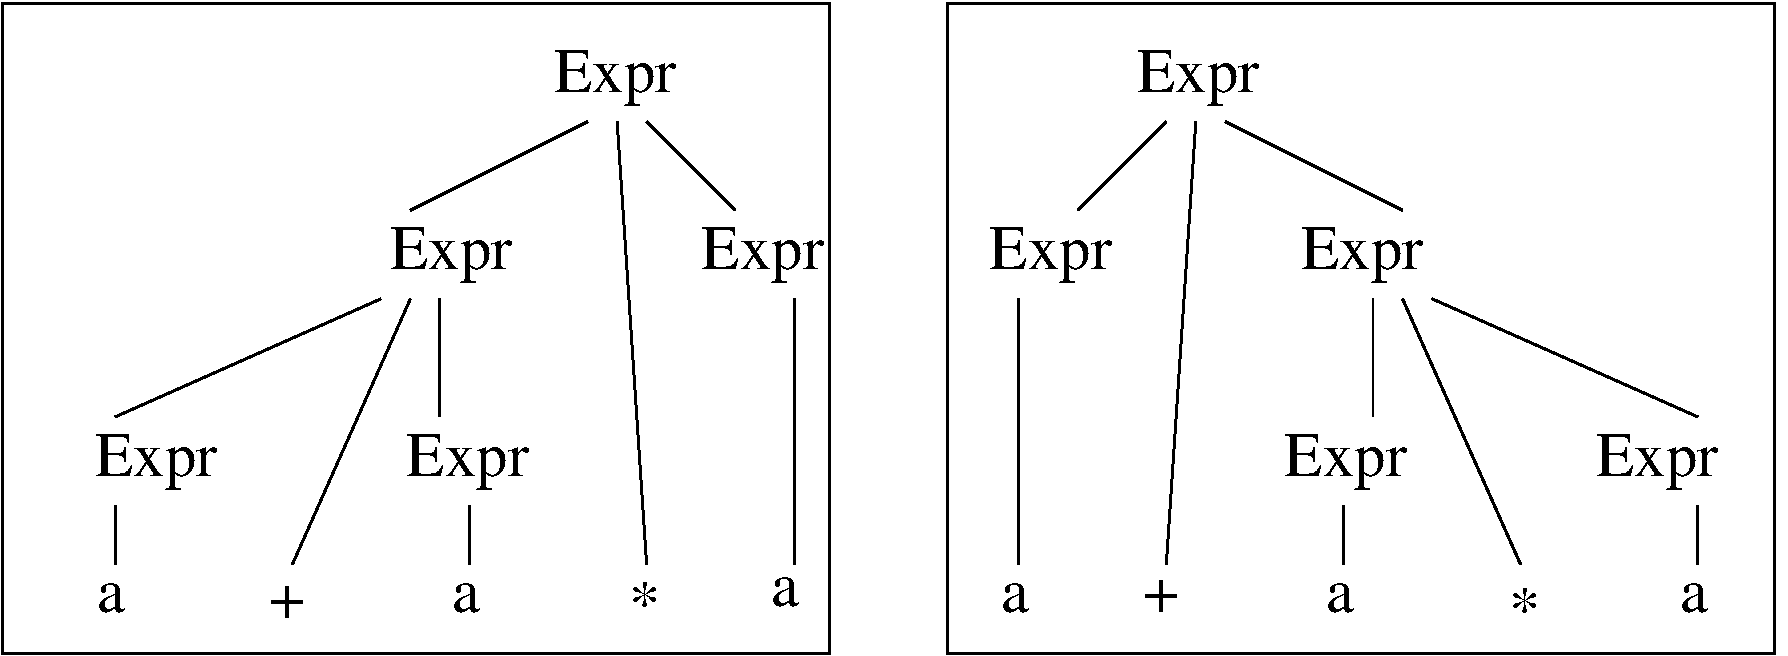
\includegraphics[%
  width=0.7\linewidth,
  keepaspectratio]{ambi1}\end{center}
\caption{Twee parse trees voor $a+a*a$\label{ambi1}}
\end{figure}

De string a+a*a heeft meerdere meest-linkse afleidingen en dus ook
meerdere parse trees: de string wordt daarom {\em ambigu} genoemd. We
noemen de grammatica Arit1 ambigu omdat er strings bestaan in
$L_{Arit1}$ die ambigu zijn t.o.v. Arit1. A priori is het niet duidelijk
of voor dezelfde taal ook een niet-ambigue grammatica bestaat. Eerst
een nuttige definitie:


\grijs{\begin{definitie} Equivalente CFG's \\
{\rm
Twee contextvrije grammatica's $CFG1$ en $CFG2$ zijn equivalent indien 

$~~~~~~~~~~~L_{CFG1} = L_{CFG2}$
}
\end{definitie}}

Je moet eigenlijk bewijzen dat dit een equivalentierelatie op de CFG's
definieert, maar dat is natuurlijk kinderspel voor jullie.




Hier is een andere CFG Arit2\label{arit2label}:

\begin{itemize}
\item Expr \rpijl Expr + Term
\item Expr \rpijl Term
\item Term \rpijl Term $*$ a
\item Term \rpijl a
\end{itemize}

Je kan nagaan dat Arit1 en Arit2 equivalent zijn.


Je kan ook nagaan dat $a+a*a$ nu enkel de meest-linkse afleiding 


$Expr \Rightarrow Expr + Term \Rightarrow Term + Term \Rightarrow a + Term$

$~~~~~~~~~~\Rightarrow a + Term * a \Rightarrow a + a * a$


heeft en dat elke string slechts \'{e}\'{e}n parse tree heeft voor Arit2.
Daarom noemen we Arit2 een niet-ambigue grammatica.


Niet elke contextvrije taal heeft een niet-ambigue CFG: zulk een
contextvrije taal heet {\em inherent ambigu}. Hier is een voorbeeld van
een inherent ambigue taal: $\{a^nb^nc^m,  a^nb^mc^m| n,m \geq 0\}$.
Het bewijs daarvan kan je vinden in het boek van
Hopcroft-Motwani-Ullman, maar bewijs zelf dat de taal contextvrij is!
Later hebben we het nog over ambigu\"{i}teit.


Als een niet-terminaal symbool aan de linkerkant van meerdere regels
voorkomt, dan kunnen we die samennemen. Bijvoorbeeld kan grammatica
Arit2 ook beschreven worden als:
\begin{itemize}
\item Expr \rpijl Expr + Term $|$ Term
\item Term \rpijl Term $*$ a $|$ a
\end{itemize}



\clearpage
\subsection{CFG's in een speciale vorm}

Soms is het handig een meer restrictieve vorm van een grammatica te
hebben, liefst zonder contextvrije talen uit te sluiten. Hier is zulk
een vorm:

\grijs{\begin{definitie} Chomsky Normaal Vorm\\
{\rm
Een CFG heeft de Chomsky Normaal Vorm als elke regel \'{e}\'{e}n van
de volgende vormen heeft:
\begin{enumerate}
\item A \rpijl BC
\item A \rpijl $\alpha$
\item S \rpijl $\epsilon$
\end{enumerate}

Daarin is $\alpha$ een eindsymbool, A is een niet-eindsymbool, en B en C
zijn niet-eindsymbolen verschillend van S (het startsymbool).  }
\end{definitie}}

Soms laat men de regel S \rpijl $\epsilon$ niet toe: dan kan die CFG
niet de lege string afleiden natuurlijk.



\grijs{
\begin{stelling}\label{chomskynormalform}
Voor elke contextvrije grammatica bestaat een equivalente contextvrije
grammatica in Chomsky Normaal Vorm.
\end{stelling}}
\begin{proof}
We geven een constructief bewijs: het is lang maar niet moeilijk. We
vertrekken van een willekeurige CFG en transformeren hem terwijl we
equivalentie bewaren naar Chomsky Normaal Vorm.

\begin{enumerate}
\item[{\bf 1.}] We beginnen met te zorgen dat er een startsymbool is
dat alleen links in een regel voorkomt: als S het startsymbool is in
de grammatica, vervang het dan overal door een nieuw niet-eindsymbool
(bijvoorbeeld X) en voeg de regel $S \rightarrow X$ toe 

\item[{\bf 2.}] Daarna voldoen we aan de derde eis van Chomsky Normaal Vorm:

stel dat we een regel ${\cal E} = A \rightarrow \epsilon$ hebben en
een regel ${\cal R} = B \rightarrow \gamma$ waarin A voorkomt in
$\gamma$, dan defini\"eren we de verzameling regels $V({\cal E},{\cal
R})$ als de verzameling regels van de vorm $B \rightarrow \eta$
waarbij $\eta$ verkregen wordt uit $\gamma$ door elke combinatie van
voorkomens van A in $\gamma$ weg te laten.  

We transformeren de grammatica dan als volgt:

\begin{itemize}
\item[]
zolang er regels ${\cal E} = A \rightarrow \epsilon$ en
een regel ${\cal R} = B \rightarrow \gamma$ waarin A voorkomt zijn
zodanig dat $V({\cal E},{\cal R})$ nieuwe regels bevat, voeg $V({\cal
E},{\cal R})$ toe aan de grammatica
\end{itemize}
Zorg dat je inziet dat dit eindigt!


Daarna (dus ook nadat je het ingezien hebt :-) verwijderen we uit de
bekomen grammatica alle regels van de vorm $A \rightarrow \epsilon$,
behalve als $A = S$: dit mag de enige regel zijn die \eps afleidt.


Zorg dat je inziet dat de bekomen grammatica nog dezelfde taal
bepaalt: je kan dat doen door te redeneren op afleidingen.


\item[{\bf 3.}] Nu willen we afgeraken van de regels van de vorm $A \rightarrow B$. 
Voor een regel van de vorm ${\cal E} = A \rightarrow B$ en een regel
van de vorm ${\cal R} = B \rightarrow \gamma$, definieer de regel
$U({\cal E},{\cal R}) = A \rightarrow \gamma$.

\begin{itemize}
\item[]
zolang er regels van de vorm ${\cal E} = A \rightarrow B$ (waarin B
ook een niet-terminal is) en ${\cal R} = B \rightarrow \gamma$ bestaan
en $U({\cal E},{\cal R})$ een nieuwe regel is, voeg $U({\cal E},{\cal
R})$ toe aan de grammatica
\end{itemize}
Zorg dat je inziet dat dit eindigt!


Daarna (dus ook nadat je het ingezien hebt :-) verwijderen we uit de
bekomen grammatica alle regels van de vorm $A \rightarrow B$.


Zorg dat je inziet dat de bekomen grammatica nog dezelfde taal
bepaalt: je kan dat doen door te redeneren op afleidingen.


\item[{\bf 4.}] We hebben nu nog 3 soorten regels te behandelen:
\begin{enumerate}
\item 
$A \rightarrow \gamma$ waar $\gamma$ uit juist twee niet-terminalen
bestaat: die laten we gerust

\item 
$A \rightarrow \gamma$ waar $\gamma$ minstens twee symbolen bevat:
vervang elke terminal $a$ door een nieuwe niet-terminaal $A_a$ en voeg
de regel $A_a \rightarrow a$ toe

\item 
eventueel $S \rightarrow \epsilon$: die mag blijven

\end{enumerate}
Zorg dat je inziet dat dit eindigt en dezelfde taal genereert!


\item[{\bf 5.}] de regels van de vorm $A \rightarrow X_1X_2...X_n$ met $n > 2$
    vervang je door \\ $A \rightarrow X_1Y_1$, $Y_1 \rightarrow X_2Y_2$, ...,
$Y_{n-2} \rightarrow X_{n-1}X_n$

% $A \rightarrow X_1Y_n$ en voeg nieuwe regels toe
%     van de vorm $Y_i \rightarrow Y_{i-1}X_i$ voor i=2..n
\end{enumerate}

Zorg dat je inziet dat dit eindigt en dezelfde taal genereert!


Is aan alle eisen voldaan nu?
\end{proof}


De Chomsky normaal vorm heeft als voordeel dat we direct kunnen zien
of de taal van een grammatica de lege string bevat, en dat elke parse
tree (bijna) een volledige binaire boom is: dat zal van pas komen in
het pompend lemma voor CFL's. Bovendien heeft elke afleiding van een
string van lengte $n > 0$ lengte $2n-1$. 



Er bestaan nog een andere normaalvormen voor CFG's: bijvoorbeeld de
Greibach\footnote{Sheila Greibach} normaal vorm laat enkel regels toe
van de vorm
\begin{itemize}
\item A \rpijl aX
\item S \rpijl \eps
\end{itemize}
waarin X een (mogelijk lege) sequentie is van niet-terminalen, en a
een terminal. Het voordeel van die vorm is dat een afleiding van een
string van lengte $n$ niet langer kan zijn dan $n$. Als
oefening kan je ook het analoog van de stelling op pagina
\pageref{chomskynormalform} bewijzen voor de Greibach normaal vorm.

\paragraph{Zelf doen:}
\begin{itemize}
\item[]
Bewijs dat een afleiding van een string van lengte $n > 0$ uit een
grammatica in Chomsky normaalvorm lengte $2n-1$ heeft.

Bewijs dat een afleiding van een string van lengte $n > 0$ uit een
grammatica in Greibach normaalvorm lengte $n$ heeft.

Kan je de transformatie naar Chomsky normaalvorm gebruiken om in te
zien dat elke (zuiver) Prologprogramma kan getransformeerd worden naar
een equivalent Prologprogramma met in elke clause juist nul of twee
doelen?
\end{itemize}


\clearpage
\section{De push-down automaat}

Een FSA heeft behalve zijn toestand geen geheugen. Doordat er maar een
eindig aantal toestanden zijn, kan een FSA dus niet onbegrensd {\em
tellen} en niet al te veel talen bepalen. Een push-down automaat heeft
een onbeperkt geheugen, doch het kan slechts op een beperkte manier
gebruikt worden: het geheugen is georganiseerd als een stapel (of
stack) en daarvan kan op elk ogenblik enkel de top ge\"{i}nspecteerd
worden. Verder kunnen er elementen worden bijgezet of afgehaald. Net
zoals bij de reguliere automaten gebruiken we een PDA om van een
string na te gaan of ie geaccepteerd wordt of niet: dat gebeurt door
opeenvolgende tekens van de string te consumeren en afhankelijk van de
huidige toestand en dat teken, naar een andere toestand over te
gaan. Bij de PDA komt daar nog bij dat die overgang kan afhangen van
de top van de stack, en dat er een teken kan bijgezet worden op de
stack. Net zoals bij de reguliere automaten defini\"eren we de PDA
direct met niet-determinisme.


\grijs{\begin{definitie} Een push-down automaat\\
{\rm Een push-down automaat is een 6-tal
$(Q,\Sigma,\Gamma,\delta,q_s,F)$ waarbij
\begin{itemize}
\item $Q$ is een eindige verzameling toestanden
\item $\Sigma$ is een eindig inputalfabet
\item $\Gamma$ is een eindig stapelalfabet
\item $\delta$ is een overgangsfunctie met signatuur
%
$Q \times \Sigma_\epsilon \times \Gamma_\epsilon \rightarrow {\cal P}(Q \times  \Gamma_\epsilon)$
\item $q_s$ is de starttoestand
\item $F \subseteq Q$ is een verzameling eindtoestanden

\end{itemize}

}
\end{definitie}}

Deze definitie zegt nog niks over de werking. Eerst een grafische
voorstelling van een PDA, in de stijl van de grafische voorstelling
van een FSA. Als voorbeeld nemen we de PDA
$(Q,\Sigma,\Gamma,\delta,q_s,F)$ met

\begin{itemize}
\item $Q = \{q_s, q_f, x, y\}$
\item $F = \{q_f\}$
\item $\Sigma = \{a,b,c\}$
\item $\Gamma = \{m, \$\}$
\end{itemize}

\newpage
De $\delta$ van de PDA kan je zien in de grafische voorstelling ervan
in Figuur~\ref{pda2}.

\medskip
\begin{figure}[h]
\begin{center}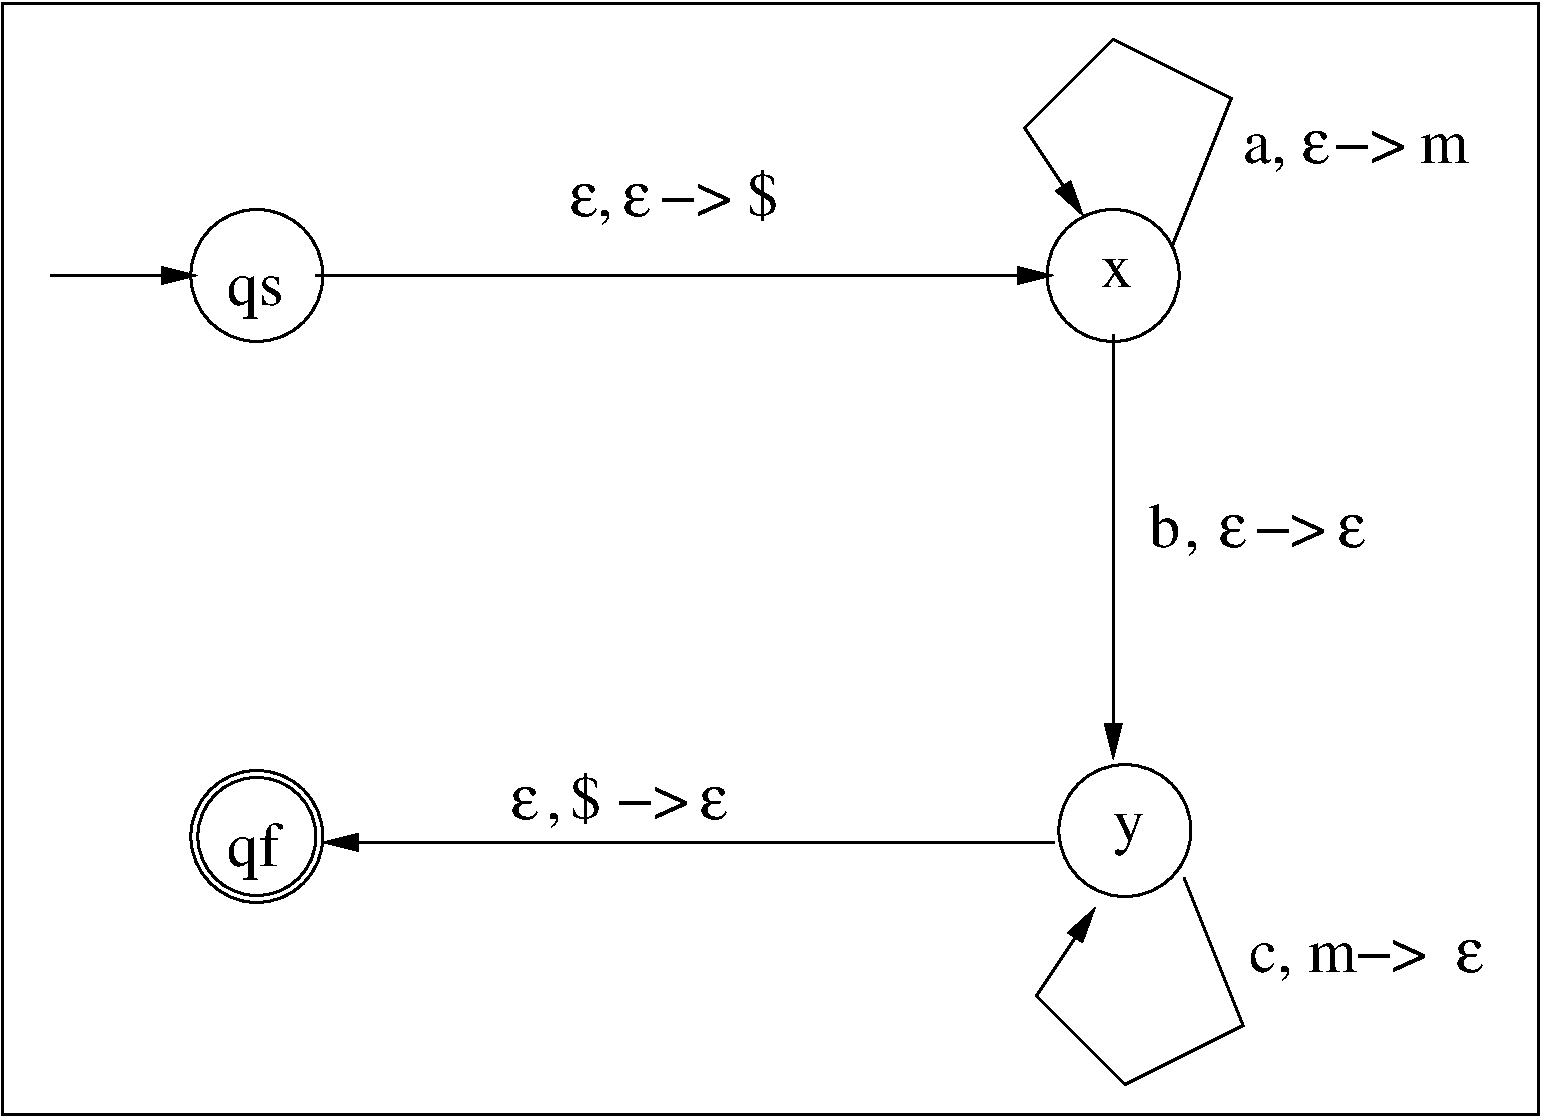
\includegraphics[%
  width=0.6\linewidth,
  keepaspectratio]{pda2}\end{center}
\caption{Een push-down automaat\label{pda2}}
\end{figure}

De bedoeling van een label zoals $\alpha,\beta \rightarrow \gamma$ op
een boog is

\begin{itemize}
\item indien $\alpha$ het eerste symbool is van de huidige string
\item en $\beta$ staat op de top van de stapel
\item volg dan de boog en
\begin{itemize}
\item verwijder $\alpha$ van de string
\item verwijder $\beta$ van de stapel
\item zet $\gamma$ op de stapel
\end{itemize}

\end{itemize}

Daarin mogen $\alpha$, $\beta$ en $\gamma$ ook $\epsilon$ zijn, wat voor
$\alpha$ wil zeggen: houd geen rekening met de huidige inputstring;
voor $\beta$: houd geen rekening met de huidige top van de stapel; voor
$\gamma$: push niets.

De bogen met hun labels specificeren dus de $\delta$.

Als we nu beginnen in $q_s$ met de string $a^2bc^2$, dan bevat de
stapel $mm\$$ op het ogenblik dat we de eerste keer in $y$ komen, en
de string bestaat nog uit $c^2$. Na nog twee keer $\delta$ toepassen
is de string helemaal geconsumeerd en nog \'{e}\'{e}n toepassing
brengt ons in de eindtoestand.  We zeggen: $a^2bc^2$ wordt
geaccepteerd door de PDA, of $a^2bc^2$ behoort tot de taal door de PDA
bepaald. Hier is een meer formele definitie van

\grijs{\begin{definitie} Aanvaarding van een string s door een PDA\\
{\rm
Een string s wordt aanvaard door een PDA indien s kan worden
opgesplitst in delen $w_i$, i= 1..m ($w_i \in \Sigma_\epsilon$), er
toestanden $q_j$, j= 0..m zijn, en stacks $stack_k$, k=0..m
($stack_k \in \Gamma^*$), zodanig dat
\begin{itemize}
\item $stack_0 = \epsilon$  (de stack is leeg in het begin)
\item $q_0 = q_s$ (we vertrekken in de begintoestand)
\item $q_m \in F$ (we komen aan in een eindtoestand met een lege string)
\item $(q_{i+1},y) \in \delta(q_i,w_{i+1},x)$ waarbij $x,y \in
\Gamma_\epsilon$ en

$stack_i = xt,~~stack_{i+1} = yt$ met $t \in \Gamma^*$
\end{itemize}


}
\end{definitie}}


De laatste bullet geeft aan dat de overgangen juist gebeuren volgens $\delta$.

\paragraph{Let op:}

Bovenstaande definitie zegt niets over de stackinhoud op het ogenblik
dat we in de eindtoestand komen: die zegt enkel dat we met een lege
string in een eindtoestand moeten geraken. Er bestaan alternatieve
definities van PDA: soms mag meer dan \'{e}\'{e}n symbool gepusht
worden in \'{e}\'{e}n overgang. Soms wordt acceptatie gedefinieerd
als: {\em de string is op en de stack is leeg} (dan is $F$ zelfs van geen
belang) en soms als {\em de string is op en de stack is leeg en we
zitten in een eindtoestand}. Uiteindelijk zijn al deze definities
equivalent wat betreft de talen die kunnen bepaald worden. Bijkomende
eisen kunnen zijn: in elke overgang wordt ofwel een symbool gepusht
ofwel gepopt maar niet beide, of er is slechts \'{e}\'{e}n
eindtoestand ...  maar ook dat verandert niets essentieels.

\project{ivm equivalentie van die dingen - misschien ook minimisatie
NFA/MN voor NFA}

\grijs{\begin{definitie} Taal bepaald door een PDA\\
{\rm
De taal L bepaald door een PDA bestaat uit alle strings die door de
PDA aanvaard worden.
}
\end{definitie}}


Het is duidelijk dat de taal $\{a^nbc^n|n \geq 0\}$ door een PDA
bepaald wordt: Figuur~\ref{pda2} gaf een implementatie. Strings zoals
aabc worden niet aanvaard.

% \newpage
Hoe tricky het is, zie je in Figuur~\ref{pda1}: op het eerste zicht
zou je kunnen denken dat die dezelfde taal aanvaardt, maar is dat wel
zo?

\begin{figure}[h]
\begin{center}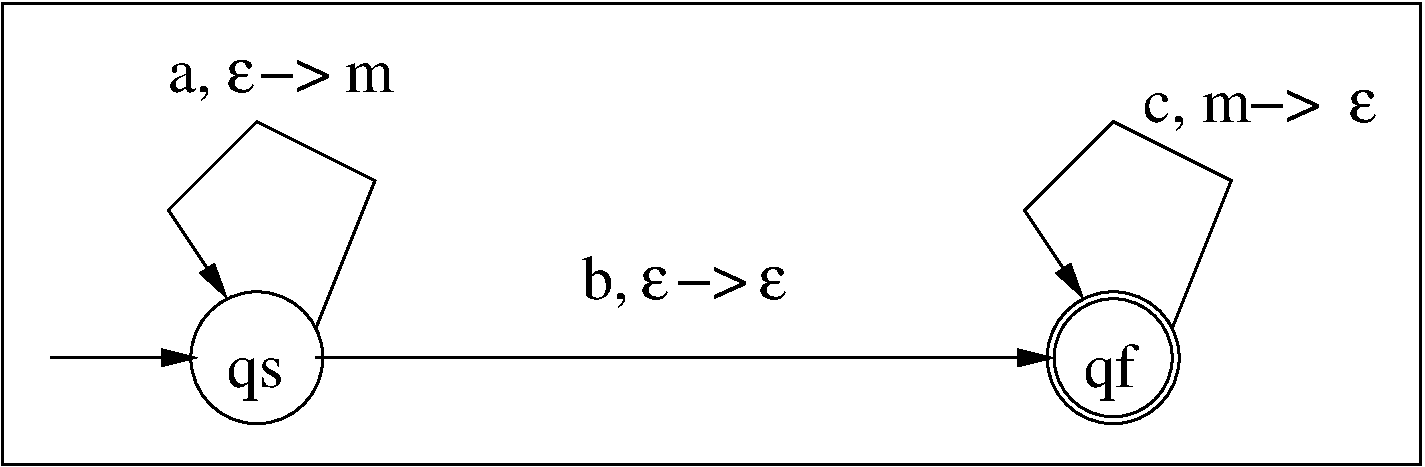
\includegraphics[%
  width=0.6\linewidth,
  keepaspectratio]{pda1}\end{center}
\caption{Een tweede push-down automaat\label{pda1}}
\end{figure}

Als je voor de PDA in Figuur~\ref{pda1} acceptatie definieert als {\em
aankomen in de eindtoestand met lege stack}, dan bepaalt deze PDA wel
dezelfde taal: de details van de definitie bepalen dus wel wat een
bepaalde PDA juist accepteert, maar niet de klasse van talen die door een
PDA kunnen bepaald worden.


% \clearpage
\section{Equivalentie van CFG en PDA}

We willen de volgende stelling bewijzen:

\grijs{\begin{stelling}
Elke push-down automaat bepaalt een contextvrije taal en elke
contextvrije taal wordt bepaald door een push-down automaat.
\end{stelling}}
\begin{proof}
Er zijn duidelijk twee delen in deze stelling. Het eerste deel
bewijzen we in het lemma op pagina \pageref{equicfgpda1}, het tweede
in het lemma op pagina \pageref{equicfgpda2}. \end{proof} 

Eerst wat voorbereidend werk en een voorbeeld.


We hebben voordien al eens gezegd dat in \'{e}\'{e}n push er meerdere
symbolen bij mogen komen op de stapel zonder dat dat de kracht van
PDA's verandert (als je het nog niet deed ... dit is een goed moment om
het te bewijzen). We gaan daarvan gebruik maken, omdat het de
beschrijving heel wat korter maakt.

% \clearpage
\begin{vb}
Beschouw de CFG Arit1 van pagina \pageref{arit1label}
\begin{itemize}
\item E \rpijl E + E~~~~~~~E \rpijl E * E~~~~~~~E \rpijl a
\end{itemize}
waarbij E het startsymbool is. En kijk nu eens naar de PDA in figuur
\ref{pda3}.

\begin{figure}[h]
\begin{center}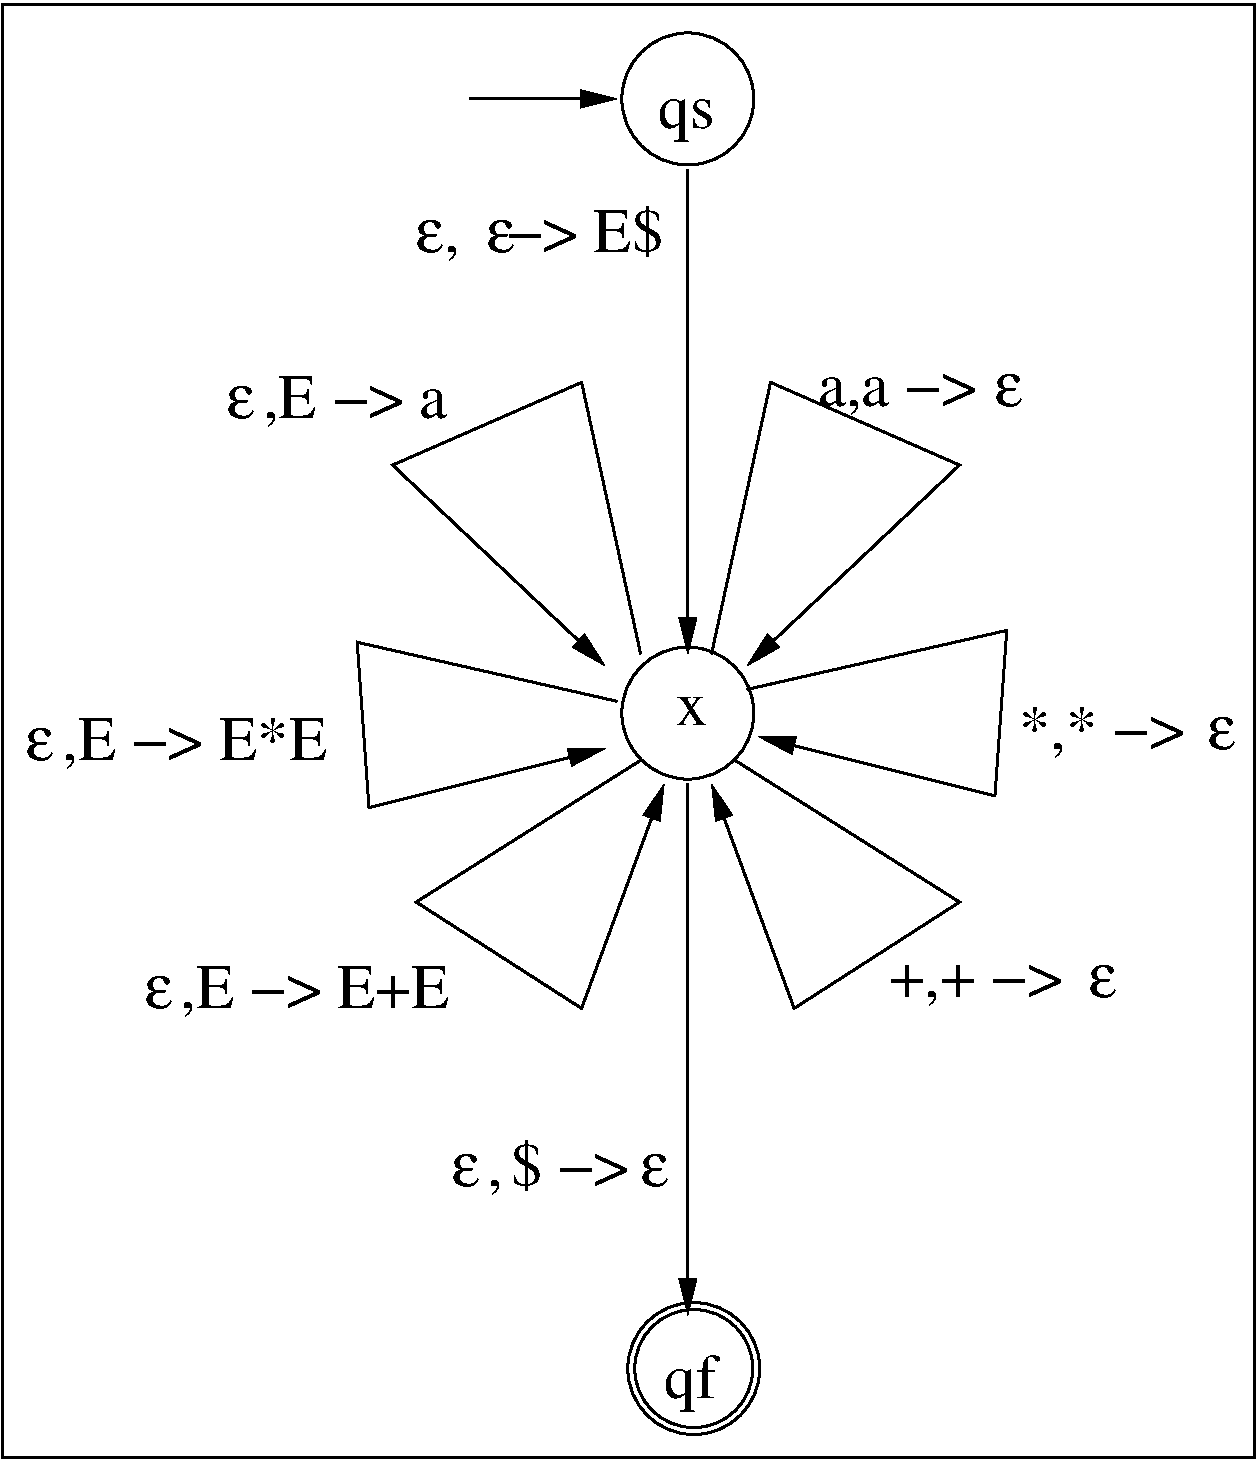
\includegraphics[%
  width=0.45\linewidth,
  keepaspectratio]{pda3}\end{center}
\caption{Een PDA afgeleid van Arit1\label{pda3}}
\end{figure}

Die PDA vertoont wat meer symmetrie dan je vertrekkend van een andere
grammatica zou krijgen, maar hij is op de volgende manier systematisch
geconstrueerd:
%
\begin{itemize}
\item er zijn slechts 3 toestanden: de begintoestand $q_s$, de eindtoestand $q_f$ en \'{e}\'{e}n hulptoestand $x$
\item er is slechts \'{e}\'{e}n boog van $q_s$ naar $x$: die kijkt
niet naar de string of de stapel, en zet een marker \$ op de stapel en
het beginsymbool
\item er is slechts \'{e}\'{e}n boog van $x$ naar $q_f$: die
consumeert niks van de string en haalt de marker \$ van de stapel
\item de andere bogen gaan van $x$ naar $x$; de labels corresponderen met
\begin{itemize}
\item de symbolen uit het invoeralfabet: voor elke $\alpha \in \Sigma$,
is er een boog met label $\alpha,\alpha \rightarrow \epsilon$; die bogen
betekenen dus: als de top van de stapel gelijk is aan het eerste
symbool van de string, consumeer dan beide
\item de regels van de grammatica: voor elke regel $X \rightarrow
\gamma$ is er een label $\epsilon, X \rightarrow \gamma$; die bogen
betekenen dus: als de top van de stapel een niet-eindsymbool X is,
vervang het door de rechterkant $\gamma$ van een regel in de grammatica
waarvan X de linkerkant is; $\gamma$ is een rij eind- en
niet-eindsymbolen
\end{itemize}

\end{itemize}
\end{vb}

\paragraph{Zelf doen:} Wat is de relatie tussen het inputalfabet en
het stapelalfabet enerzijds en de terminals en non-terminals van de
grammatica anderzijds?  

We gebruiken die PDA eens om de string $a+a*a$ te parsen: tabel
\ref{parsing1} laat de stapel en de string zien in de opeenvolgende
toestanden. Merk op dat als we een reeks symbolen XYZ op de stapel
willen pushen, we die eigenlijk in omgekeerde volgorde op de stapel
willen hebben, en de representatie van een stapel is dan ook een string
die we van voor aanvullen (zonder omkeren van XYZ) en waarvan we van
voor weer wegnemen.

% \clearpage
\begin{table}[ht]
\center
\begin{tabular}{|r|r|r|}
\hline
string     &  stapel      & toestand \\ \hline
a+a$*$a      & $\epsilon$   & $q_s$   \\
a+a$*$a      &   E\$        & $x$     \\
a+a$*$a      &   E$*$E\$       & $x$       \\
a+a$*$a      &   E+E$*$E\$     & $x$       \\
a+a$*$a      &   a+E$*$E\$     & $x$       \\
 +a$*$a      &    +E$*$E\$     & $x$       \\
  a$*$a      &   E$*$E\$       & $x$       \\
  a$*$a      &   a$*$E\$       & $x$       \\
   $*$a      &    $*$E\$       & $x$       \\
    a      &     a\$       & $x$       \\
$\epsilon$ &      \$       & $x$       \\
$\epsilon$ & $\epsilon$   & $q_f$    \\
\hline
\end{tabular}
\caption{Parsing van $a+a*a$} \label{parsing1}
\end{table}
Deze parsing geeft een meest-linkse afleiding. Die is niet
noodzakelijk uniek: als je bij de tweede overgang E+E kiest
i.p.v. E$*$E dan kom je er ook nog!  

Kan het zijn dat je vastloopt? Probeer eens om in de derde overgang
E*E te kiezen i.p.v. E$+$E en je ziet het. Is dat erg?


Ga nu na dat elke string die door de Arit1 wordt bepaald, door de PDA
in Figuur~\ref{pda3} wordt aanvaard en omgekeerd.


Dat voorbeeld generaliseren we direct tot het volgende lemma:

% \newpage
\grijs{\begin{lemma}\label{equicfgpda1}
De constructie van een PDA uit een CFG zoals hierboven gegeven, levert
een PDA die de taal $L_{CFG}$ accepteert.
\end{lemma}}
\begin{proof}
Je kan nagaan dat er een \'{e}\'{e}n-\'{e}\'{e}nduidig verband is
tussen een afleiding in de CFG van een string s en een accepterende
uitvoering van de PDA voor s.  \end{proof} 

Tenslotte nog een woordje over niet-determinisme en ambigu\"{i}teit: met
bovenstaande constructie van een PDA uit een CFG bekomen we een
niet-deterministische PDA indien er voor minstens \'{e}\'{e}n
niet-terminaal symbool twee regels bestaan. Dat lijkt ambigu\"{i}teit te
impliceren van de grammatica, maar dat is niet zo: ook grammatica
Arit2 op pagina \pageref{arit2label} geeft aanleiding tot een
niet-deterministische PDA (met bovengaande constructie) maar Arit2 is
een niet-ambigue grammatica.  

Langs de andere kant kan je je afvragen of de uitspraak {\em indien er
een deterministische PDA bestaat voor L, dan is L niet-ambigu} waar
is.


De constructie van een PDA uit een CFG is zo gemakkelijk: slechts drie
toestanden nodig en een heel uniforme beschrijving van de
overgangen. Het valt dan ook tegen dat we omgekeerd - van PDA naar CFG
- zo veel meer werk hebben ... immers, niet elke PDA heeft slechts drie
toestanden en onze methode van GNFA naar GNFA met slechts twee
toestanden lijkt hier niet te werken.  

% \newpage
Voor we de constructie beschrijven, veronderstellen we eerst dat de
PDA van een bepaalde vorm is:
\begin{itemize}
\item er is slechts \'{e}\'{e}n eindtoestand
\item de stapel wordt leeggemaakt voor we daarin terechtkomen
\item elke transitie neemt \'{e}\'{e}n symbool weg van de stapel, of
zet er \'{e}\'{e}n op, maar niet beide
\end{itemize}
We hebben die vorm al eens vermeld en je kan nu een bewijsje maken
dat dit niet restrictief is.

% \clearpage
\subsection{Constructie van een CFG $(V,\Sigma,R,S)$ uit een PDA
$(Q,\Sigma,\Gamma,\delta,q_s,\{q_f\})$:}
\begin{itemize}
\item $V = A_{p,q}$ waarbij $p, q \in Q$
\item $S = A_{q_s,q_f}$
\item $R$ bestaat uit drie delen:
\begin{itemize}
\item regels van de vorm $A_{p,p} \rightarrow \epsilon$ voor elke $p \in Q$
\item regels van de vorm $A_{p,q} \rightarrow A_{p,r}A_{r,q}$ voor
alle $p, q, r \in Q$
\item regels van de vorm $A_{p,q} \rightarrow aA_{r,s}b$ waarbij

$p, q, r, s \in Q, 
a,b \in \Sigma_\epsilon, 
t \in \Gamma,
(r,t) \in \delta(p,a,\epsilon),
(q,\epsilon) \in \delta(s,b,t)$
\end{itemize}

\end{itemize}


De intu\"{i}tie achter de constructie is de volgende: de strings die je
met een initieel lege stapel van toestand p naar q brengen met lege
stapel, worden gegenereerd door het niet-eindsymbool $A_{p,q}$.

\grijs{\begin{lemma}\label{equicfgpda2}
Bovenstaande constructie van een CFG uit een PDA bewaart de taal.
\end{lemma}}
\begin{proof}
Het bewijs wordt dit jaar niet gezien.
\end{proof}


\paragraph{Gevolg I:} als een taal door een PDA wordt bepaald, dan is
die taal contextvrij.

\paragraph{Gevolg II:} elke reguliere taal is contextvrij. Dat komt
doordat een FSA eigenlijk enkel maar een PDA is waarbij de stapel
nooit meespeelt in de beslissingen.

\paragraph{Zelf doen:} 
Er was een andere manier om in te zien dat elke reguliere taal
contextvrij is: stel voor een gegeven reguliere taal een CFG op.

\paragraph{Afsluiter:} We vermelden nog twee stellingen die inzicht
geven in de structuur van contextvrije talen. De
Chomsky-Sch\"{u}tzenberger stelling zegt dat elke contextvrije taal
essentieel de doorsnede is van een reguliere taal met een {\em geneste
haakjestaal}\footnote{Die geneste haakjestalen worden ook wel Dyck
talen genoemd, naar Walther von Dyck.} (mogelijk met meerdere soorten
haakjes). De stelling van Parikh kan geformuleerd worden met behulp
van een transformatie $Ord$ van een taal: voor een gegeven string $s$
is $Ord(s)$ de string die je verkrijgt door de symbolen van $s$ in
alfabetische volgorde te zetten. Bijvoorbeeld $Ord(bacabbc) =
aabbbcc$. Parikh zegt nu dat voor elke contextvrije taal L er een
reguliere taal R bestaat zodat $Ord(L) = Ord(R)$. M.a.w. afgezien van
de volgorde van de symbolen zijn regulier en contextvrij gelijk!

\project{Parikh of Chomsky-Sch\"{u}tzenberger uitwerken}

\clearpage
\section{Een pompend lemma voor Contextvrije Talen}\label{pompcfl}

\grijs{\begin{stelling}
Voor een contextvrije taal L bestaat een getal p (de pomplengte) zodanig dat
elke string s van L met lengte minstens p kan opgedeeld worden in 5
stukken u,v,x,y en z uit $\Sigma^*$ zodanig dat s = uvxyz
\begin{enumerate}
\item $\forall i \geq 0: uv^ixy^iz \in L$
\item $|vy| > 0$
\item $|vxy| \leq p$
\end{enumerate}
\end{stelling}}
\begin{proof}
We gebruiken weer het duivenhokprincipe, maar nu op de parsetree voor
lang genoege strings. Neem eerst een CFG in Chomsky normaalvorm voor
L: dat werkt iets gemakkelijker, want elke regel heeft nu ofwel twee
ofwel nul niet-terminalen aan de rechterkant. Laat het aantal
niet-eindsymbolen in de CFG $n$ zijn.
\end{proof}


Voor een string s uit L bestaat er een parse tree.
Als je van die boom de onderste takken wegsnoeit hou je een volledige
binaire boom over want de grammatica staat in Chomsky normaalvorm. Die
boom heeft hoogte minstens gelijk aan $log_2(|s|)$. Het langste
enkelvoudig pad van de wortel van die boom bevat dus minstens
$log_2(|s|) + 1$ knopen en als we $s$ lang genoeg kiezen, dan is
$log_2(|s|) + 1$ groter dan $n$ en bijgevolg moet er op dat langste
pad minstens \'{e}\'{e}n niet-eindsymbool - zeg X - herhaald
worden. Neem de laagste X (noteren we door $X_2$) en zijn dichtste
herhaling ($X_1$) op dat pad - X is zeker verschillend van het
startsymbool (waarom?). Zie Figuur~\ref{parsetree2} voor een
voorstelling van de zaken. We kunnen nu uit die parse tree een
afleiding construeren waarvan we enkel wat tussenstappen laten zien:


$~~~~~~~~S \Rightarrow^* uX_2z \Rightarrow^* uvX_1yz \Rightarrow^* uvxyz$ (a)


In die afleiding zijn u,v,x,y,z strings uit $\Sigma^*$ en bovendien
zijn v en y niet tegelijkertijd leeg, want dan zou men uit X zichzelf
kunnen afleiden en dat kan niet wegens de vorm van de grammatica.

Vermits (a) een geldige afleiding is, is


$~~~~~~~~S \Rightarrow^* uX_2z \Rightarrow^* uxz$


dat ook en ook


$~~~~~~~~S \Rightarrow^* uXz \Rightarrow^* uvXyz \Rightarrow^* uvvxyyz$


is er eentje en ...


We hebben dus al (1) en (2) van de opgave van de stelling, als we
strings nemen die langer zijn dan $2^{(n-1)}$: dat wordt onze pomplengte
p.


We besluiten nu ook (3): vxy wordt afgeleid vanuit X met een parse
tree die kleiner is dan $n$, dus hoogstens $2^{n-1}$ bladeren heeft en die
corresponderen juist met vxy. Figuur~\ref{parsetree2} verduidelijkt
dat nog eens.
\prend
\begin{figure}[h]
\begin{center}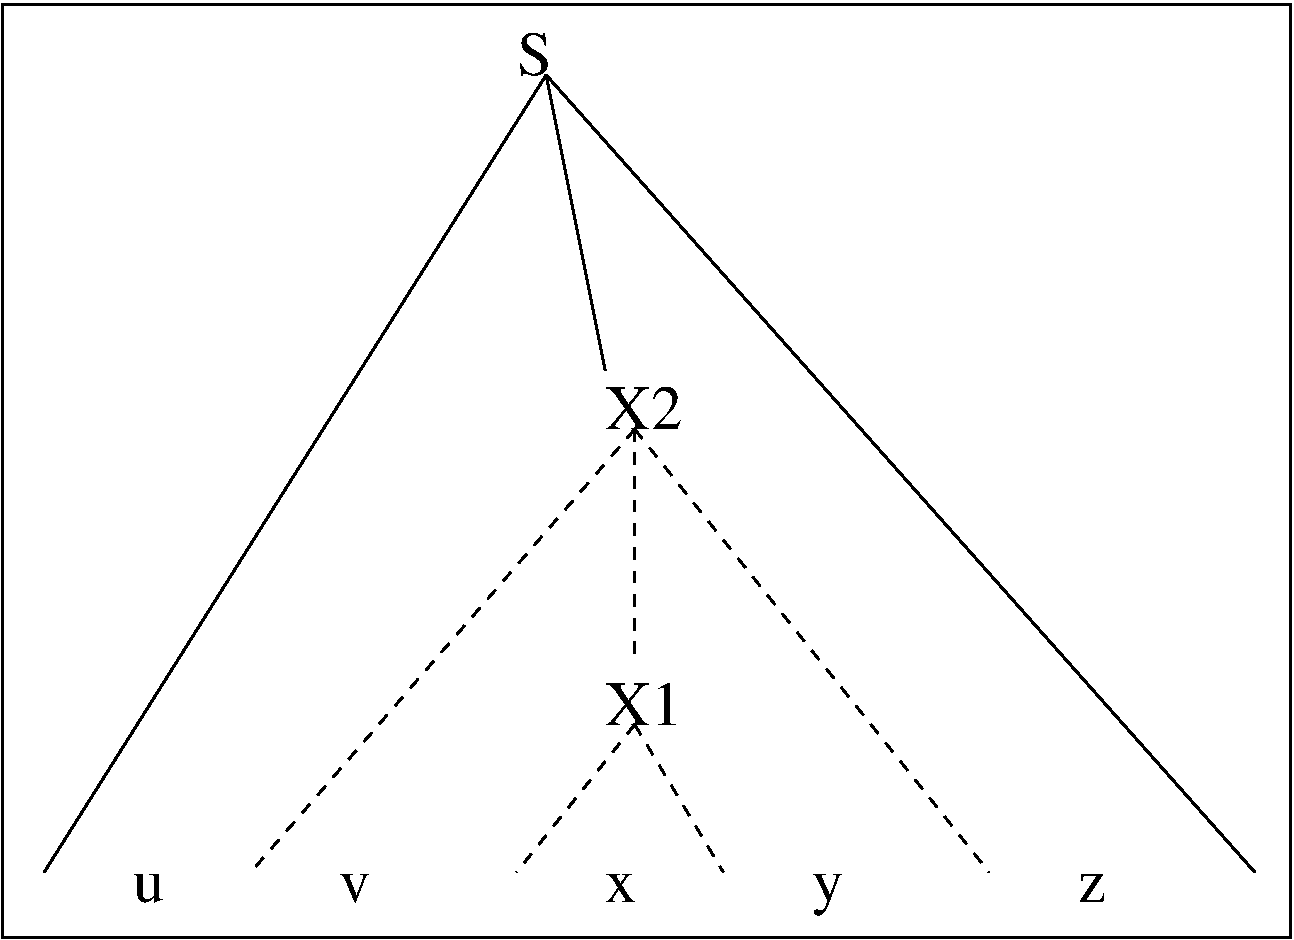
\includegraphics[%
  width=0.35\linewidth,
  keepaspectratio]{parsetree2}\end{center}
\caption{De parse tree met de repeterende non-terminal X \label{parsetree2}}
\end{figure}


\subsection{Toepassing van het pompend lemma voor CFL's}\label{voorbeeldpompcfl}

Neem de taal $L = \{a^nb^nc^n | n \geq 0\}$. Stel dat er een pomplengte p
bestaat. Neem een string s die langer is, namelijk $s = a^pb^pc^p$.
Stel dat $s = uvxyz$ met $|vy| > 0$. Dan zijn er twee mogelijkheden:
\begin{enumerate}
\item
v is van de vorm $\alpha^k$ en y is van de vorm $\beta^l$ waarbij
$\alpha$ en $\beta$ in $\{a,b,c\}$ zitten; daarbij is $k+l > 0$; in
dat geval kan $uv^2xy^2z$ niet bestaan uit een gelijk aantal a's, b's
en c's

\item
v of y bevat meer dan \'{e}\'{e}n symbool uit $\{a,b,c\}$; in dat
geval bevat $v^2$ of $y^2$ die symbolen niet in de juist volgorde en
zit $uv^2xy^2z$ niet in de taal

\end{enumerate}

Gevolg: $s$ kan niet gepompt worden en dus is L niet contextvrij.


\clearpage
\section{Een algebra van contextvrije talen?}

Voor de unie van twee contextvrije talen bepaald door de grammatica's
$CFG_1$ en $CFG_2$\footnote{Hernoem eerst de niet-eindsymbolen zodat ze
disjunct zijn.} kunnen we gemakkelijk een CFG maken: stel dat de
startsymbolen $S_1$ en $S_2$ zijn, maak dan een grammatica met de unie
van de regels van de $CFG_i$, voeg de regels $S_{new} \rightarrow S_i$
toe en neem $S_{new}$ als nieuwe startsymbool. Daarmee is bewezen dat
de verzameling van contextvrije talen gesloten is voor de unie operator.


Hoe zit het met de doorsnede van CFL's? Neem als eindsymbolen
$\{a,b,c\}$ en definieer $L_1 = \{a^nb^nc^m|n,m \geq 0\}$ en
$L_2 = \{a^nb^mc^m|n,m \geq 0\}$. Het is duidelijk dat de $L_i$
contextvrij zijn\footnote{Stel een CFG op voor die talen.}. De
doorsnede van de $L_i$ is echter de taal $\{a^nb^nc^n|n \geq 0\}$ en
daarvan hebben we in Sectie~\ref{voorbeeldpompcfl} bewezen dat die taal niet
contextvrij is. Dus: de doorsnede van contextvrije talen is niet
noodzakelijk contextvrij.  

We kunnen nu ook direct besluiten dat het complement van een CFL niet
contextvrij hoeft te zijn, want
%
$A \cap B$ = $\overline{(\overline{A} \cup \overline{B})}$.


Voor L contextvrij en A regulier kunnen we tenslotte ook nog kijken
naar de vragen:

\begin{itemize}
\item is $L \cup A$ contextvrij/regulier?
\item is $L \cap A$ contextvrij/regulier?
\end{itemize}

Wat denk je ervan?

\paragraph{Zelf doen:} Neem
%
$\Sigma = \{a,b\}$. De taal $\{ss|s \in \Sigma^*\}$ is niet
contextvrij. Bewijs dat. Laat zien dat het
\label{zelfdoen1} complement van die taal wordt gegenereerd door de
contextvrije grammatica:
\begin{itemize}
\item S \rpijl AB $|$ BA $|$ A $|$ B
\item A \rpijl CAC $|$ a
\item B \rpijl CBC $|$ b
\item C \rpijl a $|$ b
\end{itemize}

\clearpage
\section{Ambigu\"{i}teit en determinisme}

We kijken hier wat meer in detail naar het verband tussen de inherente
ambigu\"{i}teit van een contextvrije taal en zijn determinisme. We noteren
door DCFL de verzameling van contextvrije talen die een
deterministische PDA hebben (DPDA).


Een ambigue taal kan onmogelijk deterministisch zijn, dus
deterministische talen zijn niet-ambigu.  

\project{dit verder uitspitten}

Omgekeerd is niet waar: er bestaan niet-ambigue talen die niet
deterministisch zijn. Een standaard voorbeeld is 
de taal $\{ s\hat{s} | s \in \{a,b\}^*\}$ waarin $\hat{s}$ de omgekeerde
string betekent. Een niet-ambigue grammatica voor deze taal is
\begin{itemize}
\item[] S \rpijl aSa $|$ bSb $|$ \eps
\end{itemize}
maar een PDA weet van tevoren niet waar het midden van de string is en
moet daarnaar {\em raden}: dat is de essentie van het
niet-determinisme nodig om die taal te parsen. Dat betekent natuurlijk
niet dat er geen deterministische parser mogelijk is voor deze taal:
je kan er gemakkelijk eentje schrijven in Java. Maar het kan niet met
een deterministische PDA.


Een andere manier om een niet-deterministische taal te vinden is te
steunen op de eigenschap dat het complement van een DCFL ook DCFL is
\footnote{Voor een bewijs zie bijvoorbeeld het boek van Kozen.}. Neem
nu de taal $L = \{ss| s \in \{a,b\}^*\}$. Je kan met het pompend lemma
bewijzen dat L niet CFL is. $\overline{L}$ is echter contextvrij:
pagina \pageref{zelfdoen1} bevat er een CFG voor. Bijgevolg is
$\overline{L}$ geen DCFL.  

Voorbeelden van niet-deterministische talen worden dikwijls verkregen
door de unie te nemen van twee CFL's die overlappen: de taal


$~~~~~~~~~~~~~L = \{a^mb^nc^k| m \neq n\} \cup \{a^mb^nc^k|n \neq k\}$ is de unie van
twee DCFL's.


Stel dat L een DCFL was, dan zou zijn complement dat ook
zijn, en dan ook de intersectie van dat complement met de reguliere
taal $\{a^*b^*c^*\}$, maar dat geeft de taal $\{a^nb^nc^n|n \in \N\}$
en die taal is niet eens contextvrij!  

Hier is nog een niet-deterministische taal en een schets van een
constructie die dat bewijst:
$L = \{a^nb^n|n \in \N\} \cup \{a^nb^{2n}|n \in \N\}$.

\newpage
Stel dat er een DPDA M bestaat voor $L$, dan heeft die de structuur
zoals in Figuur~\ref{dpda1}.

\medskip
\begin{figure}[h]
\begin{center}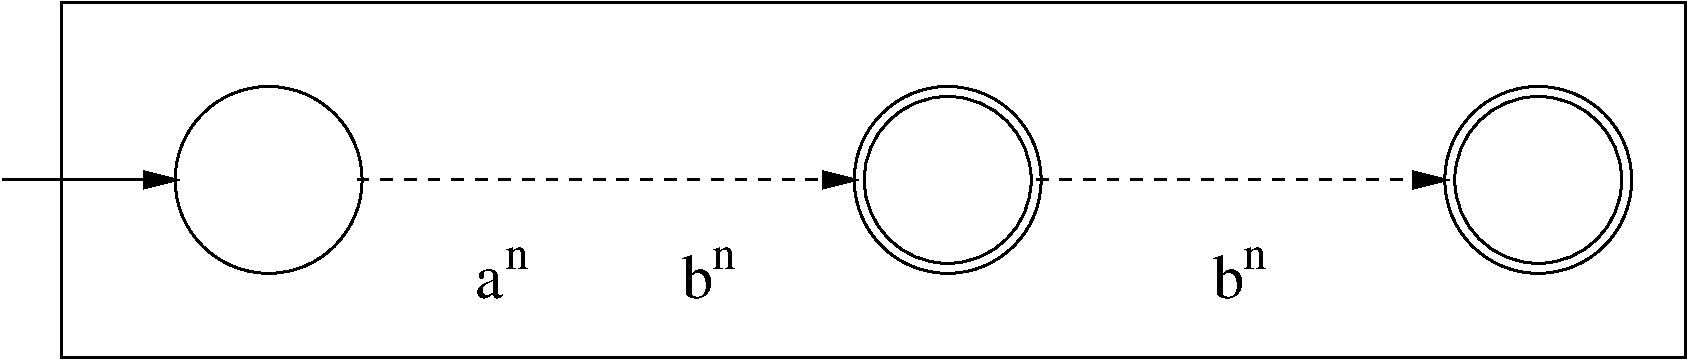
\includegraphics[%
  width=0.6\linewidth,
  keepaspectratio]{dpda1}\end{center}
\caption{De DPDA voor L\label{dpda1}}
\end{figure}

Vervang in het laatste deel de b's door c, en maak van de linkse
accepterende toestand een gewone toestand. Dan krijg je de machine in
Figuur~\ref{dpda2}.


\begin{figure}[h]
\begin{center}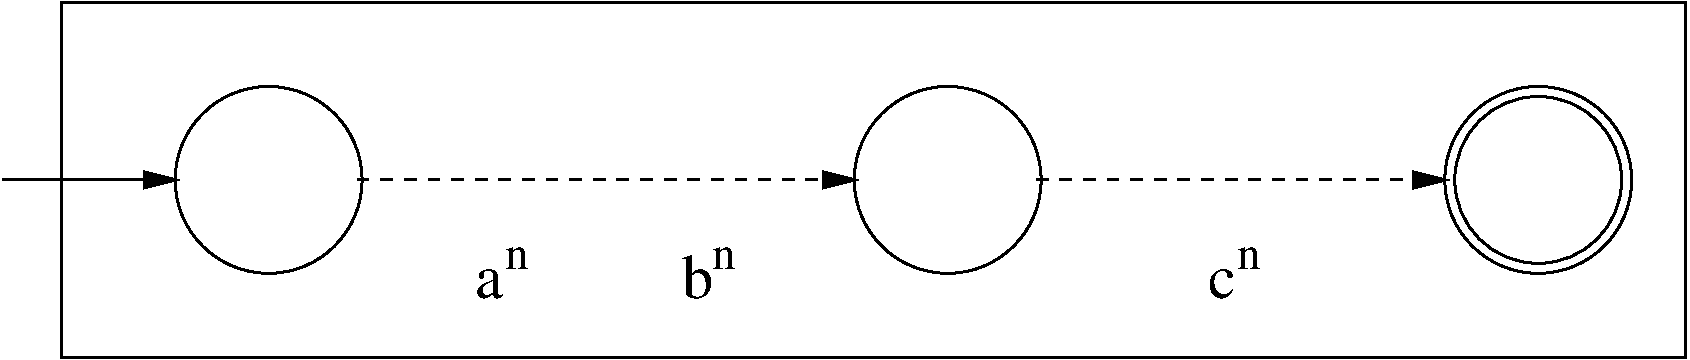
\includegraphics[%
  width=0.6\linewidth,
  keepaspectratio]{dpda2}\end{center}
\caption{De DPDA voor L'\label{dpda2}}
\end{figure}

Deze PDA accepteert de taal $L' = \{a^nb^nc^n|n \in \N\}$ maar we weten al
dat die laatste taal niet contextvrij is!  

Het boek van Linz bevat een variante met meer details.



Het belang van bovenstaande redenering/voorbeeld is dat wat waar was
voor reguliere talen (elke reguliere taal wordt bepaald door een
deterministische FSA) niet waar is voor CFL's en PDA's: door
\'{e}\'{e}n stapje hoger in de Chomsky hi\"erarchie te gaan, speelt
niet-determinisme ineens een belangrijke rol.

\clearpage
\section{Praktische parsingtechieken}

Dikwijls worden we geconfronteerd met het probleem: gegeven de
specificatie van een taal, maak er een herkenner voor.  Die taal kan
bijvoorbeeld zijn wat in een vakje op een formulier kan worden
ingevuld: dat kan afhangen van wat er elders al is ingevuld
(bijvoorbeeld mag je niet 3 namen van kinderen invullen, als je elders
declareerde dat je er maar 2 hebt). Die taal kan een programmeertaal
zijn met een ingewikkelde structuur: geneste if-then-else, statement
blocks, aritmetische expressies, package qualificaties ... Meestal is
zulk een taal contextvrij en het is de gewoonte om de beschrijving van
een programmeertaal in twee niveaus te doen: het eerste niveau is
lexicaal (zie pagina \pageref{flexlabel}) en het andere
syntactisch. Men maakt dan gebruik van de BNF-notatie. BNF staat voor
Backus\footnote{Turing award in 1977}-Naur\footnote{Turing award in
2005} form en werd voor de eerste keer gebruikt om Algol\footnote{Zoek
Algol op: het is een belangrijke stap in language design geweest!} te
beschrijven\footnote{Er is een hele historie aan verbonden, o.a. of
Naur er wel bij moet, en of anderen niet het krediet moeten krijgen
... kijk eens in wikipedia}. BNF trekt hard op CFG en we hebben het al
min of meer gebruikt op pagina \pageref{statlabel} voor de grammatica
van Stat.  

Net zoals flex vanuit een reguliere expressie omzet naar een
effici\"ente lexer, bestaan er tools die een CFG omzetten in een
effici\"ente syntax analyser. De algemene constructie van een PDA uit
een CFG is niet goed genoeg o.a. omdat het bijna altijd een
niet-deterministische automaat oplevert. Het deterministisch maken van
een PDA is niet eenvoudig (en zelfs niet altijd mogelijk zoals we
ondertussen weten). Daarom worden dikwijls extra beperkingen opgelegd
aan de talen/grammatica's die zulke parsergeneratoren aankunnen.  

Bekende parsergeneratoren zijn Bison (de opvolger van Yacc die C
genereert) en ANTLER (Java). Het praktische gebruik van deze tools
ligt buiten het bestek van deze cursus.


De automatisch geconstrueerde PDA uit een CFG gaf ons een meest-linkse
top-down afleiding: we vertrekken van het startsymbool en de boom wordt 
vanuit de wortel opgebouwd. Dat kan verwezelijkt worden in een
(deterministisch) programma door een {\em recursive descent parser}
m.b.v. een aantal wederzijds recursieve procedures die overeenstemmen
met de non-terminals in de grammatica. Dat werkt enkel als de
grammatica CFG van het type {\em LL(k)} is. Daarin staat de eerste $L$
voor: de input van Links naar rechts lezen; de tweede $L$ staat voor
Leftmost derivation; de $k$ staat voor het aantal tekens van de invoer
waarop de volgende beslissing genomen wordt, of wat men de {\em
look-ahead} noemt.  


Er is ook een andere manier: we gaan over de invoerstring van links
naar rechts en telkens als we iets zagen dat een rechterkant van een
regel is, dan gebruiken we die regel {\em omgekeerd}. Hier weer het
voorbeeld $a+a*a$ in een tabel zodat je kan zien wat al bekeken was en
wat niet.


\begin{table}[ht]
\center
\begin{tabular}{|l|r|l|}
\hline
al gezien  & nog te bekijken & te nemen actie \\ \hline
           & a+a$*$a           & shift    \\ 
   a       &  +a$*$a           & reduce   \\ 
   E       &  +a$*$a           & shift    \\ 
   E+      &  a$*$a            & shift    \\ 
   E+a     &   $*$a            & reduce   \\ 
   E+E     &  $*$a             & reduce   \\ 
   E       &  $*$a             & shift    \\ 
   E$*$      &   a             & shift    \\ 
   E$*$a     &                 & reduce   \\ 
   E$*$E     &                 & reduce   \\ 
   E       &                 & stop   \\ 
\hline
\end{tabular}
\caption{Bottom-up parsing van $a+a*a$} \label{bottomup}
\end{table}
De acties komen overeen met wat een shift-reduce parser doet: ofwel
het eerste teken van de input op de stack zetten (en de input pointer
shiften), ofwel wat op de stack staat reduceren m.b.v. een omgekeerde
grammaticaregel. De basis waarop de beslissing genomen wordt is hier
niet aangeduid, maar is voor shift-reduce parsers de huidige toestand
(die hier helemaal niet vermeld is) en de k eerste input
symbolen. Zulk een parser heet dan LR(k), waarbij de R aanduidt dat we
een meest-rechtse afleiding maken.


Het construeren van praktische parsers is een uitgebreid
onderzoeksdomein waarvan de verworvenheden nu gebruikt worden o.a. bij
de constructie van compilers, analyse van XML documenten ... Ook het
automatisch herstellen van fouten, genereren van syntax-directed
editors en relevante foutenmeldingen gebeurt op basis van
grammatica's.



% \begin{verbatim}

% Maak een CFG voor een RE

% Probeer eens een parsetree te maken voor RE's

% Greibach - Kuroda - Panini ...

% BNF voor programmeertalen

% \end{verbatim}

\clearpage
\section{Contextsensitieve Grammatica}

In de stap van regulier naar contextvrij hebben we recursie over de
non-terminals toegelaten, maar de linkerkant van een regel moest
altijd bestaan uit juist \'{e}\'{e}n nonterminal.


De volgende laag in de Chomsky-hi\"erarchie wordt gevormd door de
contextsensitieve talen, gegenereerd door contextsensitieve
grammatica's: de linkerkant van een regel mag nu een bijna
willekeurige string zijn van terminals en nonterminals, waarvan er
eentje herschreven wordt. Bijvoorbeeld: 

$~~~~~~~~~a\underline{X}Yz$ \rpijl $a\underline{bCD}Yz$ 


is een contextsensitieve grammaticaregel: enkel in de context van a
(langs links) en Yz (langs rechts) mag X herschreven worden tot bCD.
Er zijn alternatieve (equivalente) definities van wat juist een
contextsensitieve grammaticaregel is, maar we gaan er hier niet
dieper op in.


Een equivalente definitie van een contextsensitieve grammatica is dat
in een regel van de vorm $\alpha$ \rpijl $\beta$, altijd $|\alpha| \leq
|\beta|$.


Het is a priori natuurlijk niet duidelijk dat niet alle
contextsensitieve talen ook contextvrij zijn. Maar neem de taal
$\{a^nb^nc^n|n \in \N\}$ waarvan we vroeger aantoonden dat die niet
contextvrij is. Hier is een contextsensitieve grammatica (volgens de
equivalente definitie) voor die taal:

\begin{itemize}
\item[] S \rpijl abc
\item[] S \rpijl aSBc
\item[] cB \rpijl  Bc
\item[] bB \rpijl  bb 
\end{itemize}

\paragraph{Zelf doen}: bewijs dat de bovenstaande grammatica inderdaad
de gevraagde taal bepaalt.

\clearpage

Er bestaat ook een normaal vorm voor contextsensitieve grammatica's
(die de lege string niet genereren), nl. de Kuroda normaal vorm: elke
regel is van de vorm

\begin{itemize}
\item[] AB \rpijl CD
\item[] A \rpijl BC
\item[] A \rpijl B
\item[] A \rpijl a
\end{itemize}

met A,B,C en D nonterminals, en a een terminal.


Een contextsensitieve taal kan geparsed worden door een
niet-deterministische lineair begrensde automaat (LBA) - een klasse
automaten die strikt sterker is dan de push down automaten, en die we
in een volgend hoofdstuk zullen invoeren.  Pas als we wat
eigenschappen ervan kennen, zullen we zijn plaats in de hi\"erarchie
appreci\"eren.  LBA's zijn belangrijk omdat ze beslissingsproblemen
oplossen in $O(n)$-space!


\begin{wrapfigure}[7]{r}{.2\textwidth}
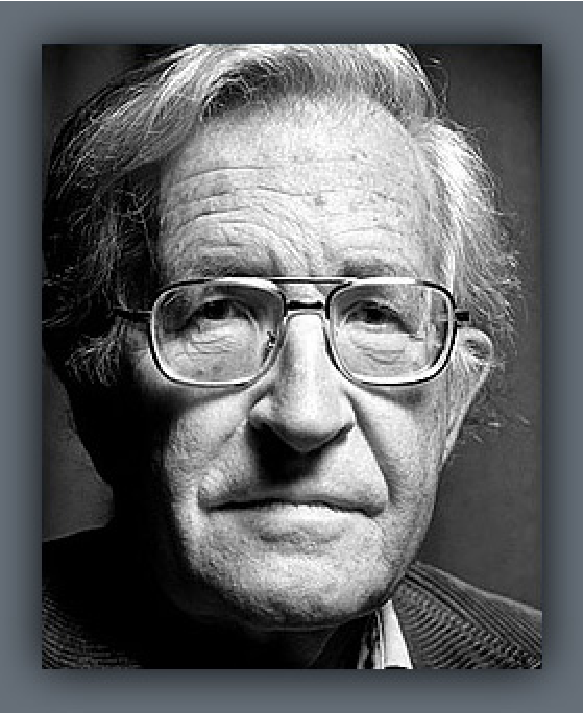
\includegraphics[width=.2\textwidth,keepaspectratio]{afbeeldingen/chomsky}
\end{wrapfigure}
Daarmee zijn we bijna aan de top van de Chomsky hi\"erarchie: 
als we de
laatste restrictie op de linkerkant van een regel wegnemen, dan komen
we bij de {\em unrestricted grammars}. De machinerie nodig om de
bijbehorende talen te parsen komt van de Turing machines: ook die
worden in een volgend hoofdstuk ingevoerd.


De hi\"erarchie zelf vind je in Tabel~\ref{chomskyhier}: er zijn
verfijningen (o.a. i.v.m. determinisme) maar die hebben we niet vermeld.

~\\
~\\
\begin{table}[ht]
\center
\begin{tabular}{|l|l|l|l|}
\hline
         & Grammatica          & Taal              & Automaat \\ \hline
Type-0   & unrestricted        & herkenbaar        & Turingmachine \\
Type-1   & context-sensitief   & context-sensitief & lineair-begrensd  \\
Type-2   & context-vrij        & context-vrij      & push-down \\
Type-3   & regulier            & regulier          & eindig  \\
\hline
\end{tabular}
\caption{De Chomsky-hi\"erarchie} \label{chomskyhier}
\end{table}


Chomsky is ook bekend om zijn politiek activisme - de moeite om eens
te lezen.


% \clearpage
% \section{Een toemaatje: Stochastische Contextvrije Grammatica}

% In een stochastische CFG (ook probabilistische CFG genoemd) wordt aan
% elke grammaticaregel een waarschijnlijkheid gegeven. Bijvoorbeeld:

% \begin{itemize}
% \item 0.7 Expr \rpijl Expr + Expr
% \item 0.3 Expr \rpijl Expr * Expr
% \item 1.0 Expr \rpijl a
% \end{itemize}

% Die kunnen we gebruiken om de waarschijnlijkheid van een afleiding
% te bepalen als het product van de waarschijnlijkheden van de gebruikte
% regels. Men kan dan zoeken naar de meest waarschijnlijke afleiding: in
% het geval van ambigue grammatica's voor natuurlijke talen geeft dat
% inzichten in wat meest waarschijnlijk bedoeld is (bijvoorbeeld als je
% aan speech recognition doet).
% 

